%        File: arfc-beamer.tex
%     Created: Sun May 5 10:00 PM 2013 C
%


%\documentclass[11pt,handout]{beamer}
\documentclass[9pt]{beamer}
\usetheme[white]{Illinois}
%\title[short title]{long title}
\title[Short Title]{Improved Delayed Neutron Group Parameters for Molten Salt Reactors}
%\subtitle[short subtitle]{long subtitle}
%\subtitle[Short SubTitle]{Improved MSR DNP Groups}
%\author[short name]{long name}
\author[Your Name]{Luke Seifert\\Advanced Reactors and Fuel Cycles Group}
%\date[short date]{long date}
\date[12.15.2025]{December 15, 2025}
%\institution[short name]{long name}
\institute[UIUC]{University of Illinois at Urbana-Champaign}

%\usepackage{bbding}
\usepackage{amsfonts}
\usepackage{amsmath}
\usepackage{xspace}
\usepackage{graphicx}
\usepackage{subfigure}
\usepackage{booktabs} % nice rules for tables
\usepackage{microtype} % if using PDF
\usepackage{bigints}
\usepackage{progressbar}
\usepackage{mathtools}
\usepackage{appendixnumberbeamer}
%\usepackage{minted}

\newcommand{\units}[1] {\:\text{#1}}%
\newcommand{\SN}{S$_N$}%{S$_\text{N}$}%{$S_N$}%
\DeclareMathOperator{\erf}{erf}
%I need some complimentary error functions...
\DeclareMathOperator{\erfc}{erfc}
%Those icons in the references are terrible looking
\setbeamertemplate{bibliography item}[text]

%%%% Acronym support

\usepackage[acronym,toc]{glossaries}
\newacronym{MOSART}{MOSART}{the Molten Salt Actinide Recycler and Transmuter reactor}
\newacronym{PIE}{PIE}{postulated initiating event}
\newacronym{DBA}{DBA}{design basis accident}
\newacronym{MPK}{MPK}{modified point kinetics}
\newacronym{CFD}{CFD}{computational fluid dynamics}
\newacronym{DPK}{DPK}{delayed point reactor kinetics}
\newacronym{MSR}{MSR}{fluid-fueled molten salt reactor}
\newacronym{TFM}{TFM}{Transient Fission Matrix}
\newacronym{MSRs}{MSRs}{fluid-fueled molten salt reactors}
\newacronym{RELAP}{RELAP}{the Reactor Excursion and Leak Analysis Program}
\newacronym{SNM}{SNM}{special nuclear material}
\newacronym{ARISE}{ARISE}{Advanced Reactor International Safeguards Engagement}
\newacronym{TRANSFORM}{TRANSFORM}{Transient Simulation Framework of Reconfigurable Models}
\newacronym{TRU}{TRU}{trans-uranics}
\newacronym{LWR}{LWR}{light water reactor}
\newacronym{MSBR}{MSBR}{Molten Salt Breeder Reactor}
\newacronym{MSDR}{MSDR}{Molten Salt Demonstration Reactor}
\newacronym{MSFR}{MSFR}{Molten Salt Fast Reactor}
\newacronym{MOOSE}{MOOSE}{Multiphysics Object-Oriented Simulation Environment}
\newacronym{PP}{PP}{physical protection}
\newacronym{PR}{PR}{proliferation resistance}
\newacronym{IAEA}{IAEA}{International Atomic Energy Agency}
\newacronym{MSTDB-TC}{MSTDB-TC}{Molten Salt Thermodynamics Database - Thermochemical}
\newacronym{BlueCRAB}{BlueCRAB}{Comprehensive Reactor Analysis Bundle}
\newacronym{DNP}{DNP}{delayed neutron precursor}
\newacronym{FP}{FP}{fission product}
\newacronym{PRK}{PRK}{point reactor kinetics}
\newacronym{ODE}{ODE}{ordinary differential equation}
\newacronym{ADDER}{ADDER}{Advanced Dimensional Depletion for Engineering of Reactors}
\newacronym{MCNP}{MCNP}{Monte Carlo N-Particle}
\newacronym{DOE}{DOE}{Department of Energy}
\newacronym{MCA}{MCA}{material control and accountability}
\newacronym{HEU}{HEU}{highly enriched uranium}
\newacronym{LEU}{LEU}{low enriched uranium}
\newacronym{MSRE}{MSRE}{Molten Salt Reactor Experiment}
\newacronym{SAM}{SAM}{System Analysis Module}
\newacronym{JANIS}{JANIS}{Java-based nuclear information software}
\newacronym{ULOHS}{ULOHS}{unprotected loss of heat sink}
\newacronym{FSOC}{FSOC}{fuel salt overcooling}
\newacronym{UTOP}{UTOP}{unprotected transient overpower}
\newacronym{ULOF}{ULOF}{unprotected loss of flow}
\newacronym{AMSTER}{AMSTER}{Actinides Molten Salt TransmutER}
\newacronym{FS-MSR}{FS-MSR}{Fast Spectrum Molten Salt Reactor}
\newacronym{SM-MSR}{SM-MSR}{Small Mobile Molten Salt Reactor}
\newacronym{CFL}{CFL}{Courant-Friedrichs-Lewy}
\newacronym{API}{API}{application programming interface}
\newacronym{ADNA}{ADNA}{Accelerator-Driven Neutron Applications}
\newacronym{DMSR}{DMSR}{denatured molten salt reactor}
\newacronym{TMSR}{TMSR}{thorium molten salt reactor}
\newacronym{CRP}{CRP}{Coordinated Research Project}
\newacronym{RDD}{RDD}{Radiological Dispersal Device}
\newacronym{CV}{CV}{coefficient of variation}
\newacronym{WUNM}{WUNM}{weapons-usable nuclear material}
\newacronym[longplural={significant quantities},shortplural={SQs}]{SQ}{SQ}{signficant quantity}
\newacronym{JEFF}{JEFF}{Joint Evaluated Fission and Fusion}
\newacronym{JENDL}{JENDL}{Japanese Evaluated Nuclear Data Library}
\newacronym{ENDF}{ENDF}{Evaluated Nuclear Data File}
\newacronym{ENSDF}{ENSDF}{Evaluated Nuclear Structure Data File}
\newacronym{NNDC}{NNDC}{National Nuclear Data Center}
\newacronym{AME}{AME}{Atomic Mass Evaluation}
\newacronym{KHF}{KHF}{Kratz Herrmann formula}
\newacronym{QRPA}{QRPA}{quasi-particle random-phase approximation}
\newacronym{TRF}{TRF}{trust region reflective}
\newacronym{IFP}{IFP}{iterated fission probability}
\newacronym{MoSDeN}{MoSDeN}{Molten Salt Delayed Neutron}
\newacronym{PCC}{PCC}{Pearson correlation coefficient}
\newacronym{CMFD}{CMFD}{coarse mesh finite difference}
\newacronym{CFY}{CFY}{cumulative fission yield}
\newacronym{NRC}{NRC}{Nuclear Regulatory Commission}
%\newacronym{}{}{}


%\section*{List of Acronyms}
%\begin{acronym}
%\glsro{MOSART}{Molten Salt Actinide Recycler and Transmuter}
%\glsro{PIE}{postulated initiating event}
%\glsro{DBA}{design basis accident}
%\glsro{MPK}{modified point kinetics}
%\glsro{CFD}{computational fluid dynamics}
%\glsro{DPK}{delayed point reactor kinetics}
%\glsro{MSR}{fluid-fueled molten salt reactor}
%\glsro{TFM}{Transient Fission Matrix}
%\glsro{MSRs}{fluid-fueled molten salt reactors}
%\glsro{RELAP}{Reactor Excursion and Leak Analysis Program}
%\glsro{SNM}{special nuclear material}
%\glsro{ARISE}{Advanced Reactor International Safeguards Engagement}
%\glsro{TRANSFORM}{Transient Simulation Framework of Reconfigurable Models}
%\glsro{TRU}{trans-uranics}
%\glsro{LWR}{light water reactor}
%\glsro{MSBR}{Molten Salt Breeder Reactor}
%\glsro{MSDR}{Molten Salt Demonstration Reactor}
%\glsro{MSFR}{Molten Salt Fast Reactor}
%\glsro{MOOSE}{Multiphysics Object-Oriented Simulation Environment}
%\glsro{PP}{physical protection}
%\glsro{PR}{proliferation resistance}
%\glsro{IAEA}{International Atomic Energy Agency}
%\glsro{MSTDB-TC}{Molten Salt Thermodynamics Database - Thermochemical}
%\glsro{BlueCRAB}{Comprehensive Reactor Analysis Bundle}
%\glsro{DNP}{delayed neutron precursor}
%\glsrodefplural{DNP}[DNPs]{delayed neutron precursors}
%\glsro{FP}{fission product}
%\glsrodefplural{FP}[FPs]{fission products}
%\glsro{PRK}{point reactor kinetics}
%\glsro{ODE}{ordinary differential equation}
%\glsro{ADDER}{Advanced Dimensional Depletion for Engineering of Reactors}
%\glsro{MCNP}{Monte Carlo N-Particle}
%\glsro{DOE}{Department of Energy}
%\glsro{MCA}[MC\&A]{material control and accountability}
%\glsro{HEU}{highly enriched uranium}
%\glsro{LEU}{low enriched uranium}
%\glsro{MSRE}{Molten Salt Reactor Experiment}
%\glsro{SAM}{System Analysis Module}
%\glsro{JANIS}{Java-based nuclear information software}
%\glsro{ULOHS}{unprotected loss of heat sink}
%\glsro{FSOC}{fuel salt over cooling}
%\glsro{UTOP}{unprotected transient over power}
%\glsro{ULOF}{unprotected loss of flow}
%\glsro{AMSTER}{Actinides Molten Salt TransmutER}
%\glsro{FS-MSR}{Fast Spectrum Molten Salt Reactor}
%\glsro{SM-MSR}{Small Mobile Molten Salt Reactor}
%\glsro{CFL}{Courant-Friedrichs-Lewy}
%\end{acronym}
%
%
%
%


%\makeglossaries

%try to get rid of header on title page\dots
\makeatletter
    \newenvironment{withoutheadline}{
        \setbeamertemplate{headline}[default]
        \def\beamer@entrycode{\vspace*{-\headheight}}
    }{}
\makeatother

\makeatother
\setbeamertemplate{footline}
{
  \leavevmode%
  \hbox{%
    \rightline{\insertframenumber{} / \inserttotalframenumber\hspace*{1ex}}
  }%
  \vskip0pt%
}
\makeatletter
% This will add figure numbers to captions.
\setbeamertemplate{caption}[numbered]

\begin{document}
%%%%%%%%%%%%%%%%%%%%%%%%%%%%%%%%%%%%%%%%%%%%%%%%%%%%%%%%%%%%%
%% From uw-beamer Here's a handy bit of code to place at
%% the beginning of your presentation (after \begin{document}):
\newcommand*{\alphabet}{ABCDEFGHIJKLMNOPQRSTUVWXYZabcdefghijklmnopqrstuvwxyz}
\newlength{\highlightheight}
\newlength{\highlightdepth}
\newlength{\highlightmargin}
\setlength{\highlightmargin}{2pt}
\settoheight{\highlightheight}{\alphabet}
\settodepth{\highlightdepth}{\alphabet}
\addtolength{\highlightheight}{\highlightmargin}
\addtolength{\highlightdepth}{\highlightmargin}
\addtolength{\highlightheight}{\highlightdepth}
\newcommand*{\Highlight}{\rlap{\textcolor{HighlightBackground}{\rule[-\highlightdepth]{\linewidth}{\highlightheight}}}}
%%%%%%%%%%%%%%%%%%%%%%%%%%%%%%%%%%%%%%%%%%%%%%%%%%%%%%%%%%%%%
%%--------------------------------%%
\begin{withoutheadline}
\frame{
  \titlepage
}
\end{withoutheadline}

%%--------------------------------%%
\AtBeginSection[]{
\begin{frame}
  \frametitle{Outline}
  \tableofcontents[currentsection]
\end{frame}
}

\begin{frame}
  \frametitle{Acknowledgement}
This material is based upon work supported under an Integrated University Program Graduate Fellowship. The authors are grateful for this generous support. Any opinions, findings, conclusions or recommendations expressed in this publication are those of the author(s) and do not necessarily reflect the views of the Department of Energy Office of Nuclear Energy.
%This research made use of Idaho National Laboratory’s High Performance Computing systems located at the Collaborative Computing Center and supported by the Office of Nuclear Energy of the U.S. Department of Energy and the Nuclear Science User Facilities under Contract No. DE-AC07-05ID14517.

Thanks to Nathan Glaser, Matthew Disimone, Rhys MacMillan, Bryan Park, Owen Strong, Elijah Capps, and the Advanced Reactors and Fuel Cycles Group for their help in proofreading and improving this document.
Thanks to Kathryn Huff and Madicken Munk for their advise and guidance during the development of this work.
Thanks to Thomasz Kozlowski, April Novak, Samuel Walker, and Daniel Katz for their supportive roles as members of my committee.
\end{frame}

\section{Introduction}
\subsection{Defining Terms}
\begin{frame}
  \frametitle{Delayed neutron precursors (DNPs) emit delayed neutrons}
        \Glspl{DNP} are nuclides that undergo $\beta^-$ decay, producing a daughter, called an emitter, which emits a delayed neutron \cite{bank2000jef}.

        \begin{block}{Relevant data for \glspl{DNP} includes:}
            \[
            \begin{aligned}
                P_{n, i} &= \text{the emission probability [-]} \\
                \tau_i &= \text{the half-life of \gls{DNP} $i$ [$s$]} \\
                \chi_{d, i} &= \text{the delayed neutron energy spectrum from \gls{DNP} $i$ [-]} \\
                N_i &= \text{the number of atoms of $i$ [-]}.
            \end{aligned}
            \]
        \end{block}

        \textbf{Accurately modeling the \glspl{DNP} is important for transient simulations, which are important for safety, security, and safeguards by design.}
\end{frame}
\begin{frame}
  \frametitle{DNP groups approximate DNPs}
        A small number of artificial \glspl{DNP}, known as \gls{DNP} groups, are used to approximate the \glspl{DNP} to reduce computational cost.

        \begin{block}{The three parameters for \gls{DNP} groups are:}
            \[
            \begin{aligned}
                \bar{\nu}_{d, k} &= \text{the delayed neutron yield of \gls{DNP} group $k$ [-]} \\
                \tau_k &= \text{the half-life of \gls{DNP} group $k$ [$s$]} \\
                \chi_{d, k} &= \text{the delayed neutron energy spectrum of \gls{DNP} group $k$ [-]} \\
            \end{aligned}
            \]
        \end{block}

        \textbf{Six of these \gls{DNP} groups can accurately approximate the \glspl{DNP} in a light water reactor \cite{brady1989delayed}.}
\end{frame}
\begin{frame}
  \frametitle{Safety, security, and safeguards are important}
        Safety, security, and safeguards by design is the act of developing a facility with features and processes that inherently address safety, security, and safeguards requirements from the earliest stages of design.
        \begin{itemize}
            \item Safety - Protect the public and minimize accident risk \cite{international2000iaea}.
            \item Security - Prevent actors from acquiring information, stealing nuclear material, or committing sabotage \cite{protection2011evaluation}.
            \item Safeguards - Impede the diversion or undeclared production of nuclear material for weapons by a host state \cite{IAEA2002Proliferation}.
        \end{itemize}

        \textbf{Safety, security, and safeguards by design requires accurate transient simulations.}
\end{frame}
\subsection{Motivation}
\begin{frame}
  \frametitle{MSR phenomena are not captured in conventional parameters}
        \begin{columns}
                \column[t]{5cm}
                \begin{block}{\Gls{MSR} phenomena that affect \gls{DNP} group parameters:}
                    \begin{itemize}
                        \item Recirculation of fuel salt
                        \item Elemental chemical removal from reprocessing
                    \end{itemize}
                \end{block}

                \textbf{The existing \gls{DNP} group parameters do not account for \gls{MSR} recirculation or chemical removal.}

                \column[t]{5cm}
        \begin{figure}[htbp!]
        \begin{center}
      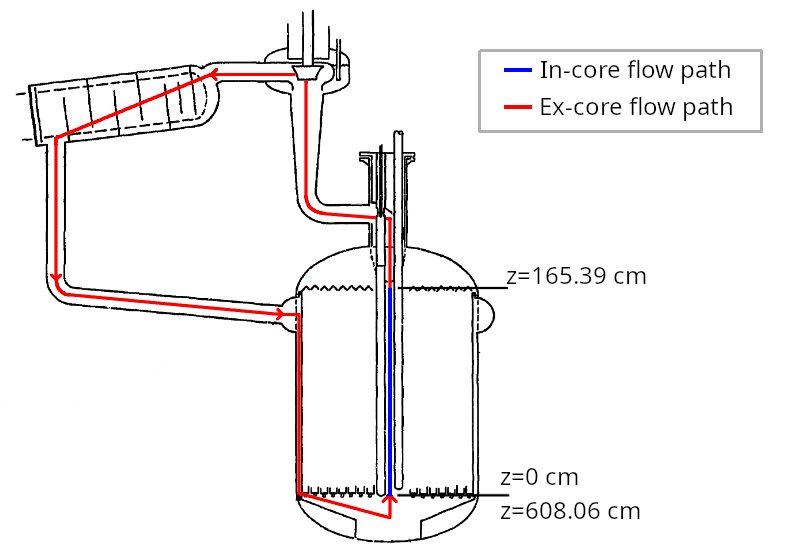
\includegraphics[width=1\textwidth]{../images/MSRE_loop_drawing_3.png}
    \end{center}
          \caption{The flow path and bounds for the in-core region of the \gls{MSRE}, overlayed on the \gls{MSRE} loop diagram from \cite{engel1970spray}.}
    \label{fig:msreflow}
  \end{figure}
        \end{columns}
\end{frame}
\subsection{Objectives}
\begin{frame}
  \frametitle{This work will capture \gls{MSR} phenomena in the \gls{DNP} groups}
        \textbf{The primary objective of this work is to generate improved \gls{DNP} group parameters for \glspl{MSR}.}

        \begin{block}{The objectives of this work are to:}
            \begin{itemize}
		    \item \progressbar[filledcolor=green]{0.75} Create a Python package (\gls{MoSDeN}) for \gls{DNP} group parameter generation
                \item \progressbar[filledcolor=yellow]{0.5} Verify and validate the improved \gls{DNP} group parameters
                \item \progressbar[filledcolor=red]{0.1} Evaluate the impact of these improved parameters on transient simulations for safety, security, and safeguards problems
            \end{itemize}
        \end{block}

\end{frame}

\section{Background}
\subsection{DNP Groups}
\begin{frame}
  \frametitle{Two approaches can acquire the delayed neutron count rate}
  %\frametitle{There are two approaches to calculating \gls{DNP} group parameters}
    \begin{block}{\gls{DNP} group parameter calculation follows the following steps:}
        \begin{enumerate}
            \item Irradiate a fissile sample
            \item Measure/calculate a delayed neutron count rate
            \item Determine the \gls{DNP} group parameters that best fit that count rate
        \end{enumerate}

    \vspace{2mm}
    \textbf{The specific steps depend on which approach is used.}

    \end{block}
        \begin{columns}
                \column[t]{0.45\textwidth}
                \begin{block}{Macroscopic approach}
                    The delayed neutron count rate is \textit{measured}.
                \end{block}
                \column[t]{0.45\textwidth}
                \begin{block}{Microscopic approach}
                    The delayed neutron count rate is \textit{calculated}.
                \end{block}
        \end{columns}

\end{frame}

\begin{frame}
  \frametitle{The macroscopic approach irradiates a sample physically}
  The delayed neutron count rate is directly measured after sample irradiation.

  \begin{figure}[htbp!]
    \begin{center}
      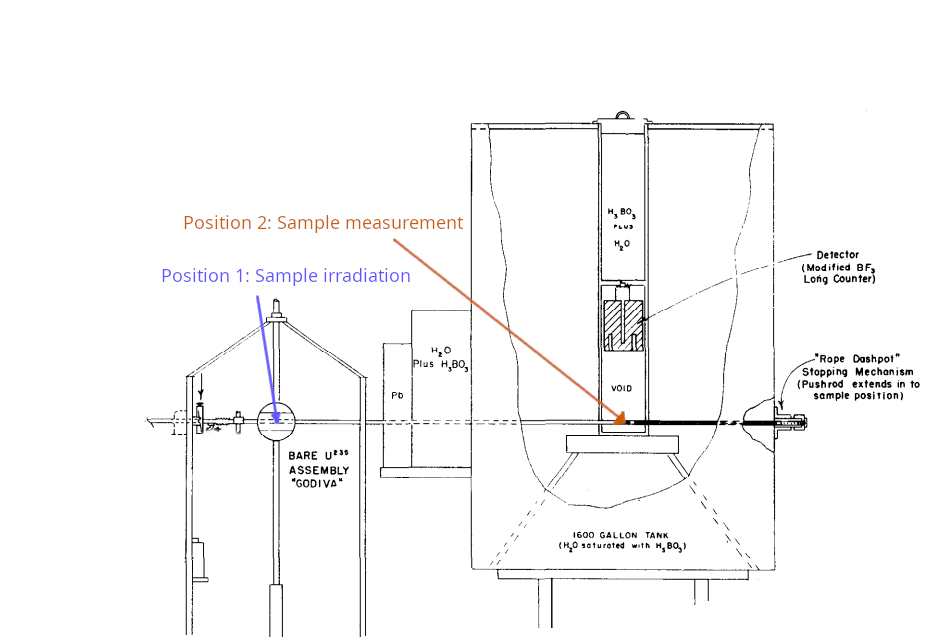
\includegraphics[width=0.6\textwidth]{../images/keepin-setup-mod.png}
    \end{center}
    \caption{Simplified experimental setup for measuring delayed neutron emission from irradiation of a 3 gram sample in Godiva referenced from \cite{keepin1957delayed}.}
    \label{fig:keepin-setup}
  \end{figure}
\end{frame}
\begin{frame}
  \frametitle{The microscopic approach irradiates a sample computationally}
    \begin{block}{\gls{DNP} group formulation follows the following steps:}
        \begin{enumerate}
            \item Irradiate a fissile sample
            \item Measure/calculate a delayed neutron count rate
            \item Determine the \gls{DNP} groups that best fit that count rate
        \end{enumerate}
    \textbf{The specific steps depend on which approach is used.}
    \end{block}
\end{frame}
\begin{frame}
  \frametitle{There are two common irradiation types used to generate groups}
  The $I$ \glspl{DNP} are condensed into $K$ groups.
  \begin{equation}
    \dot{n}_{d}(t) = \sum_{i}^{I} P_{n, i} \lambda_i N_i(t)
    \label{eq:dnpsingleeq}
  \end{equation}
    \begin{columns}
            \column[t]{0.45\textwidth}
            \begin{block}{Pulse irradiation}
                \begin{equation}
                \dot{n}_d(t) \approx F_s \sum_{k=1}^{K}  \bar{\nu}_{d, k} \lambda_k e^{-\lambda_k t}
                \label{eq:delnu-fit}
                \end{equation}
            \end{block}
            \column[t]{0.45\textwidth}
            \begin{block}{Saturation irradiation}
                \begin{equation}
                \dot{n}_d(t) \approx \dot{F}_s \sum_{k=1}^{K}  \bar{\nu}_{d, k} e^{-\lambda_k t}
                \label{eq:delnu-fit-sat}
                \end{equation}
            \end{block}
    \end{columns}
    \vspace{2mm}
    \textbf{The \gls{DNP} parameters $\bar{\nu}_{d,k}$ and $\lambda_k$ make $\dot{n}_d(t)$ match using exponential peeling \cite{brunson1955measurement, keepin1955delayed}, least squares \cite{brady1988evaluation, keepin1957delayed}, or half-lives of specific \glspl{DNP} \cite{saphier1977evaluated}.}
\end{frame}
\subsection{MSR Phenomena}
\begin{frame}
  \frametitle{Fuel salt recirculation affects concentration of \glspl{DNP}}
        \begin{columns}
                \column[t]{5cm}
                
                \begin{block}{In-core and ex-core salt circulation can be modeled using:}
                    \begin{itemize}
                        \item Explicit modeling
                        \item Scaled flux method \cite{betzler_liquid-fueled_2021}
                    \end{itemize}
                \end{block}

                The scaled flux method is generally accurate for spatially averaged concentrations \cite{seifert_luke_computationally_2025}.
                \vspace{2mm}

                \textbf{For a circulating fissile sample, the scaled flux method may not be sufficient.}

                \column[t]{5cm}
        \begin{figure}[htbp!]
        \begin{center}
        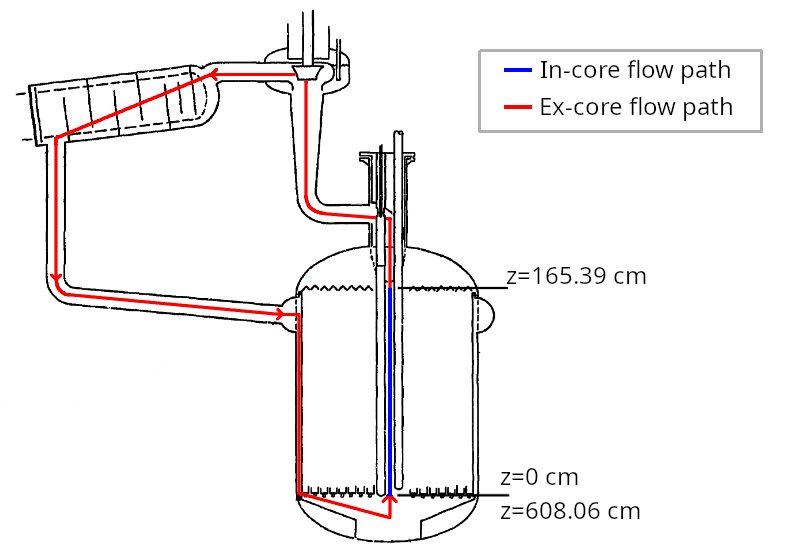
\includegraphics[width=1\textwidth]{../images/MSRE_loop_drawing_3.png}
        \end{center}
            \caption{The flow path and bounds for the in-core region of the \gls{MSRE}, overlayed on the \gls{MSRE} loop diagram from \cite{engel1970spray}.}
        \label{fig:msreflow}
        \end{figure}
  
        \end{columns}
\end{frame}
%\begin{frame}
  \frametitle{The scaled flux method simplifies recirculation modeling}

\begin{block}{The scaled flux method:}
    \begin{itemize}
        \item Scales the flux by the fraction of time the salt is in the core
        \item Reduces cost compared to spatial tracking
        \item Reduces cost compared to a piecewise approach
        \item Is accurate when the concentration is averaged spatially \cite{seifert_luke_computationally_2025}
    \end{itemize}
\end{block}

\textbf{The method may not be accurate for a minutes-long irradiation of a heterogeneous sample.}
\end{frame}
\begin{frame}
	\frametitle{Chemical reprocessing should affect \gls{DNP} groups}
	\begin{block}{Online chemical reprocessing includes:}
	\begin{itemize}
		\item Fission product removal
		\item Fresh fuel addition
	\end{itemize}
	\end{block}

	Existing \gls{DNP} group parameters do not account for these effects.
	\vspace{2mm}

	\textbf{For example, a reprocessing scheme with 100\% of all \glspl{DNP} chemically removed should \textit{not} have the same \gls{DNP} groups.}
\end{frame}

%\subsection{Safety, Security, and Safeguards}
\section{Methodology}
\subsection{MoSDeN Overview}
\begin{frame}
	\frametitle{MoSDeN generates improved \gls{DNP} group parameters}
	\Gls{MoSDeN} is an open-source Python package in development that will enable users to generate improved \gls{DNP} group parameters.
	\begin{block}{MoSDeN currently enables:}
		\begin{itemize}
			\item Use of various data inputs for half-lives ($\tau$), emission probabilities ($P_n$), and cumulative fission yields (CFY)
			\begin{itemize}
				\item ENDF-6 formatted data
				\item OpenMC chain data
				\item Custom data
			\end{itemize}
			\item The microscopic approach using the 0D scaled model
			\begin{itemize}
				\item Equilibrium approximated
				\item Scaled flux method
				\item Non-linear least squares
				\item Generic fissile nuclide
				\item Generic neutron irradiation energy
			\end{itemize}
		\end{itemize}
	\end{block}

	\textbf{\Gls{MoSDeN} currently offers the 0D scaled model, which only enables saturation irradiations to be modeled.} 

	%\textbf{The MoSDeN package is in development and offers improved \gls{DNP} group generation for \glspl{MSR} on a per-problem basis.}
\end{frame}

\begin{frame}
  \frametitle{The saturation irradiation is a non-linear least squares problem}
  \textbf{The group parameters are calculated by equating the delayed neutron count rates.}

  \begin{equation}
    \dot{F}_s \sum_{k=1}^{K}  \bar{\nu}_{d, k} e^{-\lambda_k t} \approx \sum_{i}^{I} P_{n, i} \lambda_i N_i(t)
  \end{equation}

    \begin{equation}
        A \vec{x} \approx \vec{b}
    \end{equation}

    \begin{equation}
    \dot{F_s}
    \begin{bmatrix}
    e^{-\lambda_1 t_0} & \hdots &  e^{-\lambda_K t_0}\\
    \vdots                                     & \ddots &  \vdots                      \\
    e^{-\lambda_1 t_m} &  \hdots  & e^{-\lambda_K t_m}\\
    \end{bmatrix}
    \begin{bmatrix}
    \bar{\nu}_{d, 1}\\
    \vdots\\
    \bar{\nu}_{d, K}\\
    \end{bmatrix}
    \approx
    \begin{bmatrix}
    \dot{n}_d(t_0)  \\
    \vdots\\
    \dot{n}_d(t_m)\\
    \end{bmatrix}
    \label{eq:lambda}
    \end{equation}

\end{frame}
\begin{frame}
  \frametitle{The residual minimizes the difference between delayed neutron count rates}
  \begin{equation}
    r = \min_x \left| \left| \frac{\textcolor{blue}{\vec{b}} - \textcolor{orange}{A} \textcolor{olive}{\vec{x}}}{\textcolor{blue}{\vec{b}}} \right| \right|_2^2,
  \end{equation}
  where
  \begin{align}
    \tau_k &\in [1\; ms, 1000 \;s] \nonumber \\
    \bar{\nu}_{d,k} & \in [0, 1] \nonumber.
  \end{align}

  \textbf{\gls{MoSDeN} uses the SciPy package's optimize module to solve this non-linear least squares problem \cite{scipy}.}

\end{frame}
\begin{frame}
  \frametitle{Uncertainties are tracked using Monte Carlo sampling}
  \begin{block}{The process for uncertainty tracking is as follows:}
    \begin{enumerate}
        \item Normally sample $P_{n,i}$, $\tau_i$, and $N_i(t)$ within their uncertainties for every \gls{DNP}
        \item Calculate the \gls{DNP} group parameters using non-linear least squares
        \item Record the results and repeat
    \end{enumerate}
  \end{block}

  \begin{block}{After all simulations finish:}
    \begin{enumerate}
        \item Groups are defined based on half-lives (e.g. longest lived half-life and yield are group one)
        \item The mean values and standard deviations are calculated
    \end{enumerate}
  \end{block}

\end{frame}
\begin{frame}
  \frametitle{\Gls{MoSDeN} uses a newly-derived form of the group fit for \glspl{MSR}}
  Assuming the sample experiences a square-wave power history during in-core and ex-core times, an \gls{MSR} specific group fit equation can be derived.



\begin{align}
\frac{F(\tau)}{F_0} =& \sum_{j=0}^{J} H(\tau - j\cdot \tau_{net}) - H(\tau - j \cdot\tau_{net} -\tau_{in})
\intertext{where}
F(\tau) =& \mbox{ the fission rate history [$\frac{\#}{s}$].} \nonumber \\
H =& \text{ the Heaviside function [-]} \nonumber \\
\tau_{net} =& \;\tau_{in} + \tau_{ex} \nonumber \\
=& \text{ the total time per circulation [$s$]} \nonumber \\
J =& \left\lfloor \frac{T}{\tau_{net}} \right\rfloor \nonumber \\
  =& \text{ the number of recirculations [$\#$]} \nonumber \\
F_0 =& \text{ the magnitude of the constant fission rate [$\frac{\#}{s}$].} \nonumber
\end{align}

\end{frame}


\subsection{0D Scaled Model}
\begin{frame}
  \frametitle{The 0D scaled model is implemented in MoSDeN}
  \textbf{MoSDeN uses simulation parameters and external data to generate improved \gls{DNP} parameters.}

  \begin{figure}[H]
    \centering
    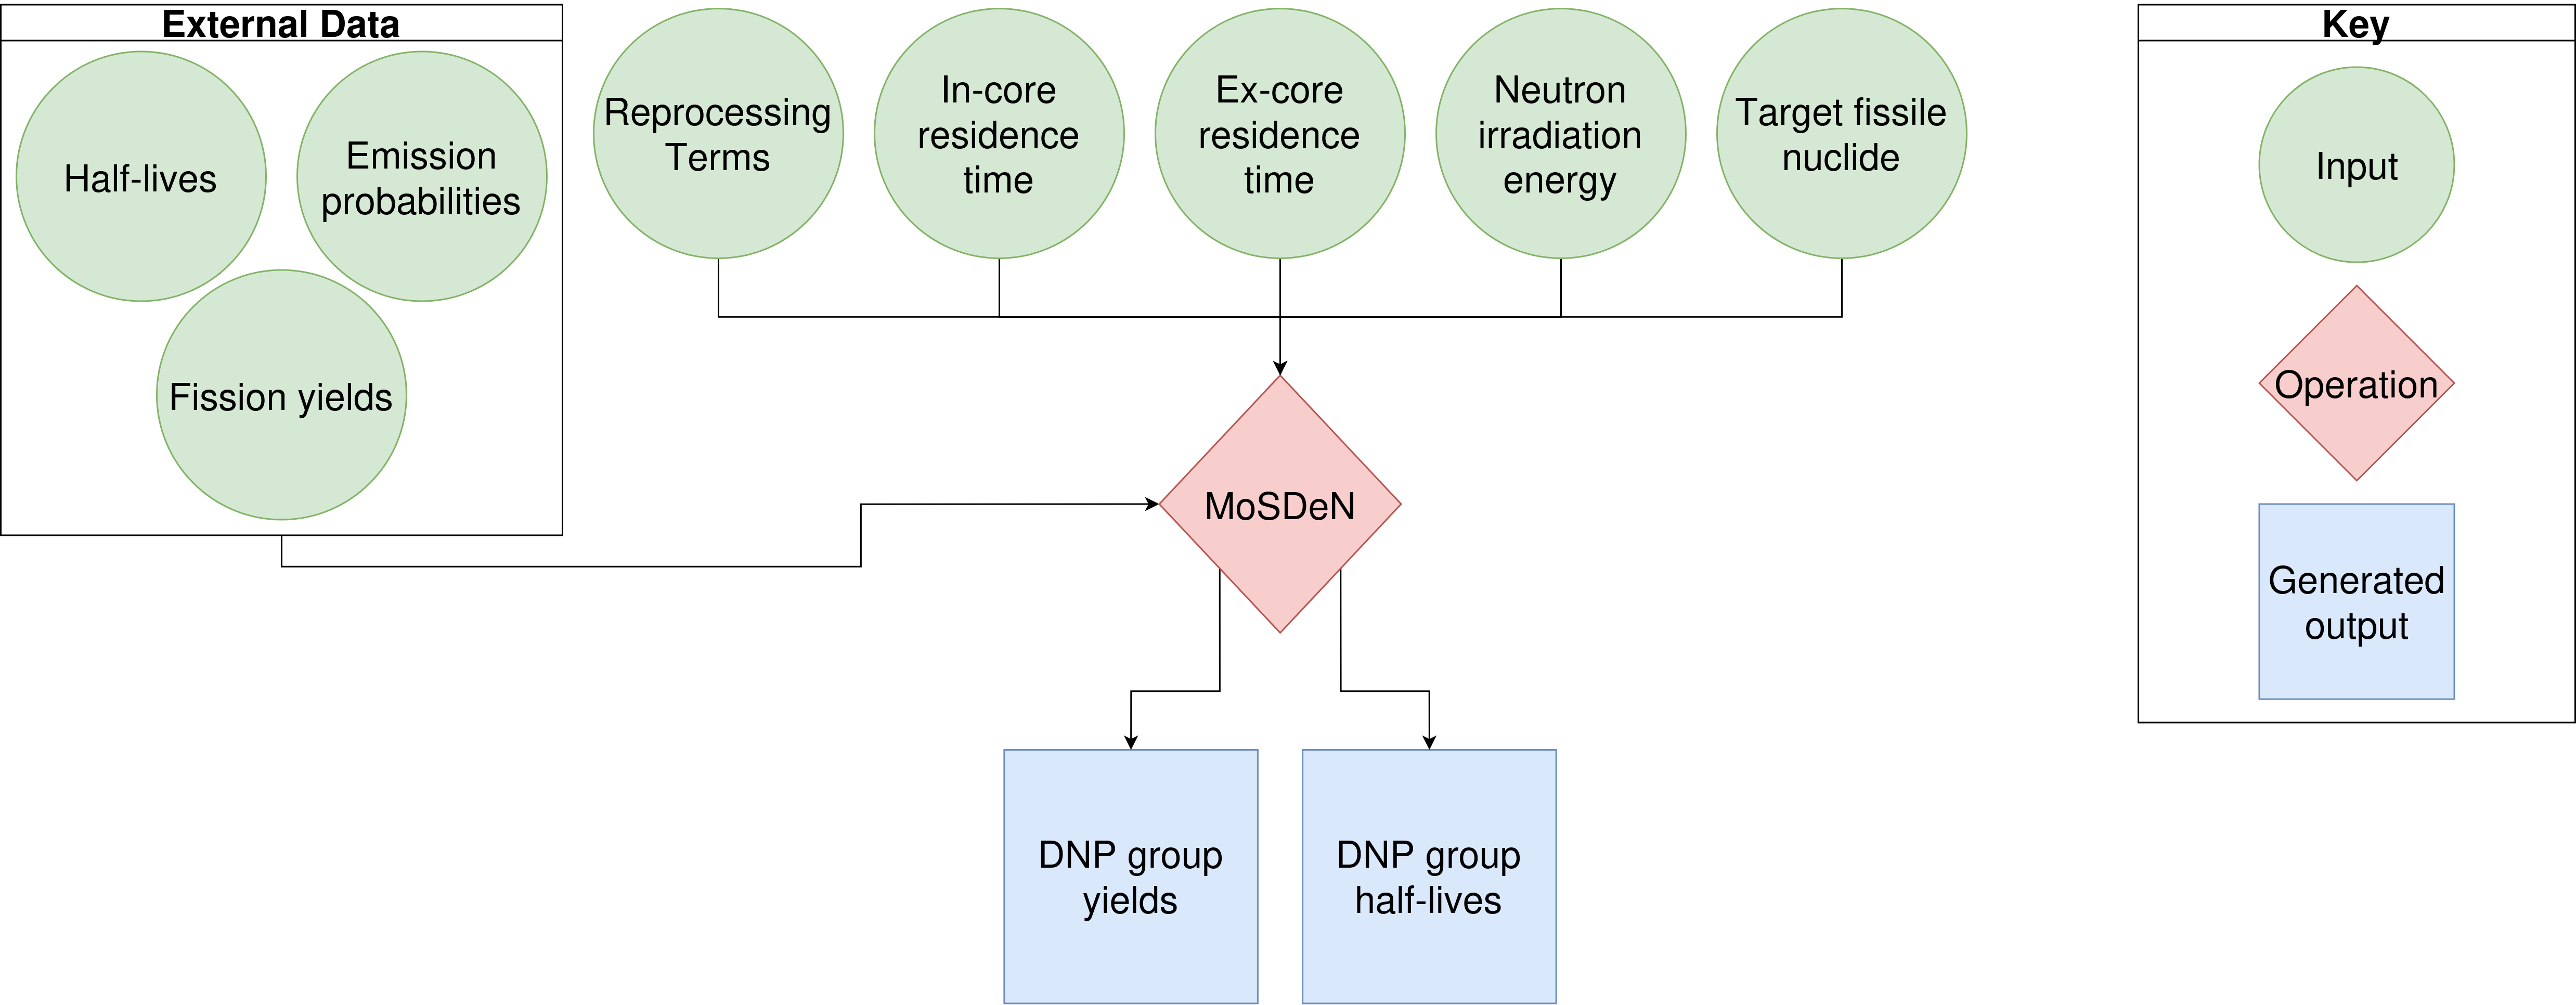
\includegraphics[width=1\textwidth]{../images/data-driven-large.png}
    \caption{Flow diagram of 0D scaled model used to generate improved \gls{DNP} group parameters.}
    \label{fig:data-model}
  \end{figure}
\end{frame}
\begin{frame}
  \frametitle{The 0D scaled model is fast but uses many approximations}
    The equilibrium concentration of each \gls{DNP} is calculated for the 0D scaled model as \cite{huynh2014calculation}:

    \begin{equation}
        N_i = \frac{f_{in} CFY_i}{\lambda_i},
        \label{eq:cfy-conc}
    \end{equation}
    where
    \begin{align}
        f_{in} &= \text{the fraction of time fuel-salt spends in the core [-]} \nonumber \\
        CFY_{i} &= \text{the cumulative fission yield of nuclide $i$ [-].} \nonumber
    \end{align}

    \begin{block}{The limitations of the 0D model include:}
        \begin{itemize}
            \item Concentration calculation does not include cross sections
            \item The concentration is only available at equilibrium
            \item The depletion chain is not tracked, so chemical removal is underestimated
        \end{itemize}
    
    \end{block}

\end{frame}
\section{Preliminary Results}
\begin{frame}
    \frametitle{The parameters for the 0D scaled model analyses}

    \begin{table}[]
    \centering
    \caption{Default parameters for 0D scaled model simulations.}
    \begin{tabular}{lrl}
        \hline
        Parameter & Value & Units\\
        \hline
        \rule{0pt}{2ex}\vspace{0.1 mm}Fissile Nuclide & \vspace{0.1 mm}$^{235}$U & [-]\\
        Incident Neutron Energy & $0.0253$ &$ [eV]$\\
        Fission Yields & ENDF/B-VII.1 \cite{chadwick2011endf} & [-]\\
        Half-lives & IAEA \cite{DIMITRIOU2021144} & [-]\\
        Emission Probability & IAEA \cite{DIMITRIOU2021144} & [-]\\
        Final Decay Time & $1200$ & $[s]$\\
        Decay Time Spacing & Logarithmic & [-]\\
        Decay Time Nodes & 300 & [-]\\
        Sampled Simulations & 1000 & [-]\\
        $\tau_{in}$ & 9 \cite{hanauer1967neutron} & $[s]$\\
        $\tau_{ex}$ & 16 \cite{hanauer1967neutron} & $[s]$\\
        \hline
    \end{tabular}
    \label{tab:default-0dsacled}
\end{table}

\end{frame}
\subsection{Analysis of Yields and Counts}
\begin{frame}
\frametitle{The total delayed neutron yield is dominated by a few DNPs}
\begin{block}{The delayed neutron yield from each \gls{DNP} is given as \cite{huynh2014calculation, mathieu2012new}:}
\begin{equation}
    \bar{\nu}_{d,i} = P_{n, i} CFY_i.
\end{equation}
\end{block}
\begin{figure}[htbp!]
\begin{center}
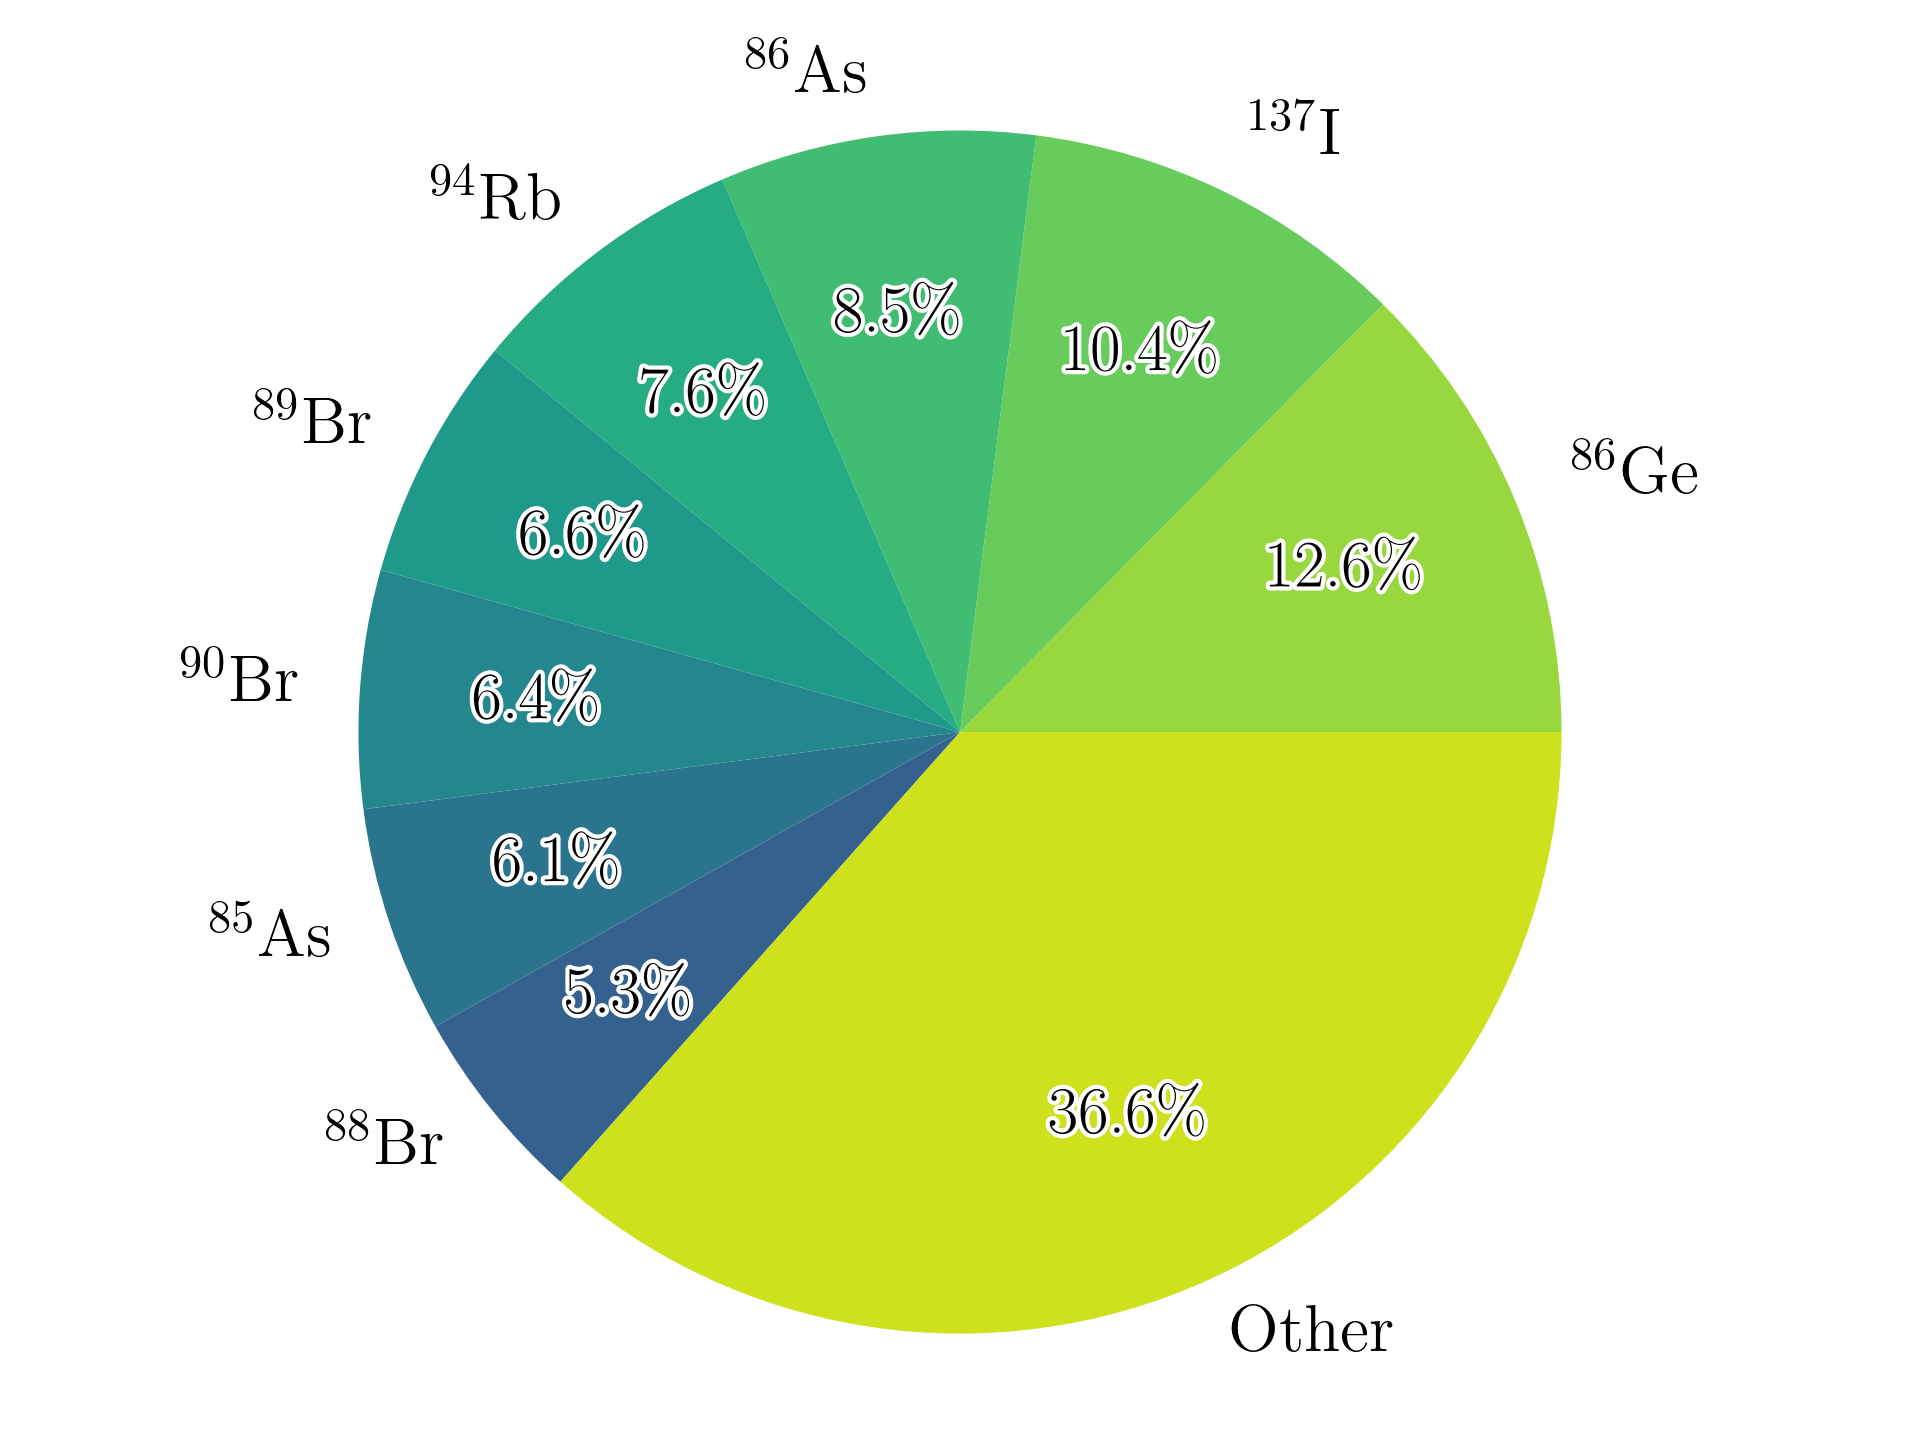
\includegraphics[width=0.6\textwidth]{../images/0dnp_yield.png}
\end{center}
\caption{Relative delayed neutron yield from each \ac{DNP} after a thermal saturation irradiation of $^{235}$U using the 0D scaled model.}
\end{figure}
\end{frame}
\begin{frame}
  \frametitle{The delayed neutron count rate is dominated by a few DNPs}
        \begin{columns}
                \column[t]{0.5\textwidth}
        \begin{figure}[htbp!]
        \begin{center}
        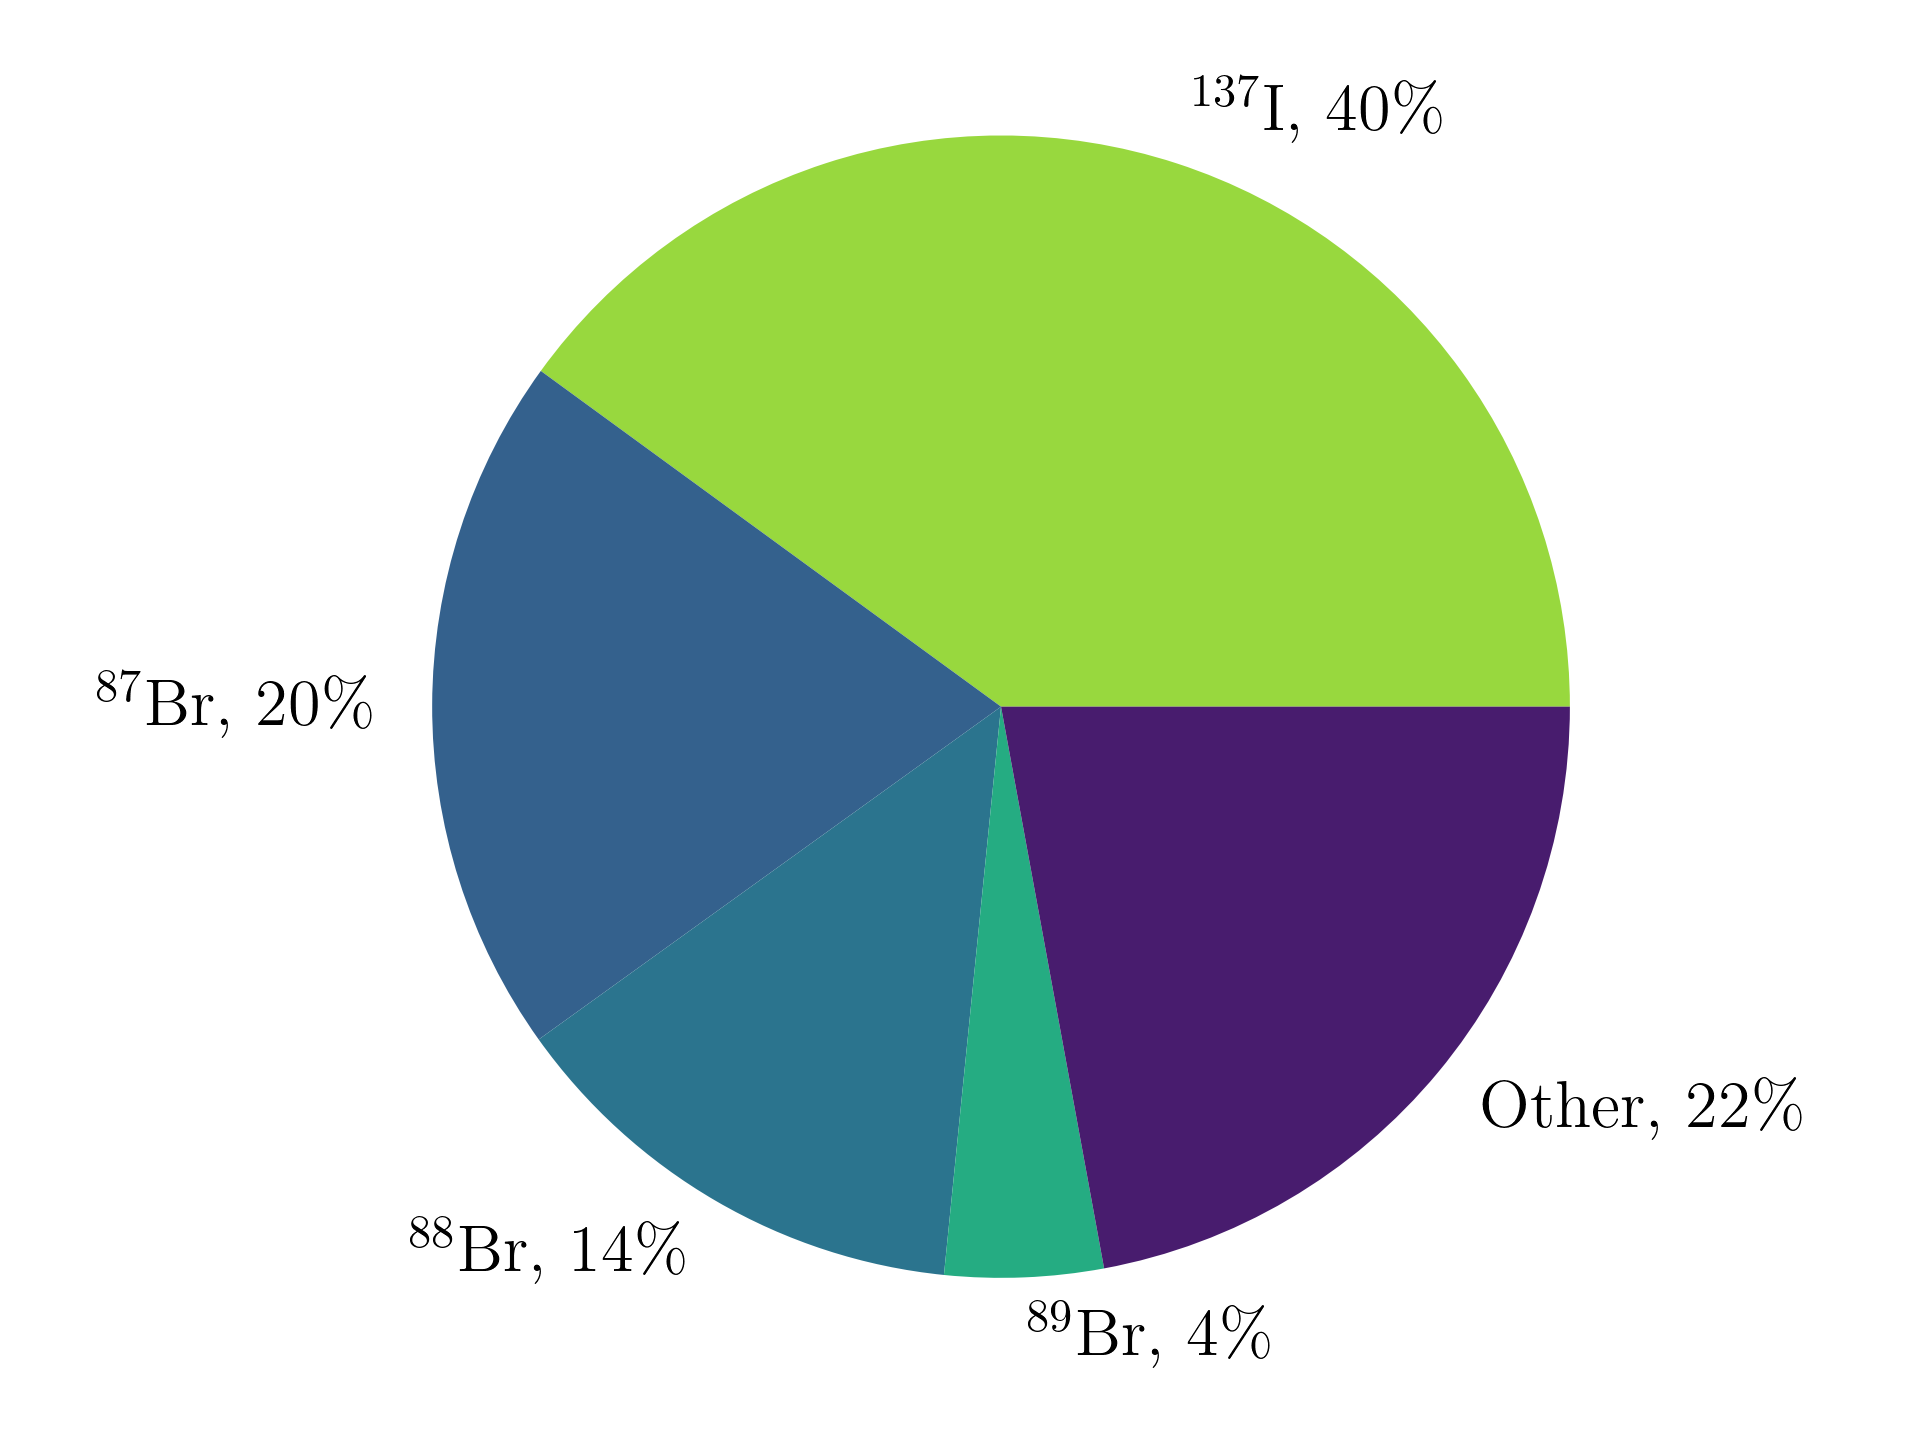
\includegraphics[width=1\textwidth]{../images/1dnp_yield.png}
        \end{center}
            \caption{Relative delayed neutron counts from each \gls{DNP} after a thermal saturation irradiation of $^{235}$U using the 0D scaled model.}
        \end{figure}

                \column[t]{0.5\textwidth}
        \begin{figure}[htbp!]
        \begin{center}
        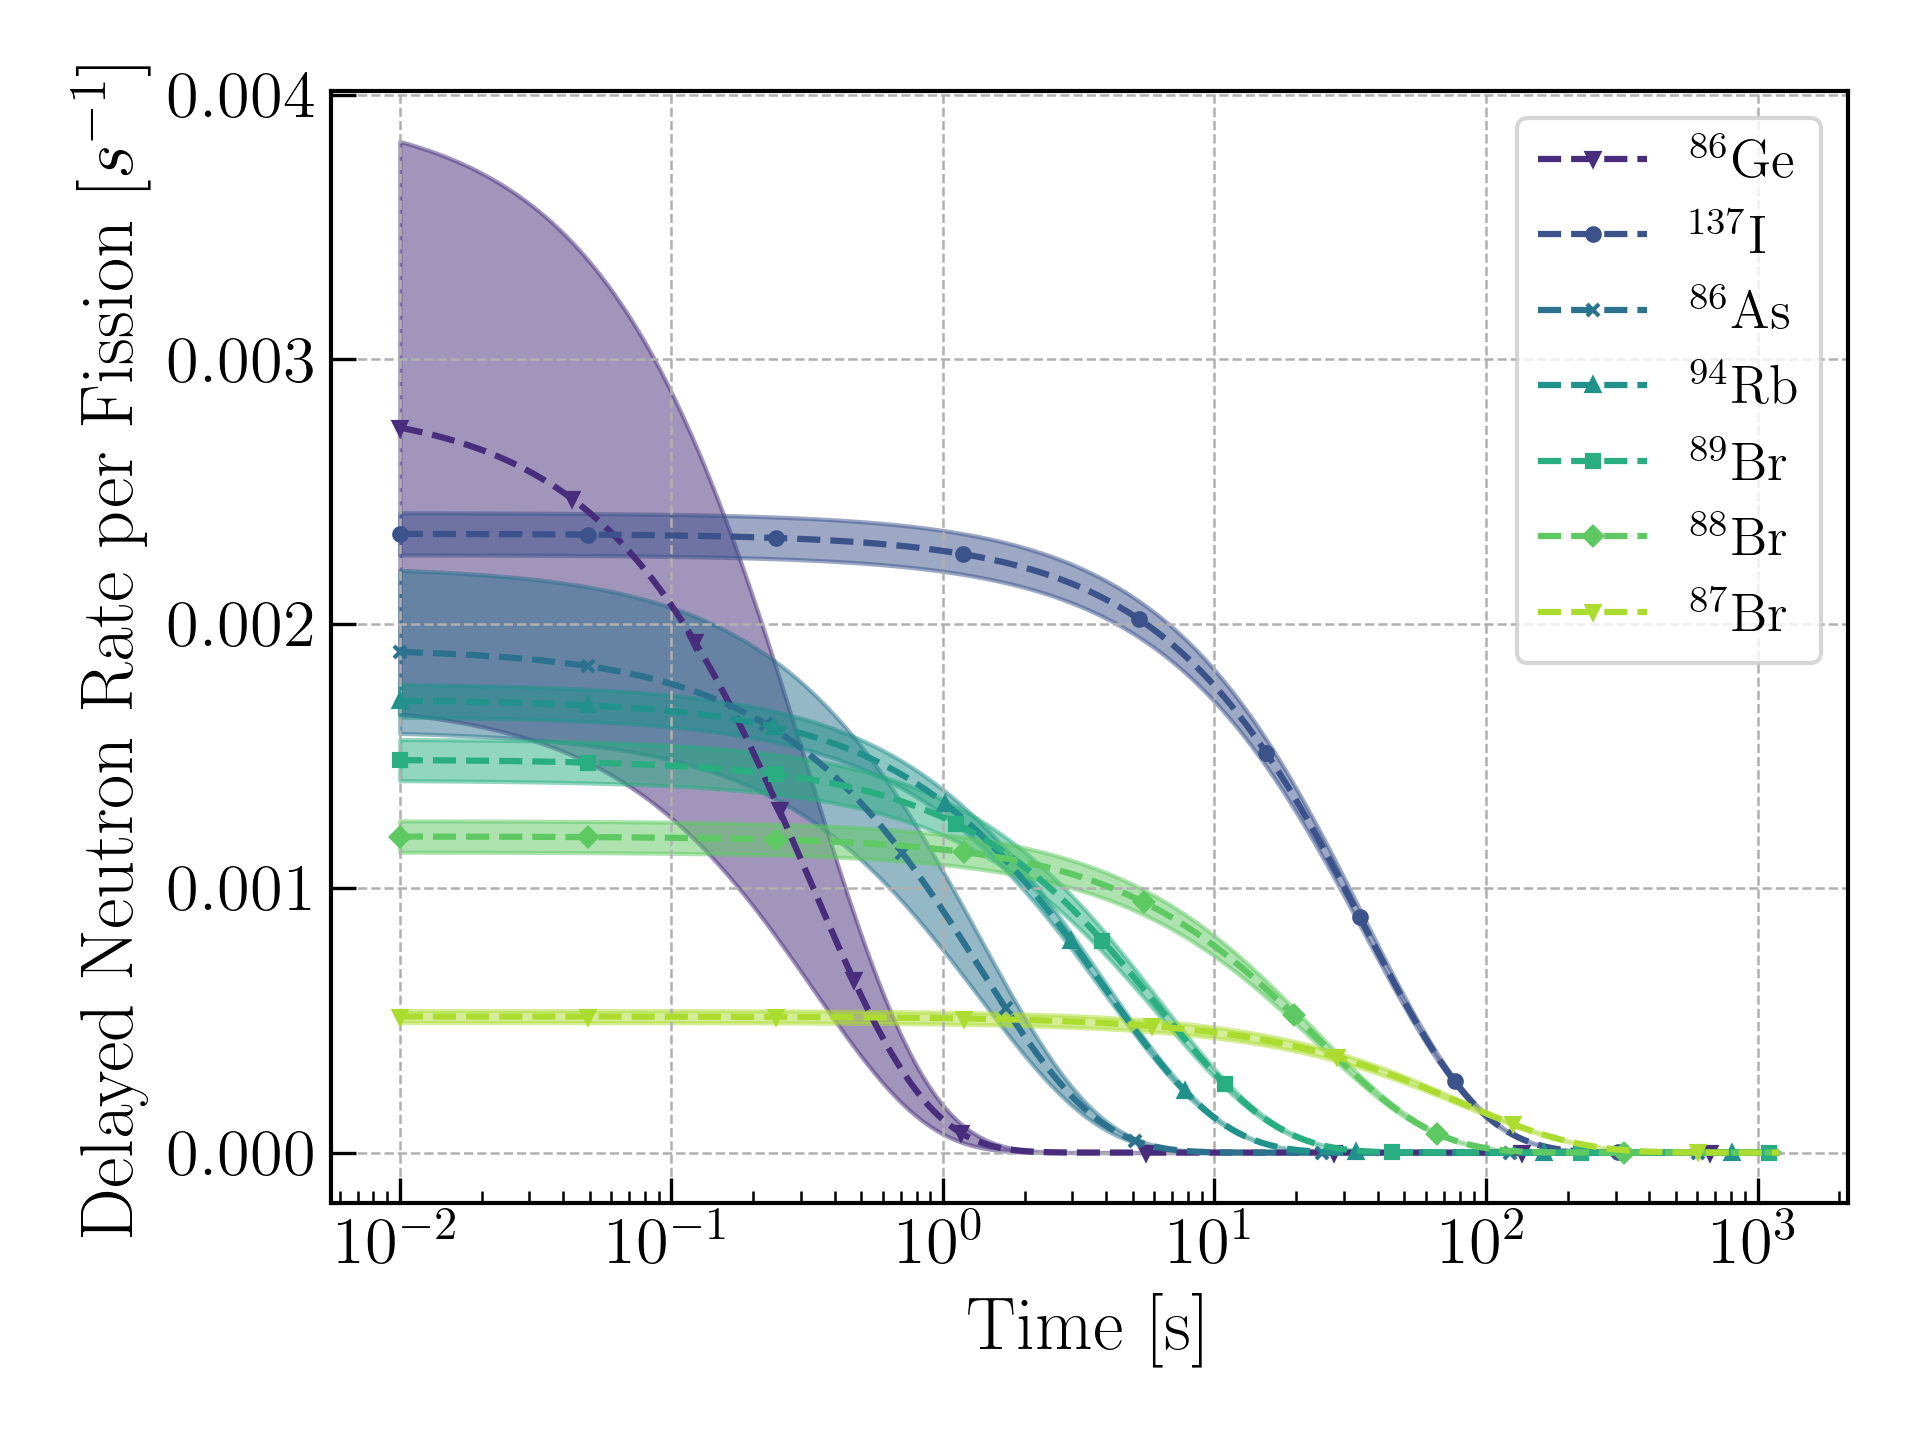
\includegraphics[width=1\textwidth]{../images/individual_nuclide_rates.png}
        \end{center}
            \caption{Relative delayed neutron count rates after a thermal saturation irradiation of $^{235}$U using the 0D scaled model.}
        \end{figure}
        \end{columns}
\end{frame}

\subsection{Sensitivty Studies}
\begin{frame}
  \frametitle{Chemical removal and simulation parameters affect the results}
    \begin{block}{Sensitivity studies of the chemical removal show:}
        \begin{itemize}
            \item Only the noble metal and gas reprocessing groups have a non-negligble impact on \gls{DNP} group parameters
            \item Chemical removal in the 0D scaled model decreases the total delayed neutron yield by 12 $pcm$
        \end{itemize}
    \end{block}
    \begin{block}{Sensitivity studies of the simulation parameters show:}
        \begin{itemize}
            \item Logarithmic time node spacing improves the \gls{DNP} group parameter fit compared to linear spacing with the same number of nodes
            \item Increasing the number of time nodes up to $\approx 800$ improves the results
            \item Increasing the length of time for delayed neutron count data collection up to $\approx 40$ minutes improves results
        \end{itemize}
    \end{block}
\end{frame}
\begin{frame}
  \frametitle{\Glspl{PCC} convey sensitivity of \gls{DNP} group parameters to nuclear data}
  \begin{columns}
    \column[t]{0.45\textwidth}
        \begin{figure}[!ht]
                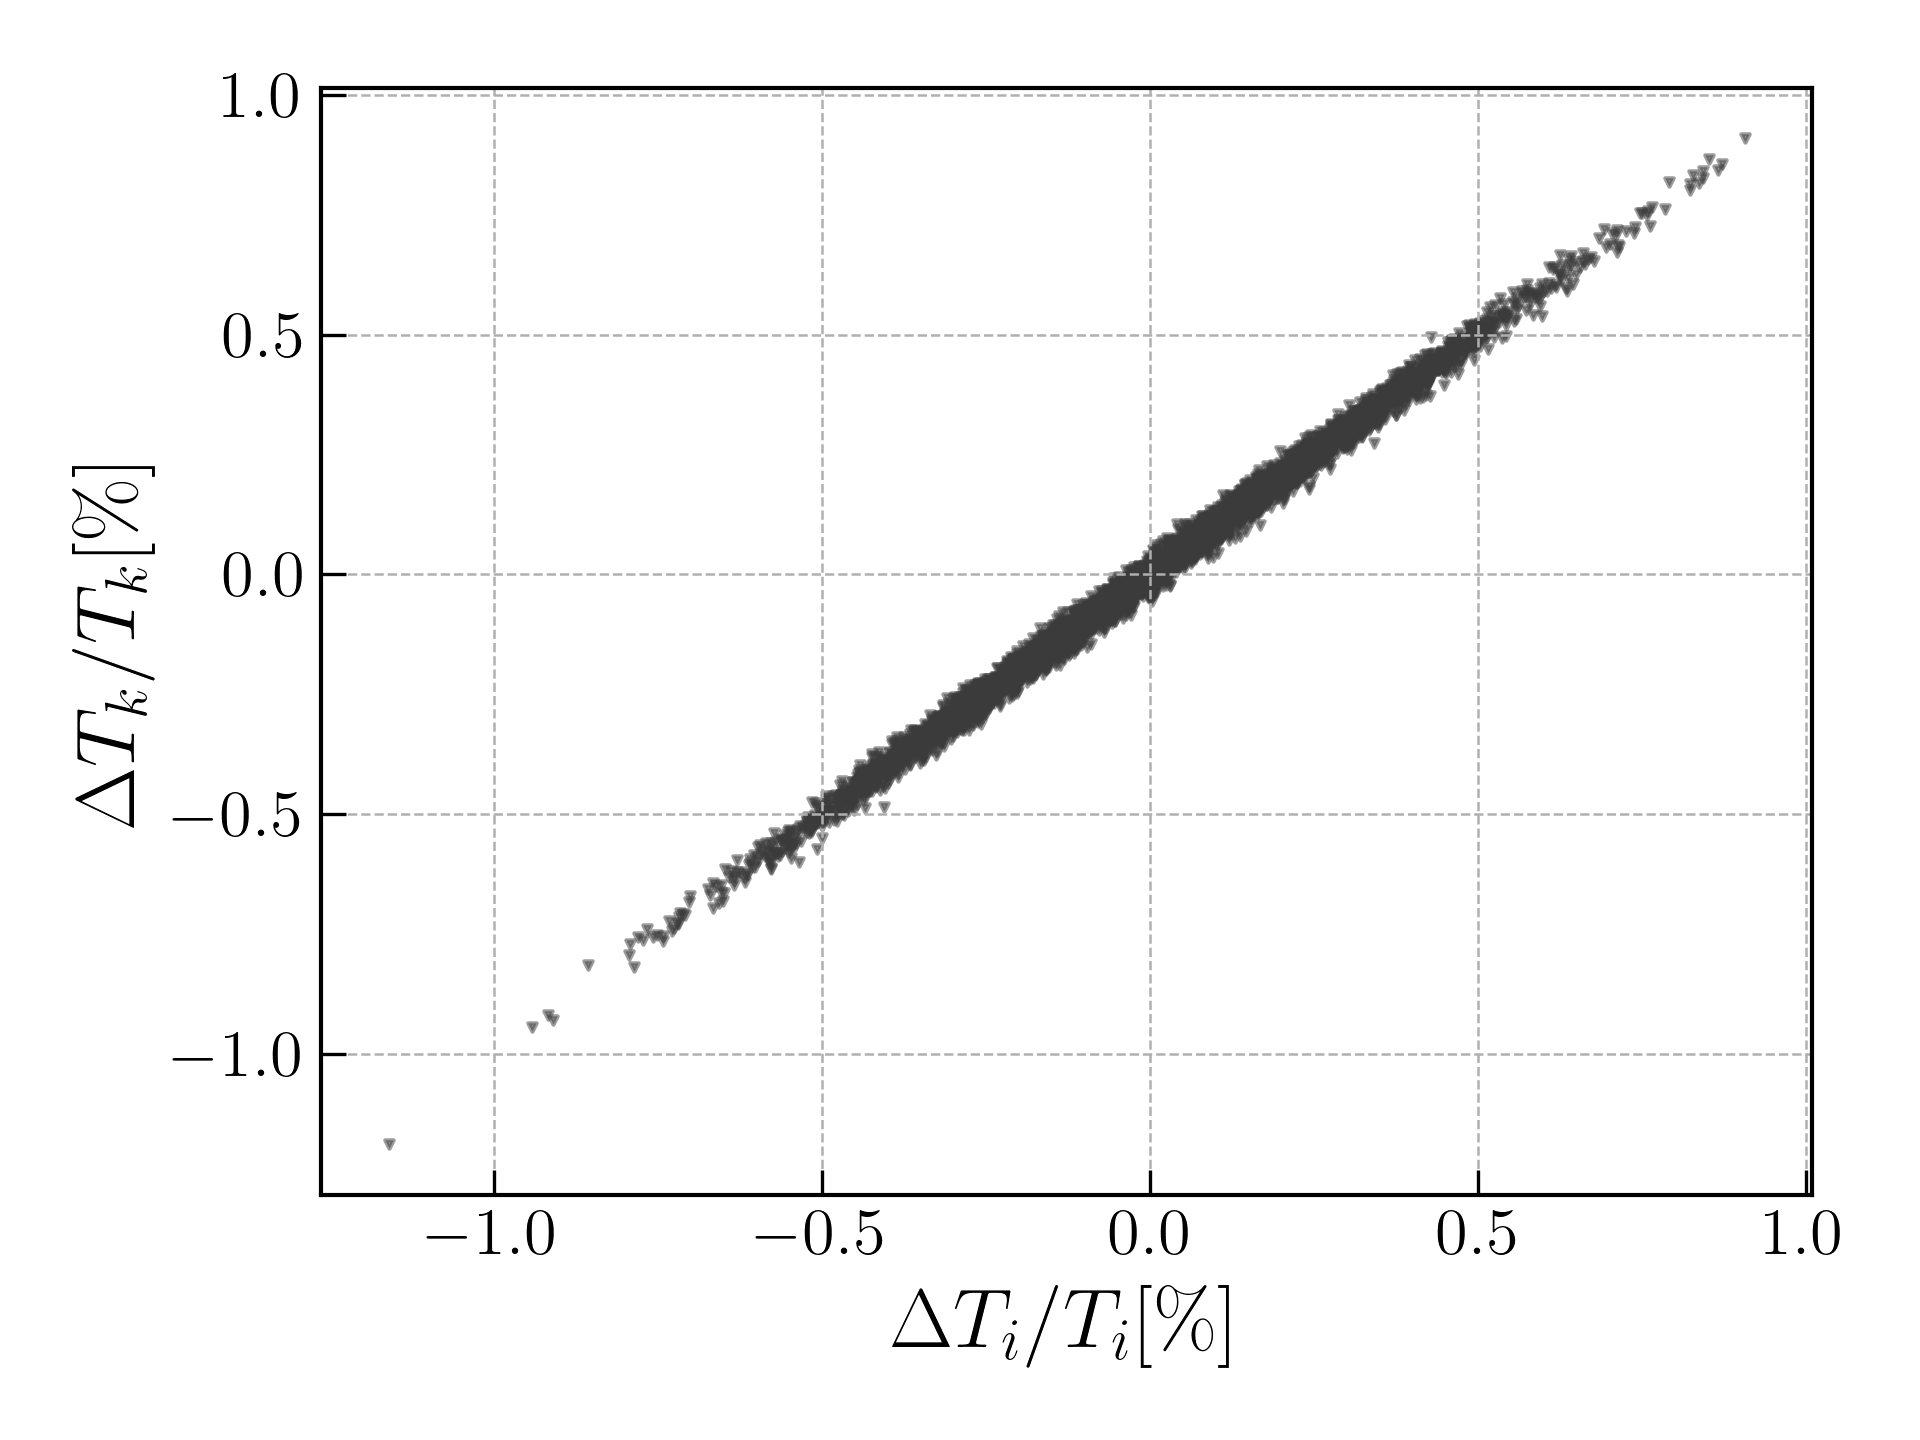
\includegraphics[width=1.0\linewidth]{../images/sens_lam_halflife_Br87_1.png} 
                \caption{\Gls{DNP} group 1 half-life variation due to half-life variation with a \gls{PCC} of 1.00.}
        \end{figure} 
    \column[t]{0.45\textwidth}
        \begin{figure}[!ht]
                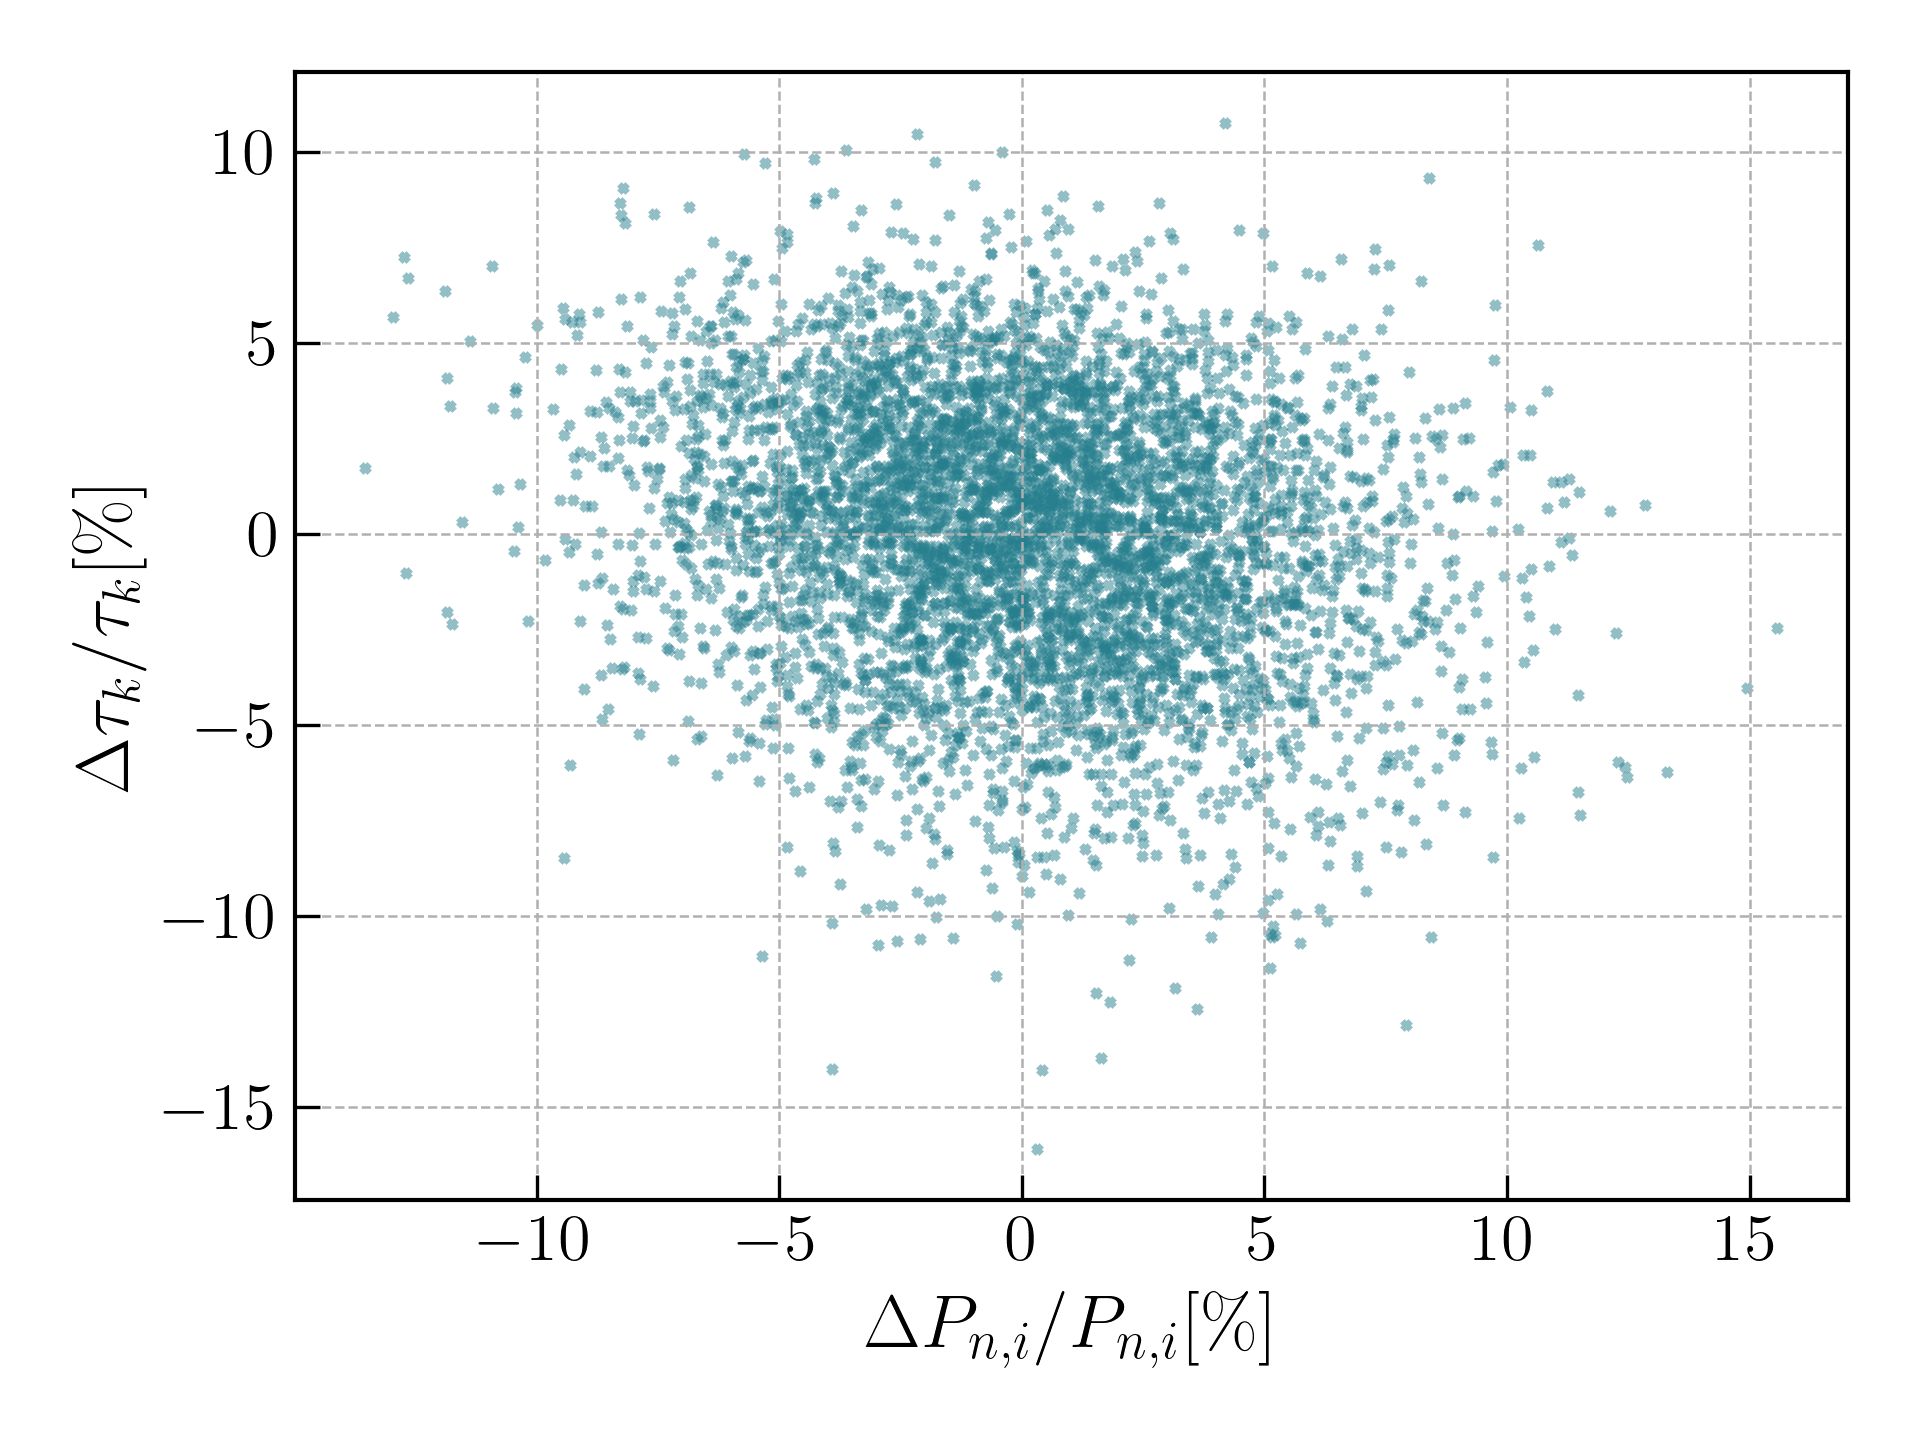
\includegraphics[width=1.0\linewidth]{../images/sens_pn_halflife_Br87_3.png} 
                \caption{\Gls{DNP} group 3 half-life variation due to emission probability variation with a \gls{PCC} of -0.19.}
        \end{figure} 
  
  \end{columns}
  \textbf{The half-life of $^{87}$Br strongly correlates to the group one half-life, while its emission probability does not strongly correlate to the group three half-life.}

\end{frame}


\begin{frame}
  \frametitle{The \gls{PCC} magnitudes show the most sensitive \glspl{DNP}}
  \begin{columns}
    \column[t]{0.67\textwidth}
  \begin{figure}[!ht]
    \centering
    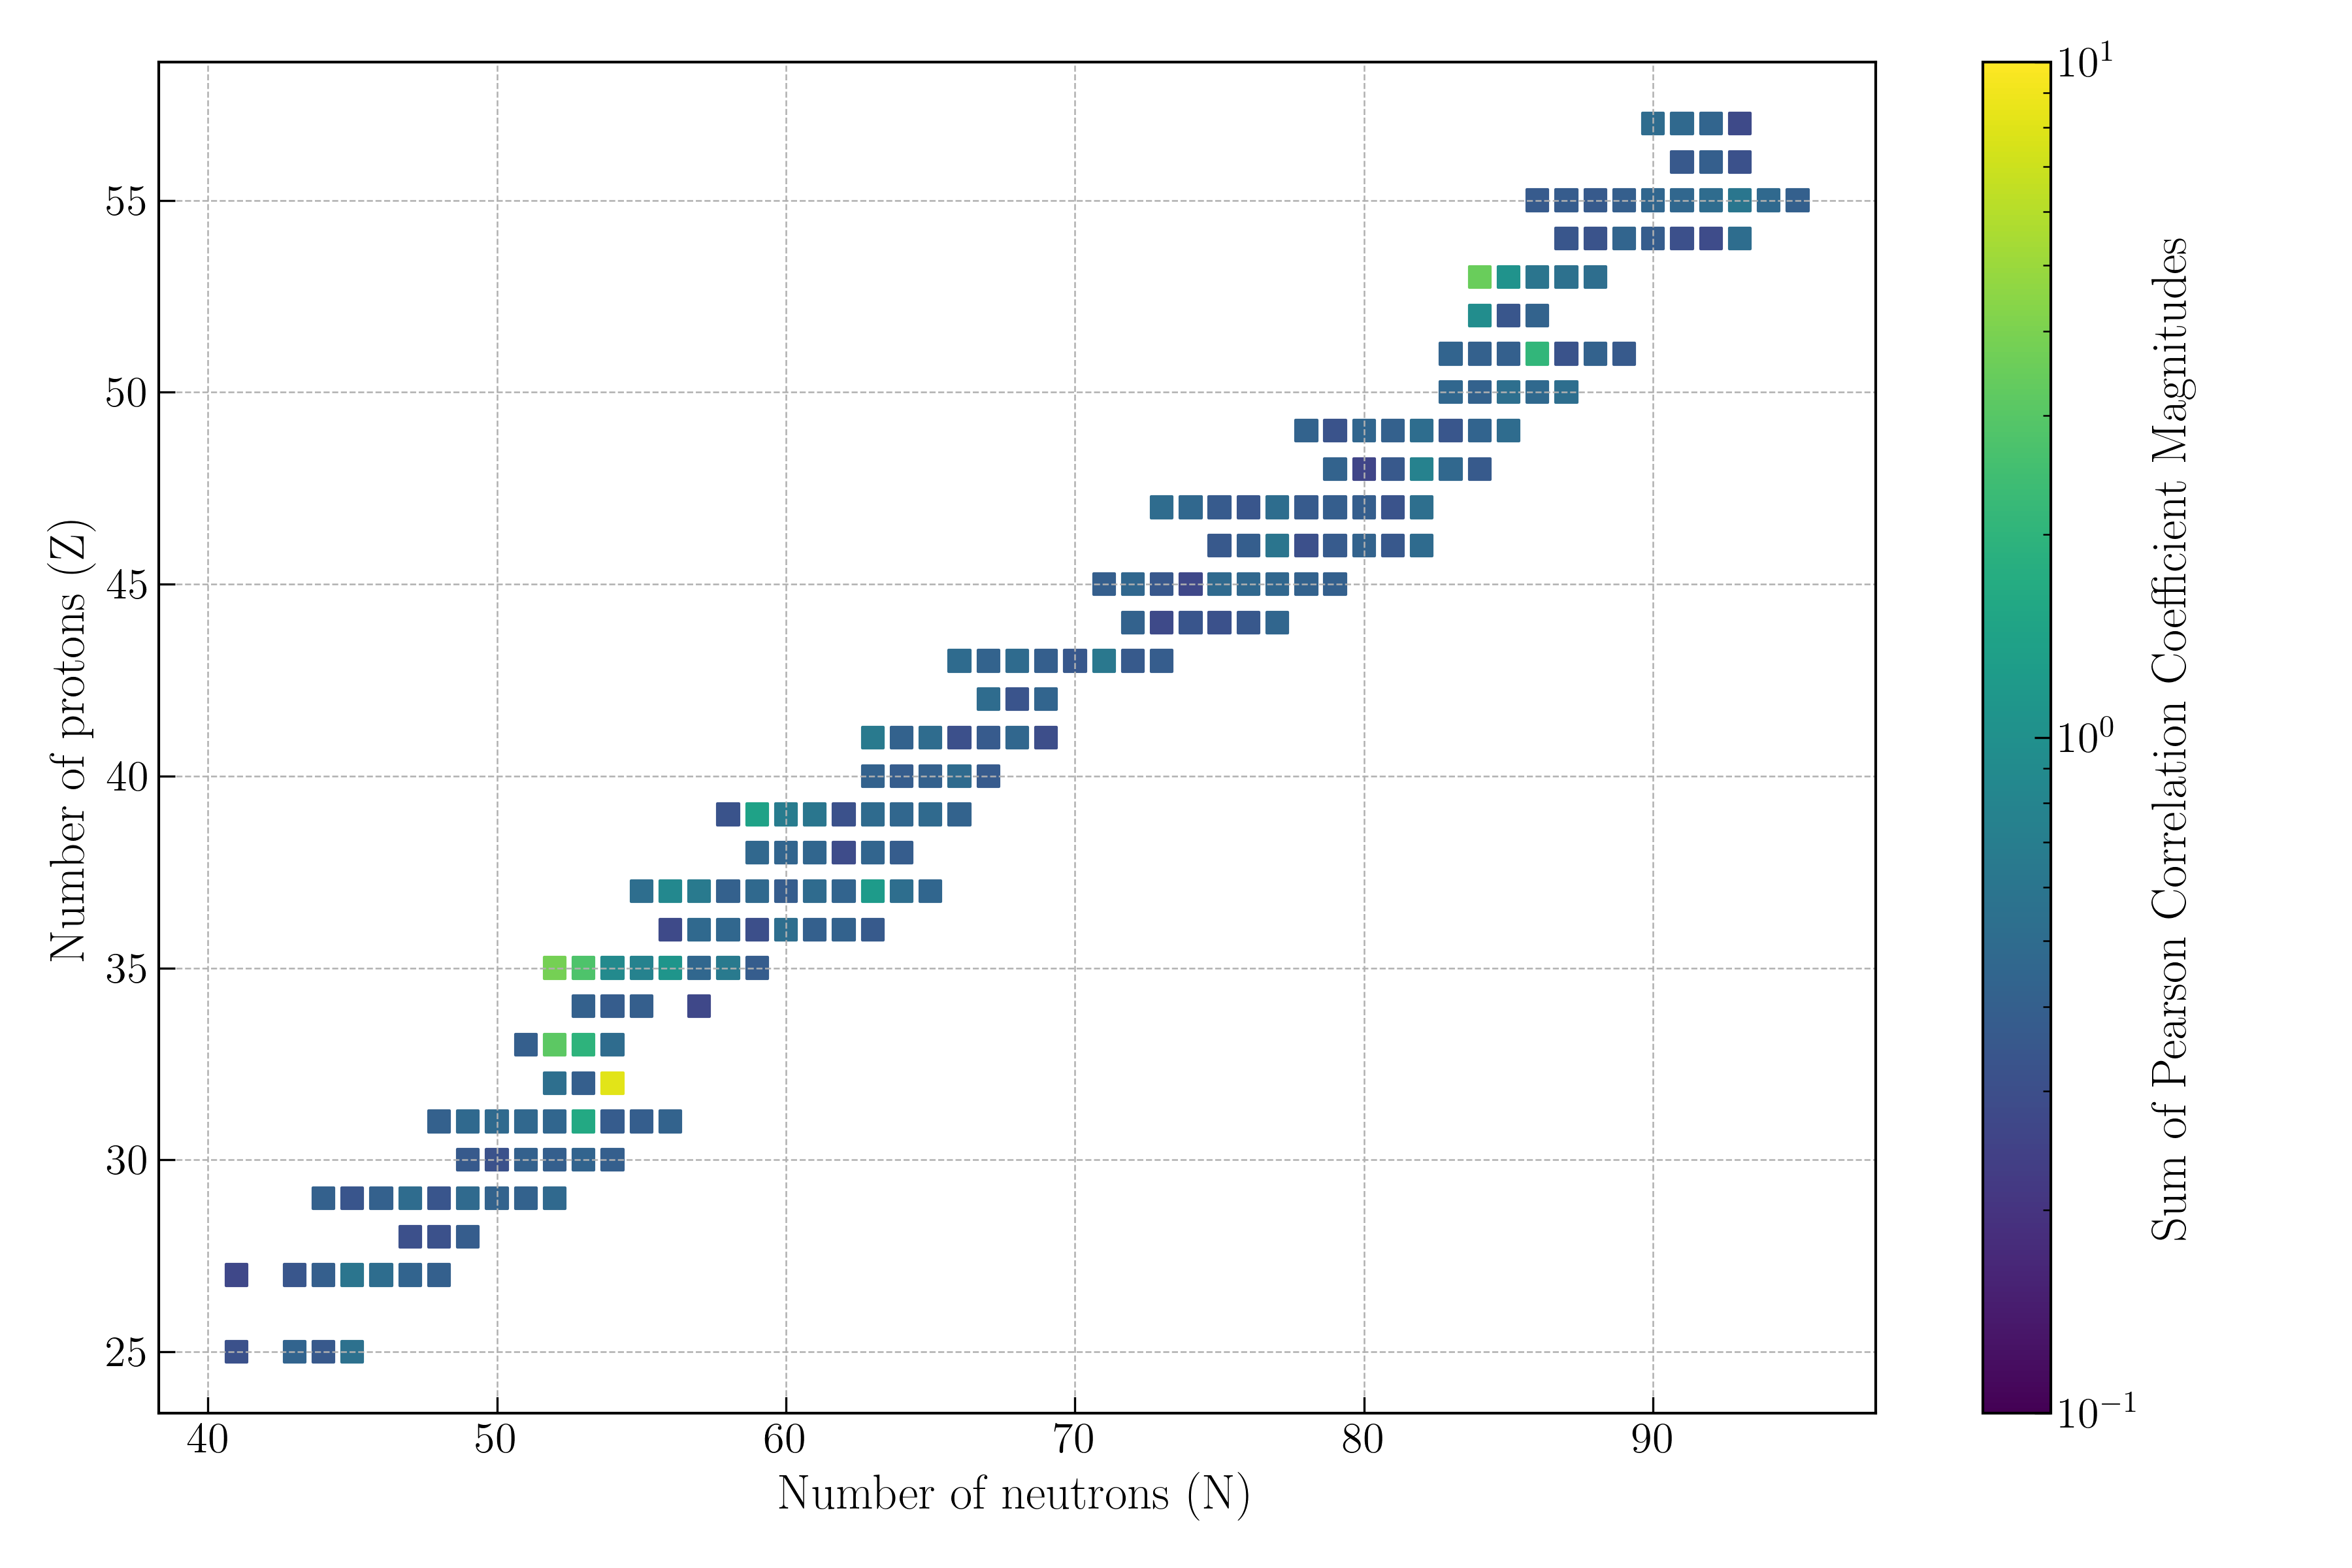
\includegraphics[width=0.95\linewidth]{../images/chart_PCC.png}
    \caption{The summed \gls{PCC} magnitudes after a thermal saturation irradiation of $^{235}$U using the 0D scaled model.}
    \label{fig:summedpccs}
    \end{figure}
    \column[t]{0.33\textwidth}
    \begin{table}[!ht]
    \centering
    \caption{The largest summed \gls{PCC} magnitudes after a thermal saturation irradiation of $^{235}$U using the 0D scaled model.}
\begin{tabular}{lr}
\hline
Nuclide &  $PCC_{i}$ \\
\hline
$^{86}$Ge & 8.06 \\
$^{87}$Br & 3.82 \\
$^{137}$I & 3.52 \\
$^{85}$As & 3.14 \\
$^{88}$Br & 2.77 \\
$^{137}$Sb & 2.08 \\
$^{86}$As & 1.97 \\
$^{84}$Ga & 1.62 \\
$^{98}$Y & 1.42 \\
$^{100}$Rb & 1.22 \\
\hline
\end{tabular}
\label{tab:pcc-summed}
\end{table}
  \end{columns}

\end{frame}


\begin{frame}
  \frametitle{The uncertainty-weighted \gls{PCC} shows critical data needs}
  \begin{columns}
    \column[t]{0.67\textwidth}
    \begin{block}{Uncertainty-weighted PCC $U_i$: }
    \begin{equation}
    U_{i} = \sum_v \frac{\sigma_{i,v}}{x_{i,v}} \sum_g\left|PCC_{i,v,g}\right|,
    \label{eq:Uiv}
\end{equation}
where
\begin{align}
    U_{i,v} &= \text{the uncertainty-weighted sensitivity of }\nonumber \\
    & \text{\;\;\;\;\;\gls{DNP} value $v$ for \gls{DNP} $i$ [-]} \nonumber \\
    \sigma_{i,v} &= \text{the uncertainty in the \gls{DNP} value $v$}\nonumber \\
    & \text{\;\;\;\;\;for \gls{DNP} $i$ [-]} \nonumber \\
    x_{i,v} &= \text{the \gls{DNP} value $v$, representing the half-life,}\nonumber \\
    & \text{\;\;\;\;\;emission probability, or concentration of \gls{DNP} $i$ [-]} \nonumber \\
    PCC_{i, v, g} &= \text{the \gls{PCC} for \gls{DNP} $i$ and value $v$ with}\nonumber \\
    & \text{\;\;\;\;\;\gls{DNP} group parameter $g$ [-].} \nonumber
\end{align}
\end{block}
    \column[t]{0.33\textwidth}
    \begin{table}[!ht]
    \centering
    \caption{The largest summed uncertainty-weighted \gls{PCC} magnitudes after a thermal saturation irradiation of $^{235}$U using the 0D scaled model.}
\begin{tabular}{lr}
\hline
Nuclide &  $U_{i}$ \\
\hline
\textcolor{blue}{$^{86}$Ge} & 1.71 \\
$^{124}$Ag & 0.41 \\
$^{120}$Ag & 0.36 \\
$^{114}$Tc & 0.36 \\
$^{147}$Xe & 0.34 \\
$^{104}$Nb & 0.29 \\
$^{111}$Mo & 0.27 \\
$^{122}$Pd & 0.27 \\
\textcolor{blue}{$^{98}$Y} & 0.26 \\
$^{103}$Zr & 0.26 \\
\hline
\end{tabular}
\label{tab:pcc-summed}
\end{table}
  \end{columns}

\end{frame}


\subsection{Verification}
\begin{frame}
\frametitle{The \gls{DNP} group parameters accurately represent the \gls{DNP} data}
\begin{block}{The total delayed neutron yield ($\bar{\nu}_d$) from the \gls{DNP} group parameters should align with the \gls{DNP} data:}
\begin{equation}
	\sum_{k=1}^{K} \bar{\nu}_{d,k} \approx \sum_{i=1}^I P_{n,i} CFY_i = \bar{\nu}_d
\end{equation}
The $K$ groups give $\bar{\nu}_d = 2.24 \pm 0.13$ per 100 fissions, while the $I$ \glspl{DNP} give $\bar{\nu}_d=2.25 \pm 0.15$.
\pause
\end{block}
\begin{block}{The average half-life ($\bar{\tau}$) from the \gls{DNP} group parameters should align with the \gls{DNP} data:}
\begin{equation}
	\ln (2) \sum_{k=1}^{K} \frac{\bar{\nu}_{d, k}}{\lambda_k} \approx \ln (2) \sum_{i=1}^I \frac{P_{n,i} CFY_i}{\lambda_i} = \bar{\tau}
\end{equation}
The $K$ groups give $\bar{\tau} = 6.4 \pm 0.3 s$, while the $I$ \glspl{DNP} give $\bar{\tau} = 6.4 \pm 0.4 s$.
\end{block}
\pause
\textbf{The total delayed neutron yield and average half-life agree between the model and the data.}
\end{frame}

\begin{frame}
\frametitle{The \gls{DNP} group parameters do not align with the literature}
\begin{block}{The total delayed neutron yield ($\bar{\nu}_d$) from the \gls{DNP} group parameters should align with the literature:}
The $K$ groups give $\bar{\nu}_d = 2.24 \pm 0.13$ per 100 fissions, while the literature gives $1.48 \leq \bar{\nu}_d \leq 1.91$.
\end{block}
\begin{block}{The average half-life ($\bar{\tau}$) from the \gls{DNP} group parameters should align with the literature:}
The $K$ groups give $\bar{\tau} = 6.4 \pm 0.3 s$, while the literature gives $7.7 \leq \bar{\tau} \leq 9.5 s$.
\end{block}
\textbf{This indicates an issue with short-lived \glspl{DNP}, likely from the selected nuclear data and the 0D model assumptions.}
\end{frame}
\section{Proposed Work}
\begin{frame}
  \frametitle{This work will capture \gls{MSR} phenomena in the \gls{DNP} groups}
        \textbf{The primary objective of this work is to generate improved \gls{DNP} group parameters for \glspl{MSR}.}

        \begin{block}{The objectives of this work are to:}
            \begin{itemize}
		    \item \progressbar[filledcolor=green]{0.75} Create a Python package (\gls{MoSDeN}) for \gls{DNP} group parameter generation
                \item \progressbar[filledcolor=yellow]{0.5} Verify and validate the improved \gls{DNP} group parameters
                \item \progressbar[filledcolor=red]{0.1} Evaluate the impact of these improved parameters on transient simulations for safety, security, and safeguards problems
            \end{itemize}
        \end{block}

\end{frame}

\begin{frame}
  \frametitle{The proposed work consists of three categories}
    \begin{block}{Development of the 0D flow model:}
        \begin{itemize}
            \item Enables improved \gls{DNP} group parameters to account for residence time
            \item Includes development of the \gls{MoSDeN} Python package
            \item Includes various other analyses and developments
        \end{itemize}
    \end{block}
    \pause
    \begin{block}{Validation of the improved \gls{DNP} group parameters:}
        \begin{itemize}
            \item Ensures the accuracy of the 0D flow model
            \item Enables comparison between the 0D flow and 0D scaled models
        \end{itemize}
    \end{block}
    \pause
    \begin{block}{Analysis of safety, security, and safeguards using \gls{MSRE} transients:}
        \begin{itemize}
            \item Demonstrates the effects of the improved \gls{DNP} group parameters
            \item Investigate how conventional \gls{DNP} group parameters may predict differing behavior than the improved parameters
        \end{itemize}
    \end{block}
\end{frame}

\subsection{0D Flow Model}
\begin{frame}
  \frametitle{The 0D flow model will introduce new features and analyses}
    \begin{block}{New features in the 0D flow model:}
        \begin{itemize}
            \item Full depletion chain modeling in OpenMC:
            \begin{itemize}
                \item Improving chemical removal modeling
                \item Enabling residence time analysis
                \item Enabling non-equilibrium \gls{DNP} concentrations
                \item Improving \gls{DNP} concentration accuracy
            \end{itemize}
            \item Novel analysis for residual minimization using pulse and saturation irradiation data
            \item Comparison of various nuclear datasets
            \item Calculation of the \gls{DNP} group spectra ($\chi_{d,k}$)
        \end{itemize}
    \end{block}
\end{frame}
\subsection{Validation}
\begin{frame}
  \frametitle{The MSRE will be used for validation}
    \begin{block}{The validation will proceed as follows:}
        \begin{itemize}
            \item Calculation of improved \gls{DNP} group parameters for \gls{MSRE}
            \item K-eigenvalue calculations of \gls{MSRE} for multi-group cross sections
            \item Add approximate models of upper and lower plena to existing \gls{MSRE} Moltres model
            \item Calculation of $\beta_{eff}$ using the prompt method for stationary and flowing fuel salt using improved and conventional \gls{DNP} group parameters
            \item Comparison of $\beta_{eff}$ with experimental data \cite{haubenreich1970experience}
            \item Simulate pump start-up and coast-down transients
            \item Comparison of reactivity response with experimental data \cite{prince1968zero}
        \end{itemize}
    \end{block}
\end{frame}
\subsection{Transient Analyses}
\begin{frame}
  \frametitle{Safety-related transients may disrupt safe reactor operation}
    \begin{block}{Safety-related transients that will be modeled are:}
        \begin{itemize}
            \item \Gls{ULOHS}
            \item \Gls{ULOF}
            \item \Gls{UTOP}
            \item \Gls{FSOC}
        \end{itemize}
    \end{block}
\begin{table}[!ht]
    \caption{Implementation of transients using temperature, reactivity, and velocity changes}
    \centering
    \begin{tabular}{lccc}
    \hline
	    Transient & $T$ & $\rho$ & $v$\\
       \hline
	    \gls{ULOHS} & $T_{in} = T_{out}$ & - & -\\
	    \gls{ULOF} & - & - & $v \approx e^{-t}$\\
	    \gls{UTOP} & - & $\rho_{max} = 0.1\$ $ & -\\
	    \gls{FSOC} & $T_{in} = 0.9 T_{in,0}$ & - & -\\
        \hline
    \end{tabular}
    \label{tab:total-delnu-compare}
\end{table}
\end{frame}



\begin{frame}
  \frametitle{Sabotage may be used as a diversion}
  This framework assumes a hostile actor and an insider with the objective to disrupt operations \cite{protection2011evaluation}.
    \begin{block}{Sabotage-initiated transients that will be modeled are:}
        \begin{itemize}
            \item All safety-related transients as single events
            \item Combined \Gls{UTOP} and \gls{ULOHS}
            \item Combined \Gls{UTOP} and \gls{ULOF}
            \item Combined \Gls{UTOP} and \gls{FSOC}
        \end{itemize}
    \end{block}
\begin{table}[!ht]
    \caption{Implementation of transients using temperature, reactivity, and velocity changes}
    \centering
    \begin{tabular}{lccc}
    \hline
	    Transient & $T$ & $\rho$ & $v$\\
       \hline
	    \gls{ULOHS} & $T_{in} = T_{out}$ & 0 & 0\\
	    \gls{ULOF} & 0 & 0 & $v \approx e^{-t}$\\
	    \gls{UTOP} & 0 & $\rho = 0.1\$ $ & 0\\
	    \gls{FSOC} & $T_{in} = 0.5 T_{in, 0}$ & 0 & 0\\
        \hline
    \end{tabular}
    \label{tab:total-delnu-compare}
\end{table}
\end{frame}




\begin{frame}
  \frametitle{SNM diversion may be detected using reactor kinetics}
    \begin{block}{\Gls{SNM} diversion scenarios considered are \cite{protection2011evaluation, international2022iaea, bathke2012attractive}:}
        \begin{itemize}
            \item One \gls{SQ} of $^{235}$U (75 $kg$) after one year in the \gls{MSRE}
            \begin{itemize}
                \item Removing $^{235}$U will decrease the delayed neutron fraction
            \end{itemize}
            \item One \gls{SQ} of Pu (8 $kg$) after one year in the \gls{MSRE}
            \begin{itemize}
                \item Removing Pu will increase the delayed neutron fraction
            \end{itemize}
        \end{itemize}
    \end{block}
    The \gls{DNP} group parameters will then be used in a negative reactivity step insertion, and the resulting power responses will be compared \cite{wheeler2021signatures}.
    \begin{block}{Each scenario will have four sets of \gls{DNP} group parameters to compare:}
    \begin{itemize}
        \item Conventional parameters with/without diversion
        \item Improved parameters with/without diversion
    \end{itemize}
    \end{block}

    \textbf{The change in fuel composition and the \gls{MSR} phenomena affect the ability to detect \gls{SNM} diversion.}

\end{frame}

\subsection{Summary}
\begin{frame}
  \frametitle{Summary}
    \begin{block}{}
        \begin{itemize}
            \item 
        \end{itemize}
    \end{block}
\end{frame}


%%--------------------------------%%
%%--------------------------------%%
\begin{frame}[allowframebreaks]
  \frametitle{References}
  \bibliographystyle{plain}
  {\footnotesize \bibliography{../bibliography.bib} }
\end{frame}

%%--------------------------------%%
\appendix
\begin{frame}
\frametitle{Long cycle time elements have a negligible impact}
\begin{columns}
    \column[t]{0.45\textwidth}
    \begin{block}{Group half-lives:}
        \begin{figure}[!ht]
            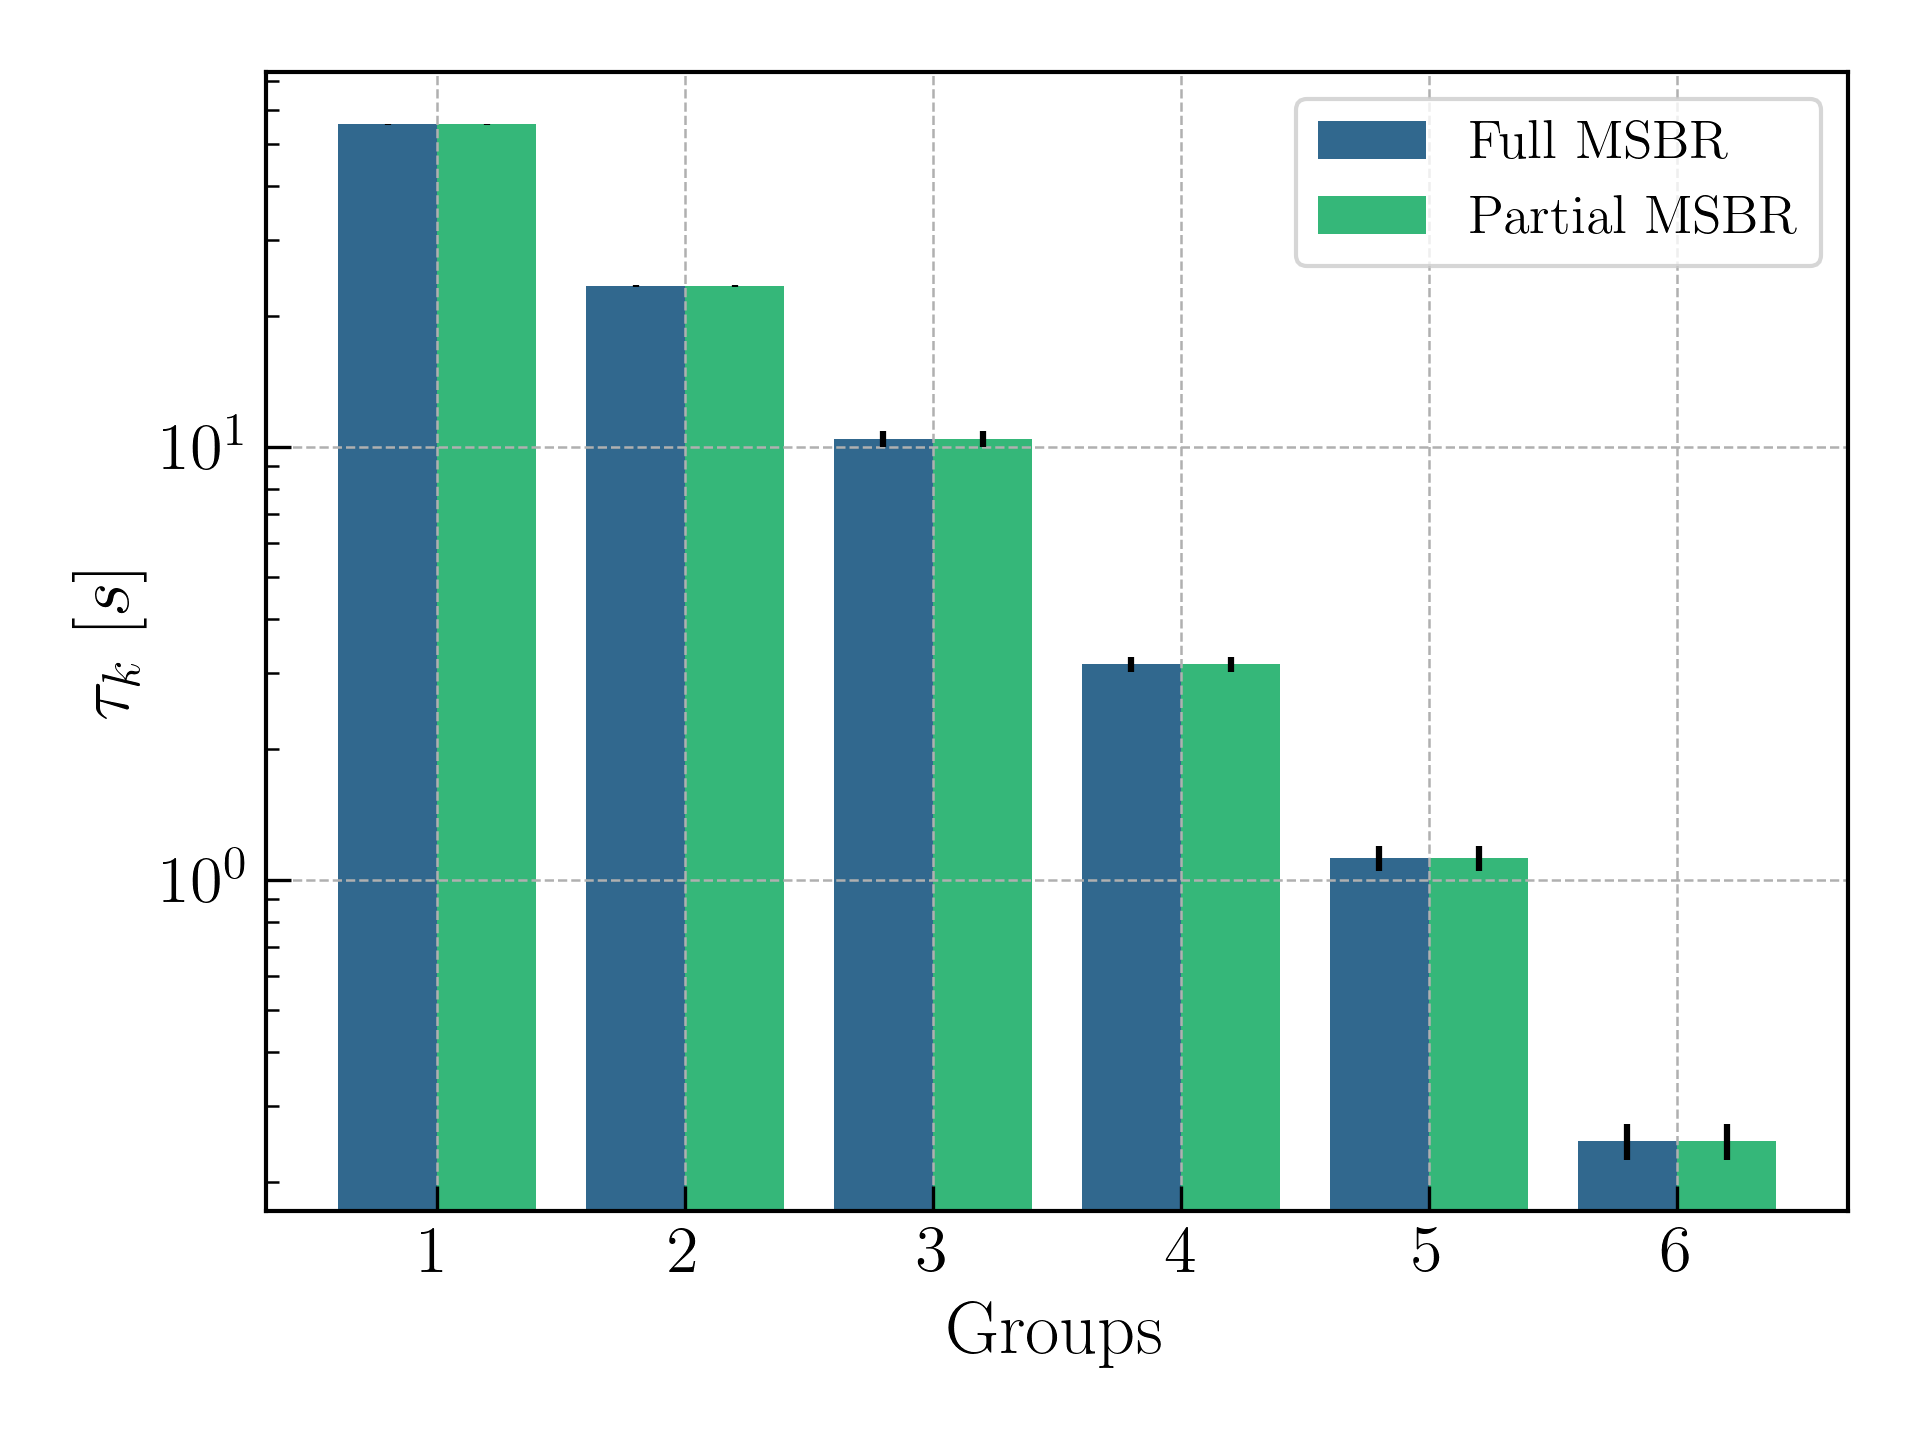
\includegraphics[width=1.0\linewidth]{../images/halflives_chem_long.png} 
            \caption{$\tau_k$ for each \gls{DNP} group $k$ after a thermal saturation irradiation of $^{235}$U using the 0D scaled model.}
        \end{figure} 
    \end{block}
    \column[t]{0.45\textwidth}
    \begin{block}{Group yields:}
        \begin{figure}[!ht]
            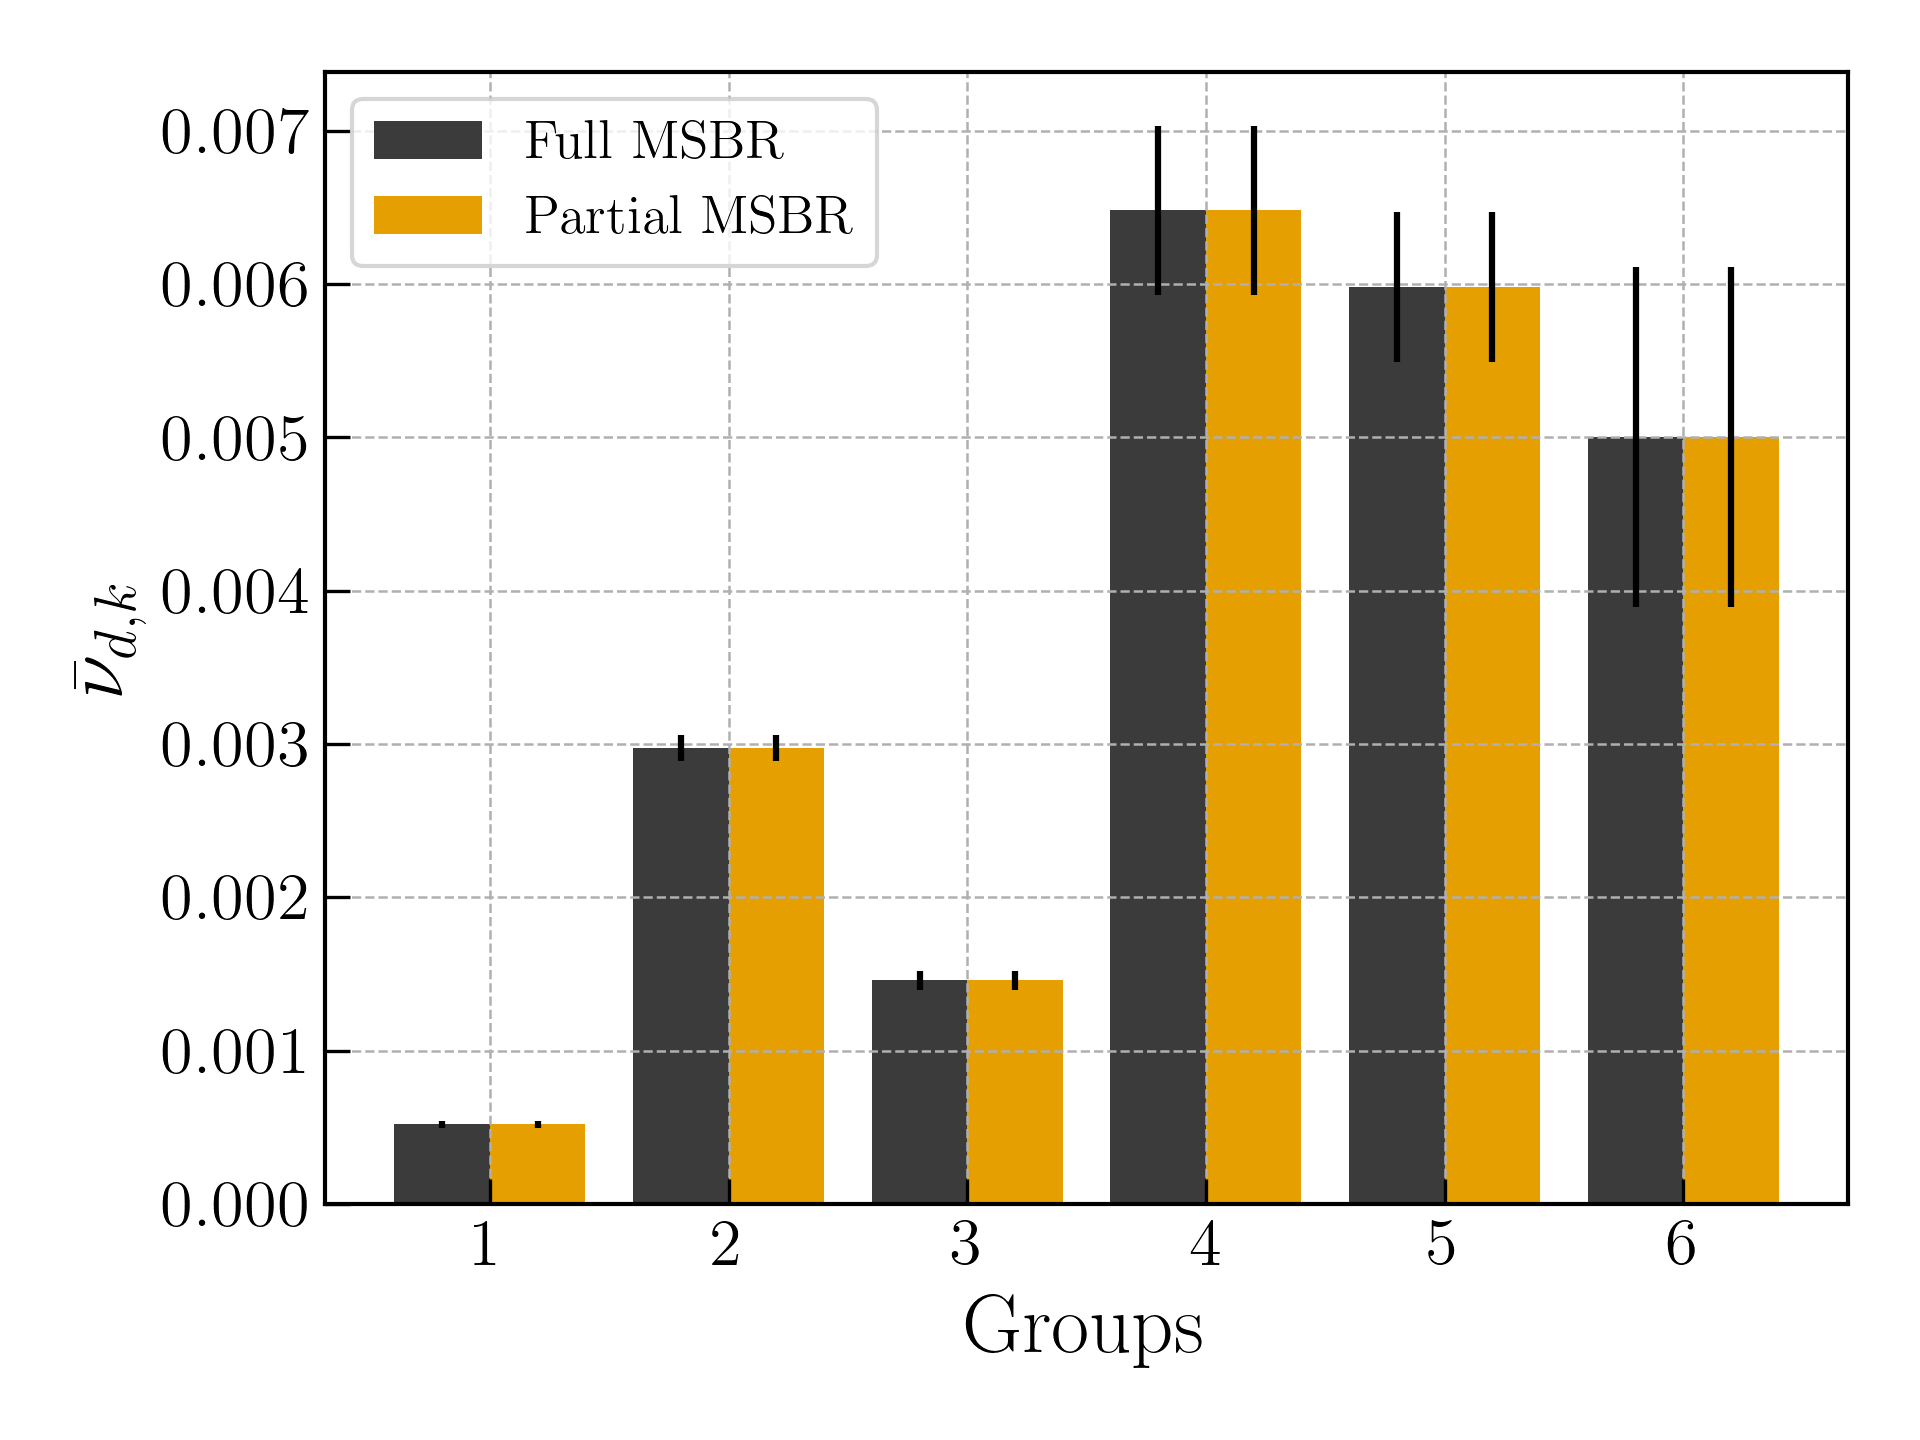
\includegraphics[width=1.0\linewidth]{../images/yields_chem_long.png} 
            \caption{$\bar{\nu}_{d,k}$ for each \gls{DNP} group $k$ after a thermal saturation irradiation of $^{235}$U using the 0D scaled model.}
        \end{figure} 
    \end{block}
\end{columns}
\textbf{The differences induced by exclusion of removal rates with cycle times longer than 20 seconds are minimal and well within uncertainty bounds.}
\end{frame}
\begin{frame}
\frametitle{Chemical removal rates have a small impact in the 0D scaled model}
\begin{columns}
    \column[t]{0.45\textwidth}
    \begin{block}{Group half-lives:}
        \begin{figure}[!ht]
            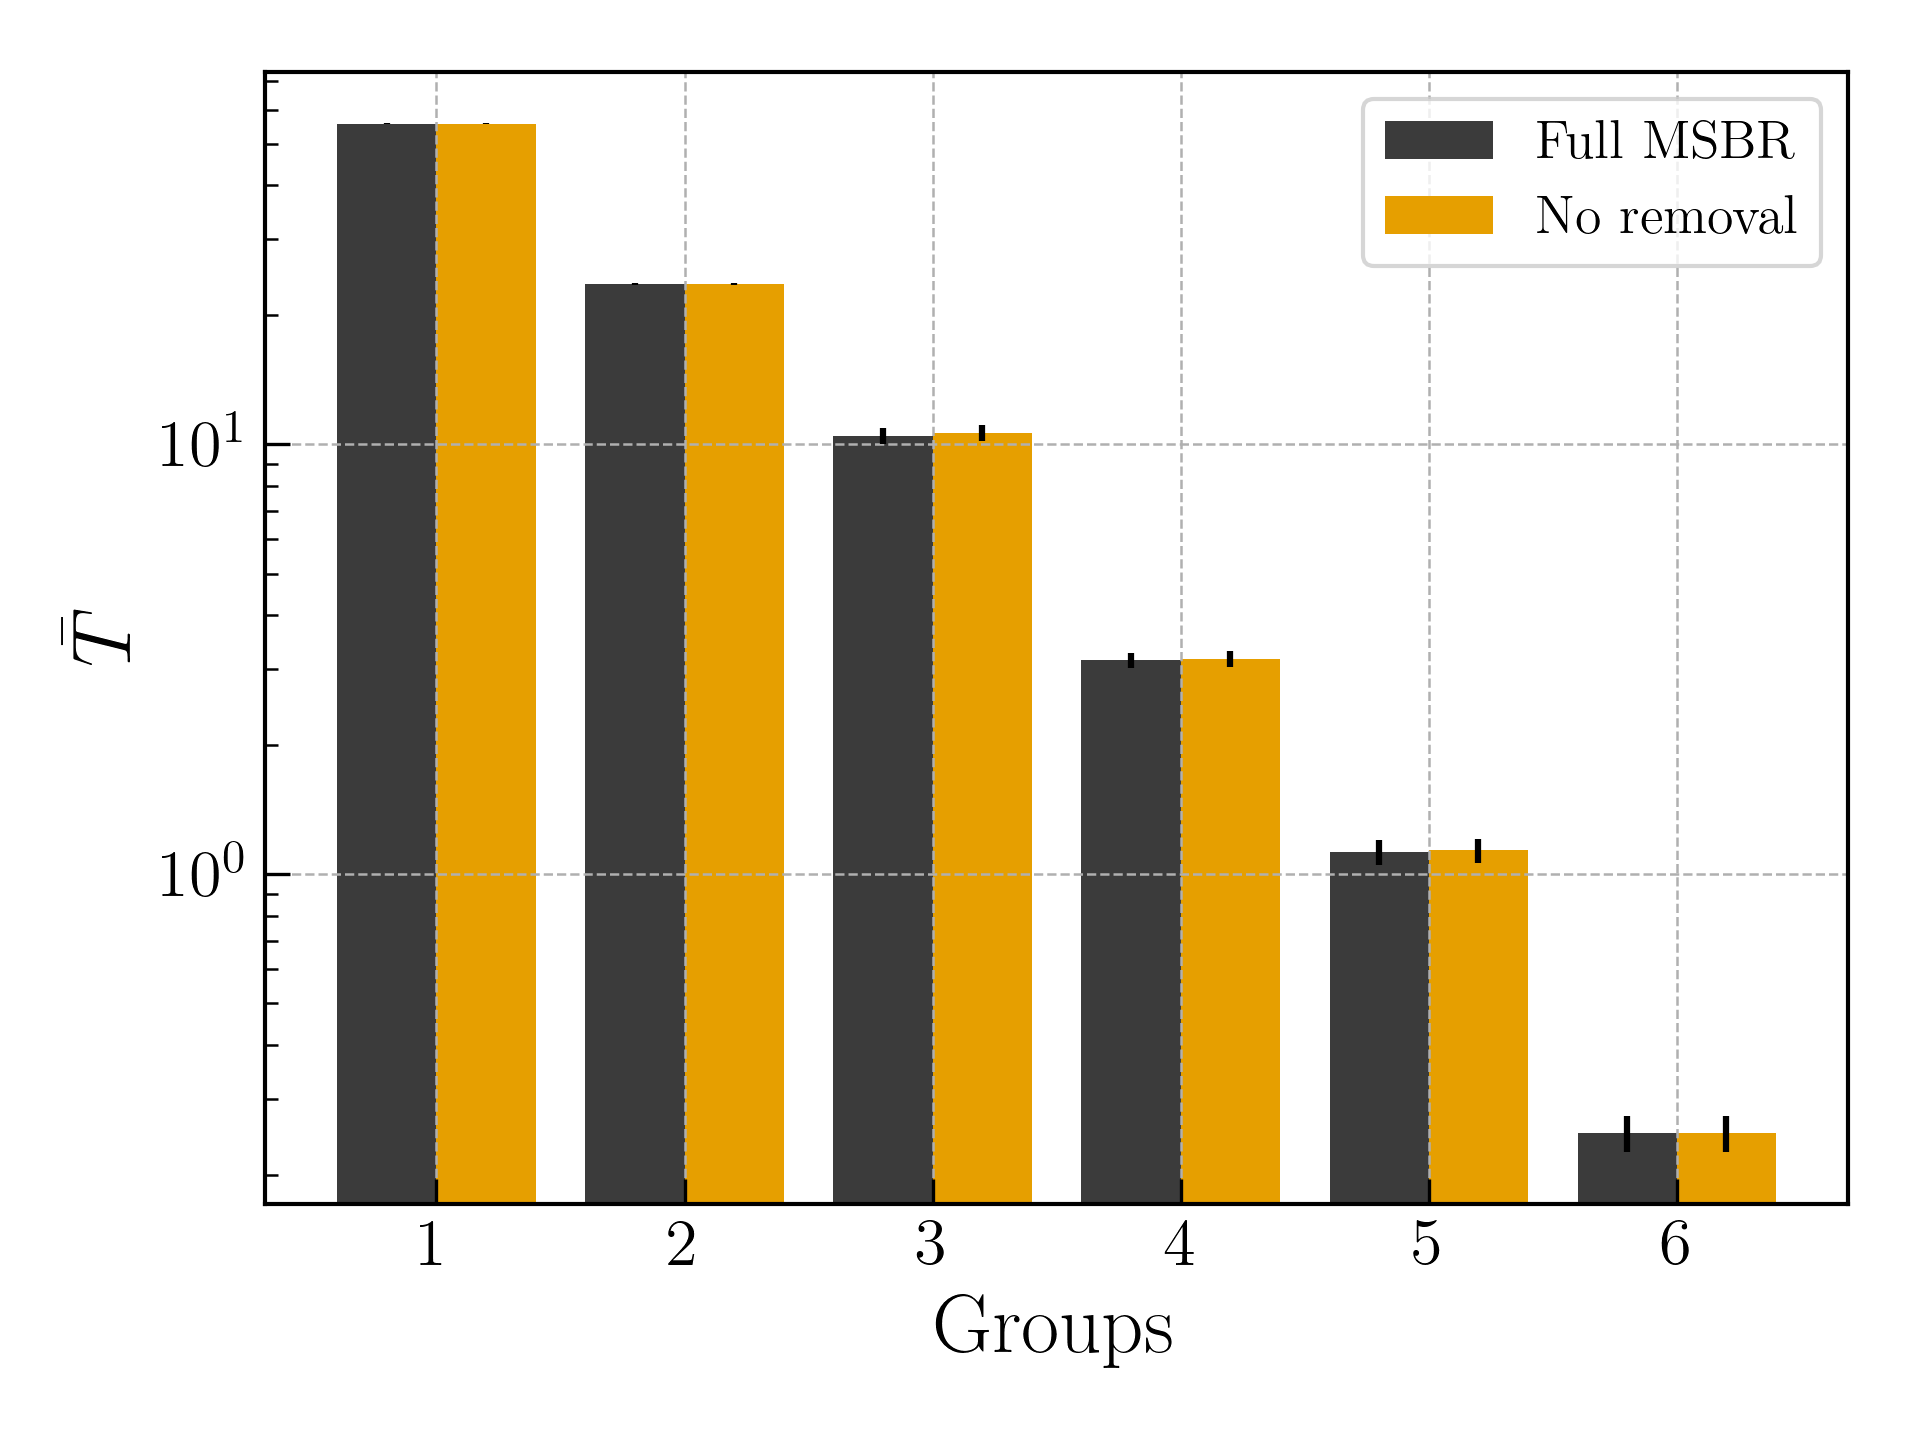
\includegraphics[width=1.0\linewidth]{../images/halflives_chem_bool.png} 
            \caption{$\tau_k$ for each \gls{DNP} group $k$ after a thermal saturation irradiation of $^{235}$U using the 0D scaled model.}
        \end{figure} 
    \end{block}
    \column[t]{0.45\textwidth}
    \begin{block}{Group yields:}
        \begin{figure}[!ht]
            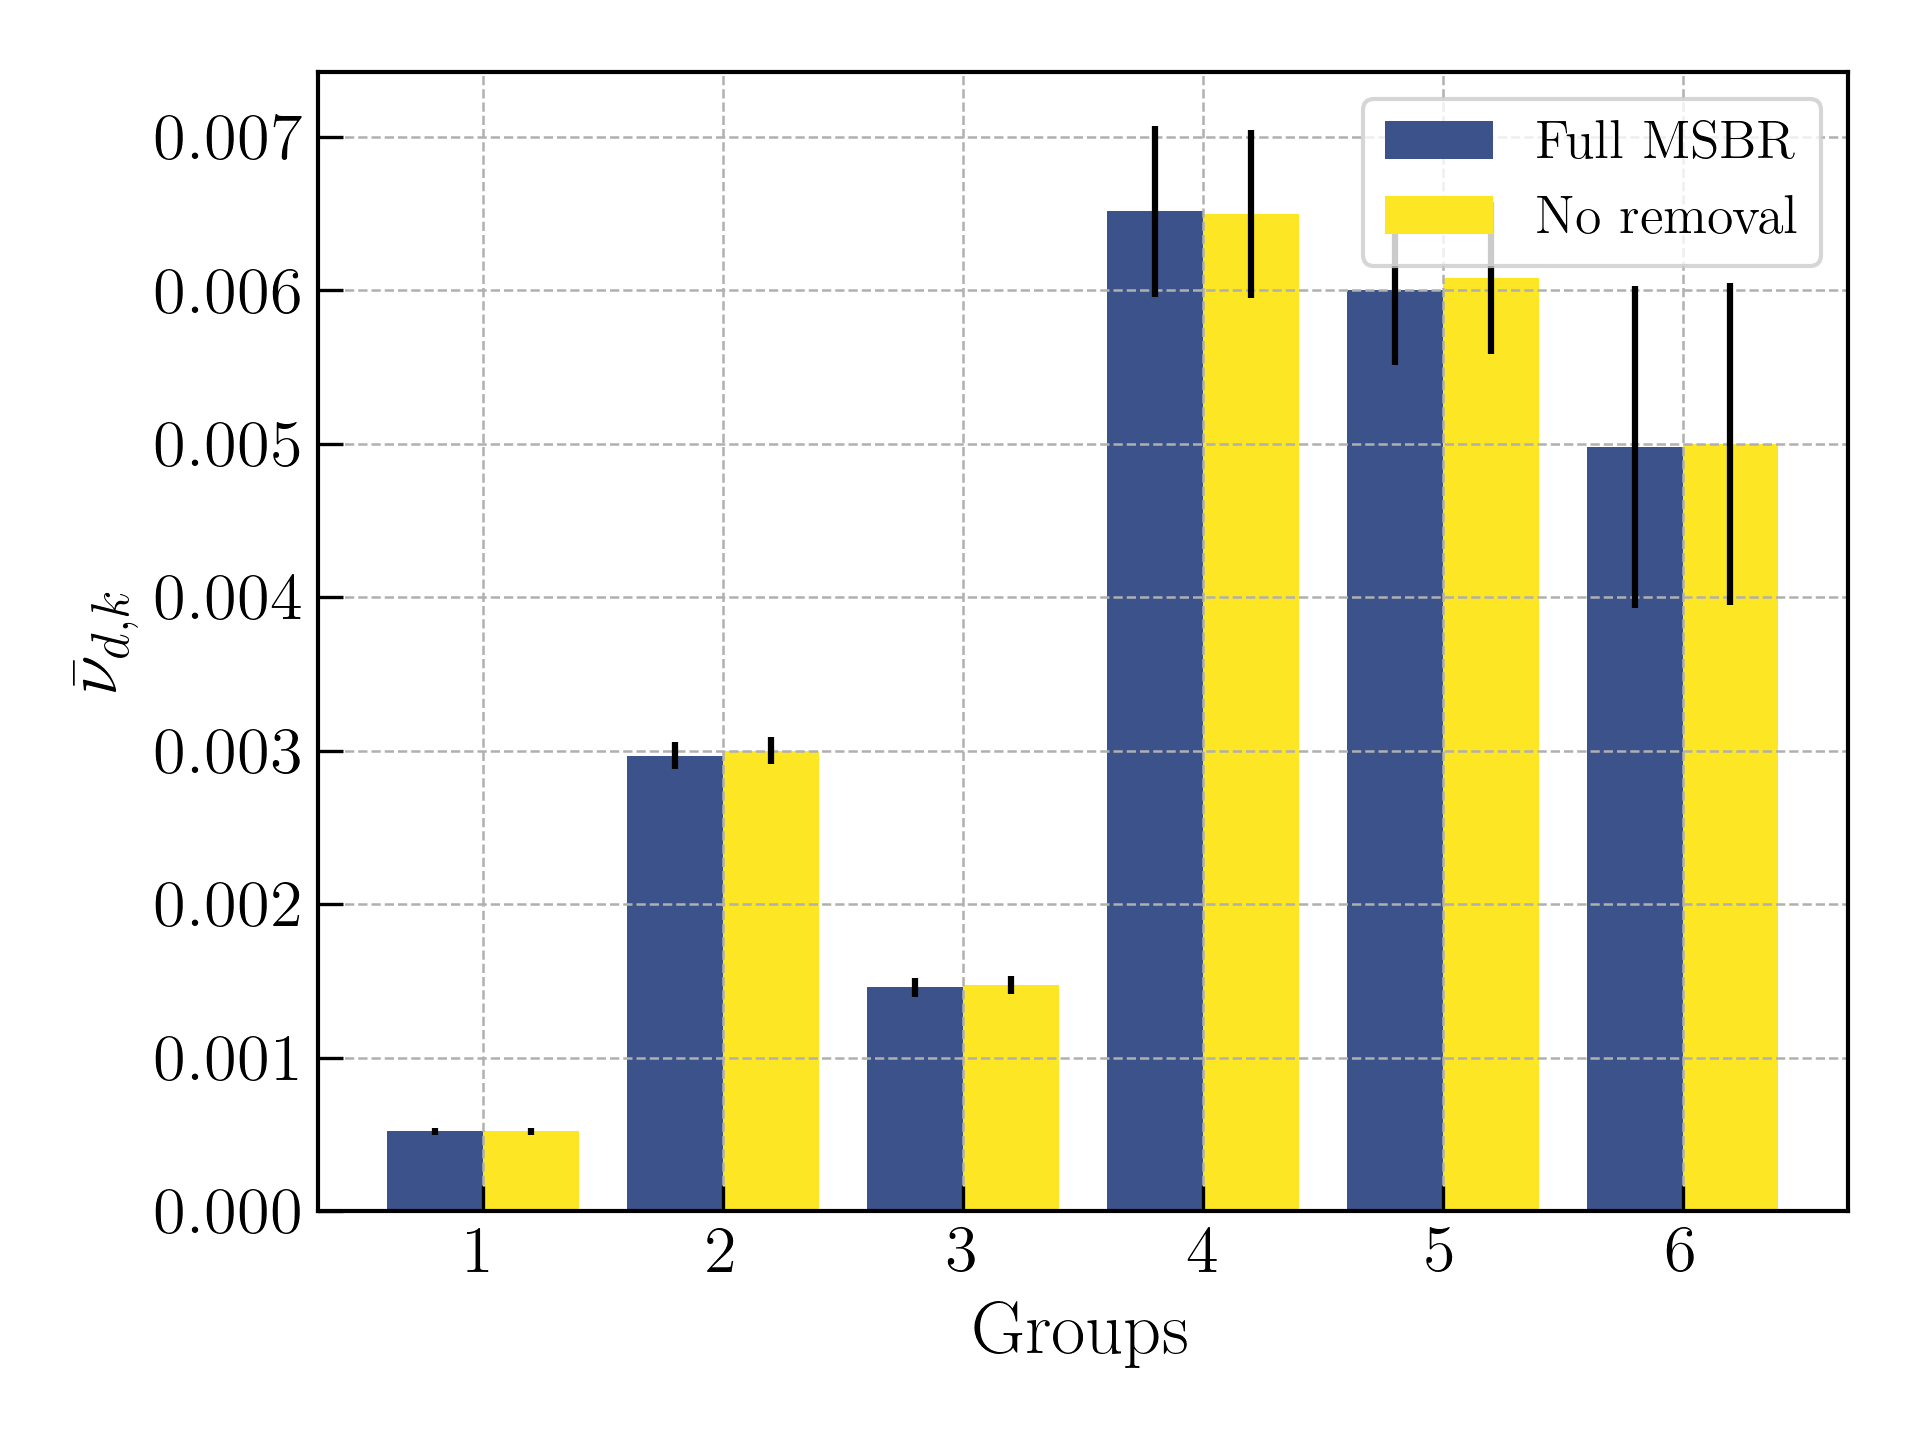
\includegraphics[width=1.0\linewidth]{../images/yields_chem_bool.png} 
            \caption{$\bar{\nu}_{d,k}$ for each \gls{DNP} group $k$ after a thermal saturation irradiation of $^{235}$U using the 0D scaled model.}
        \end{figure} 
    \end{block}
\end{columns}
\textbf{The differences induced by exclusion of removal rates with cycle times longer than 20 seconds are minimal and well within uncertainty bounds.Neglecting chemical removal rates generally leads to larger yields, though all differences are within uncertainty bounds.}

\end{frame}
\begin{frame}
\frametitle{Logarithmic spacing of time nodes give more accurate results}
\begin{columns}
    \column[t]{0.45\textwidth}
    \begin{block}{Group half-lives:}
        \begin{figure}[!ht]
            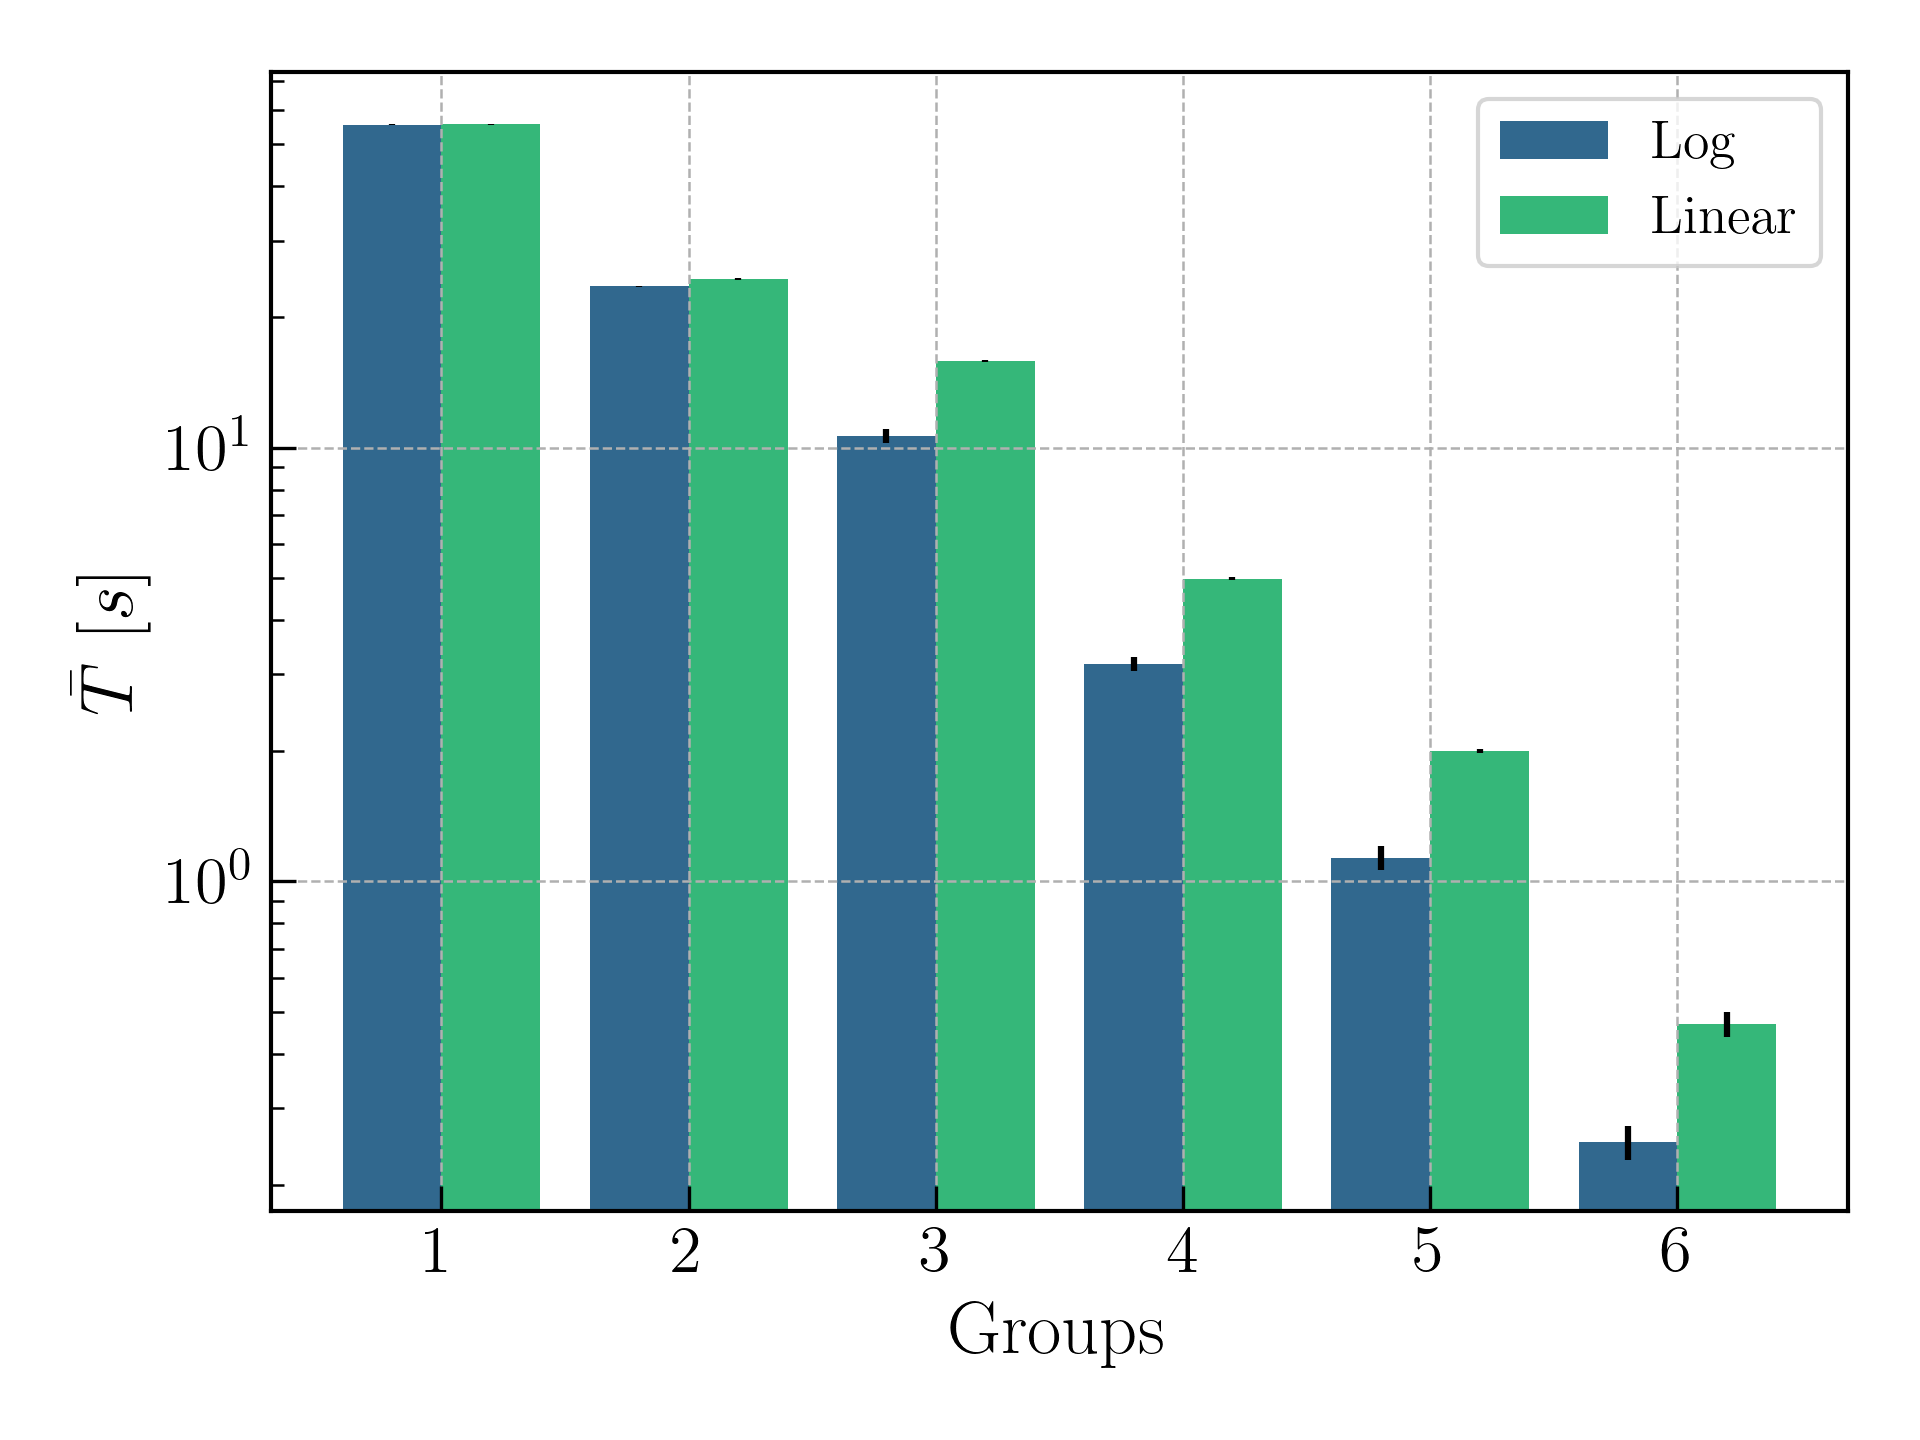
\includegraphics[width=1.0\linewidth]{../images/halflives_spacing_times.png} 
            \caption{$\tau_k$ for each \gls{DNP} group $k$ after a thermal saturation irradiation of $^{235}$U using the 0D scaled model.}
        \end{figure} 
    \end{block}
    \column[t]{0.45\textwidth}
    \begin{block}{Group yields:}
        \begin{figure}[!ht]
            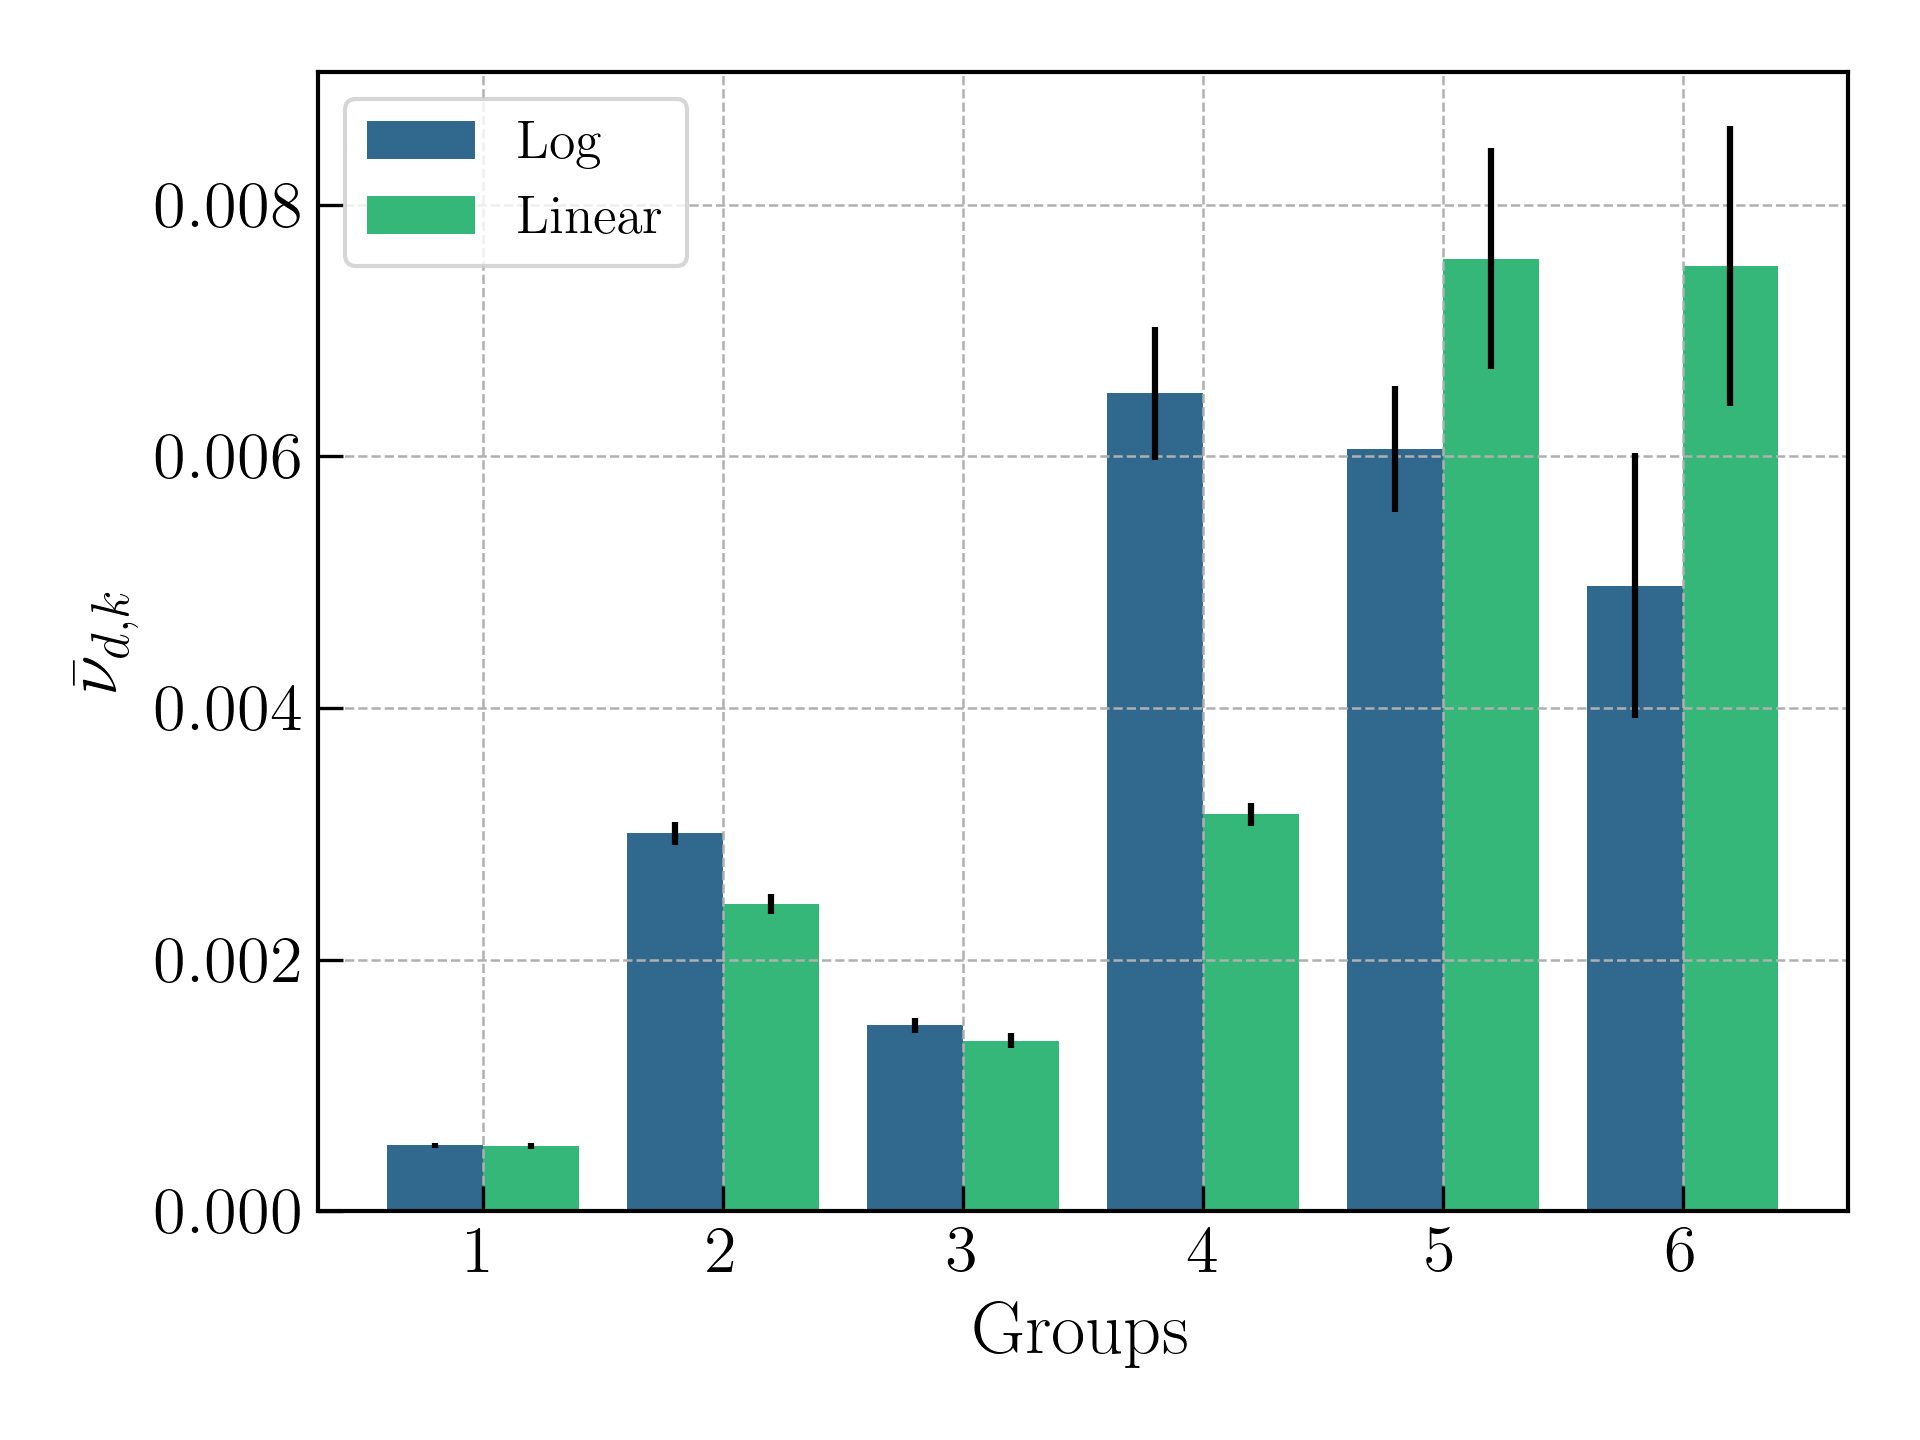
\includegraphics[width=1.0\linewidth]{../images/yields_spacing_times.png} 
            \caption{$\bar{\nu}_{d,k}$ for each \gls{DNP} group $k$ after a thermal saturation irradiation of $^{235}$U using the 0D scaled model.}
        \end{figure} 
    \end{block}
\end{columns}
\textbf{Linear spacing has no data between zero and two seconds, and it places greater weight on longer-lived groups due to the data distribution.}
\end{frame}
\begin{frame}
\frametitle{Logarithmic spacing of time nodes give more accurate results}
\begin{columns}
    \column[t]{0.45\textwidth}
    \begin{block}{Group half-lives:}
        \begin{figure}[!ht]
            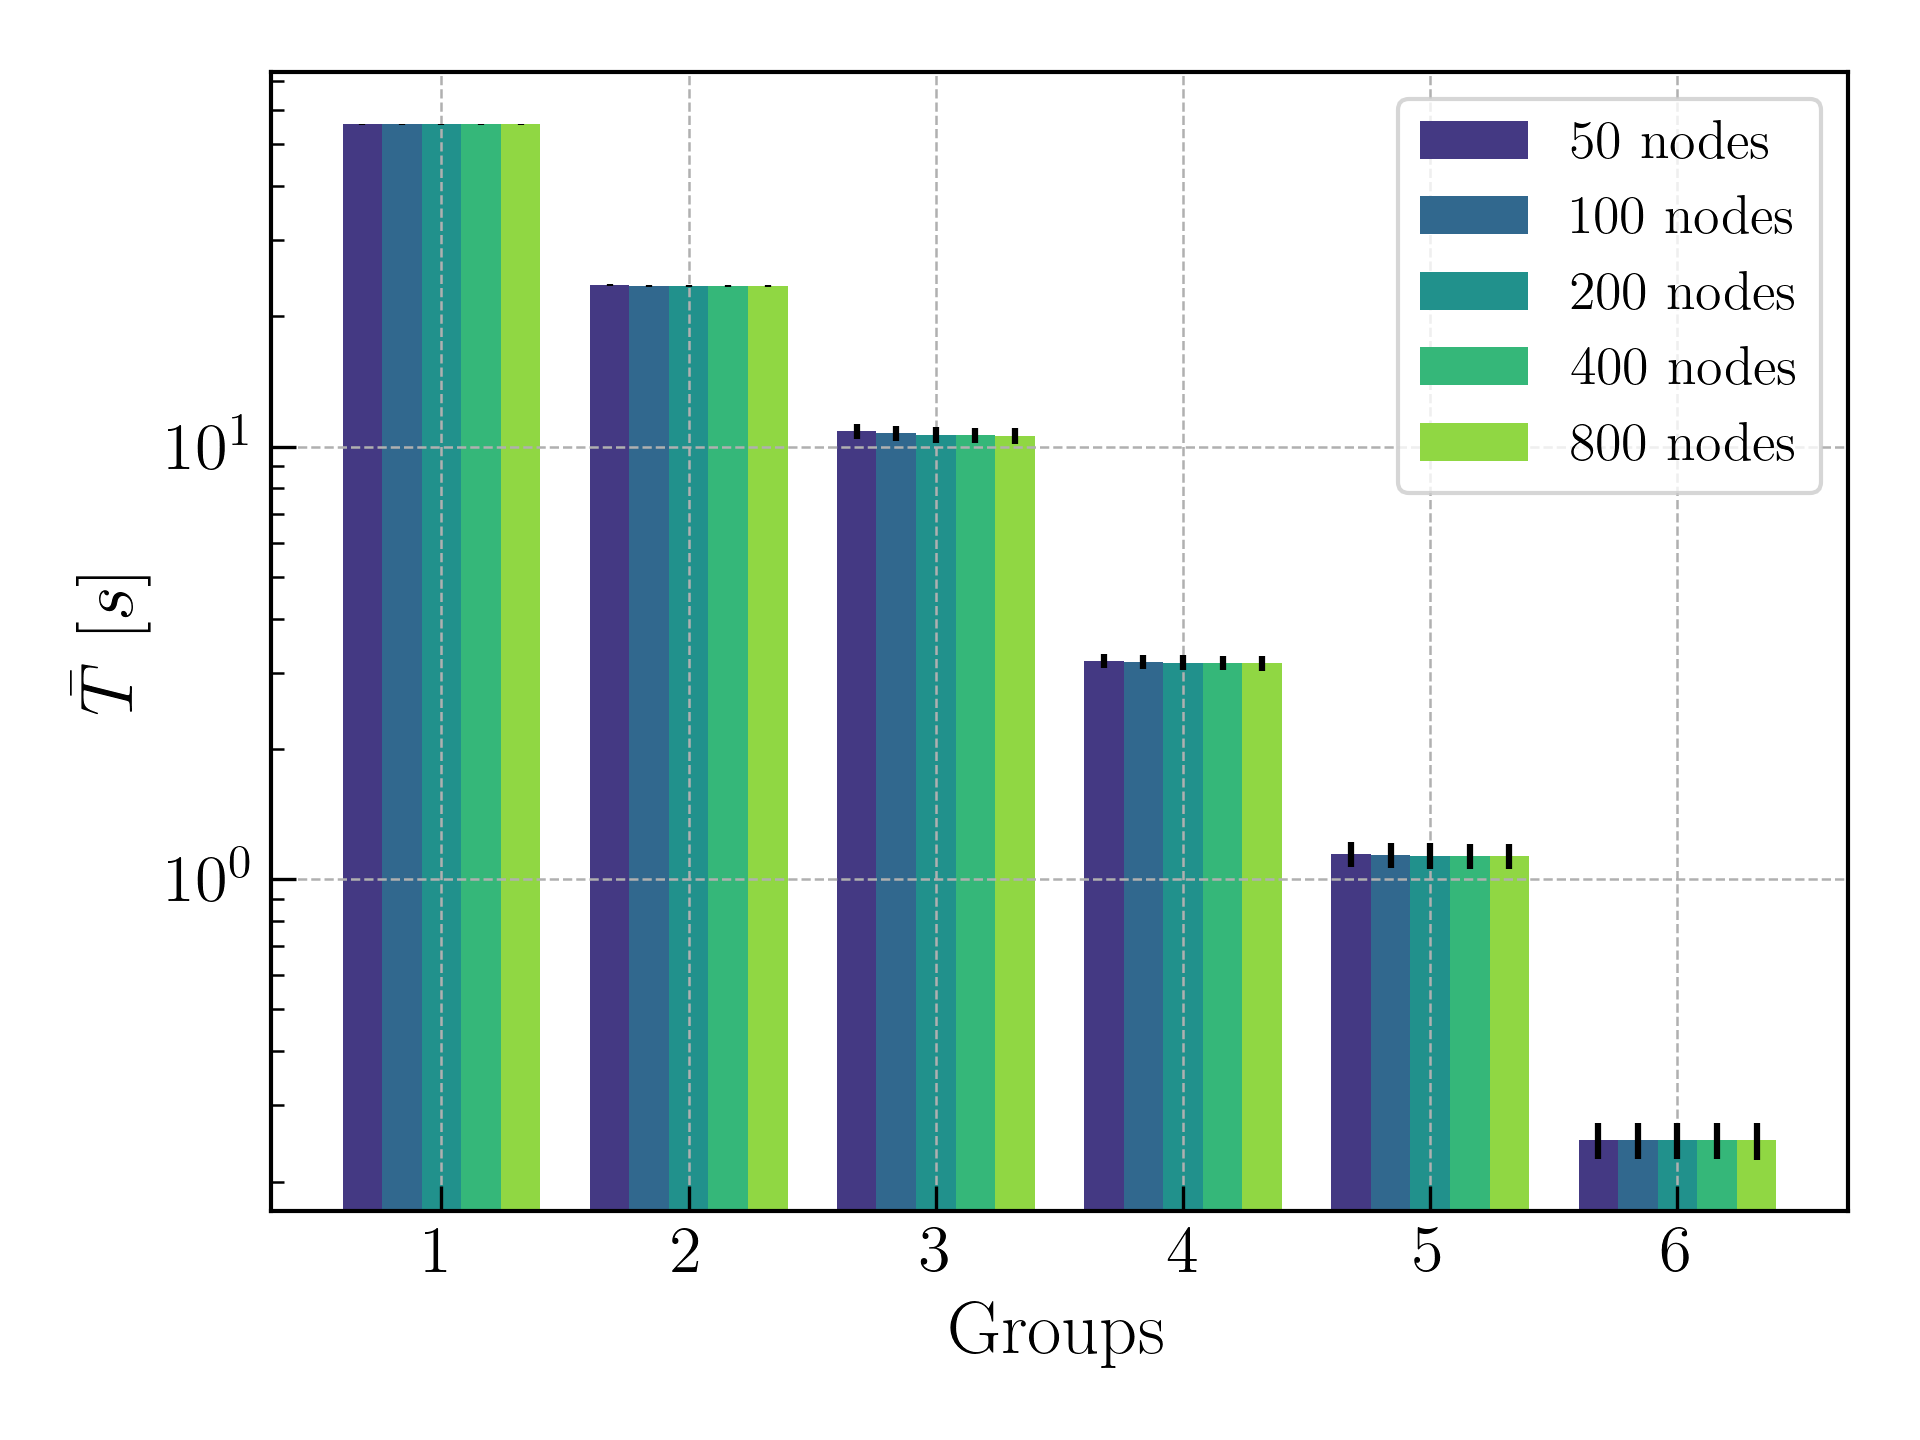
\includegraphics[width=1.0\linewidth]{../images/halflives_decay_time_nodes.png} 
            \caption{$\tau_k$ for each \gls{DNP} group $k$ after a thermal saturation irradiation of $^{235}$U using the 0D scaled model.}
        \end{figure} 
    \end{block}
    \column[t]{0.45\textwidth}
    \begin{block}{Group yields:}
        \begin{figure}[!ht]
            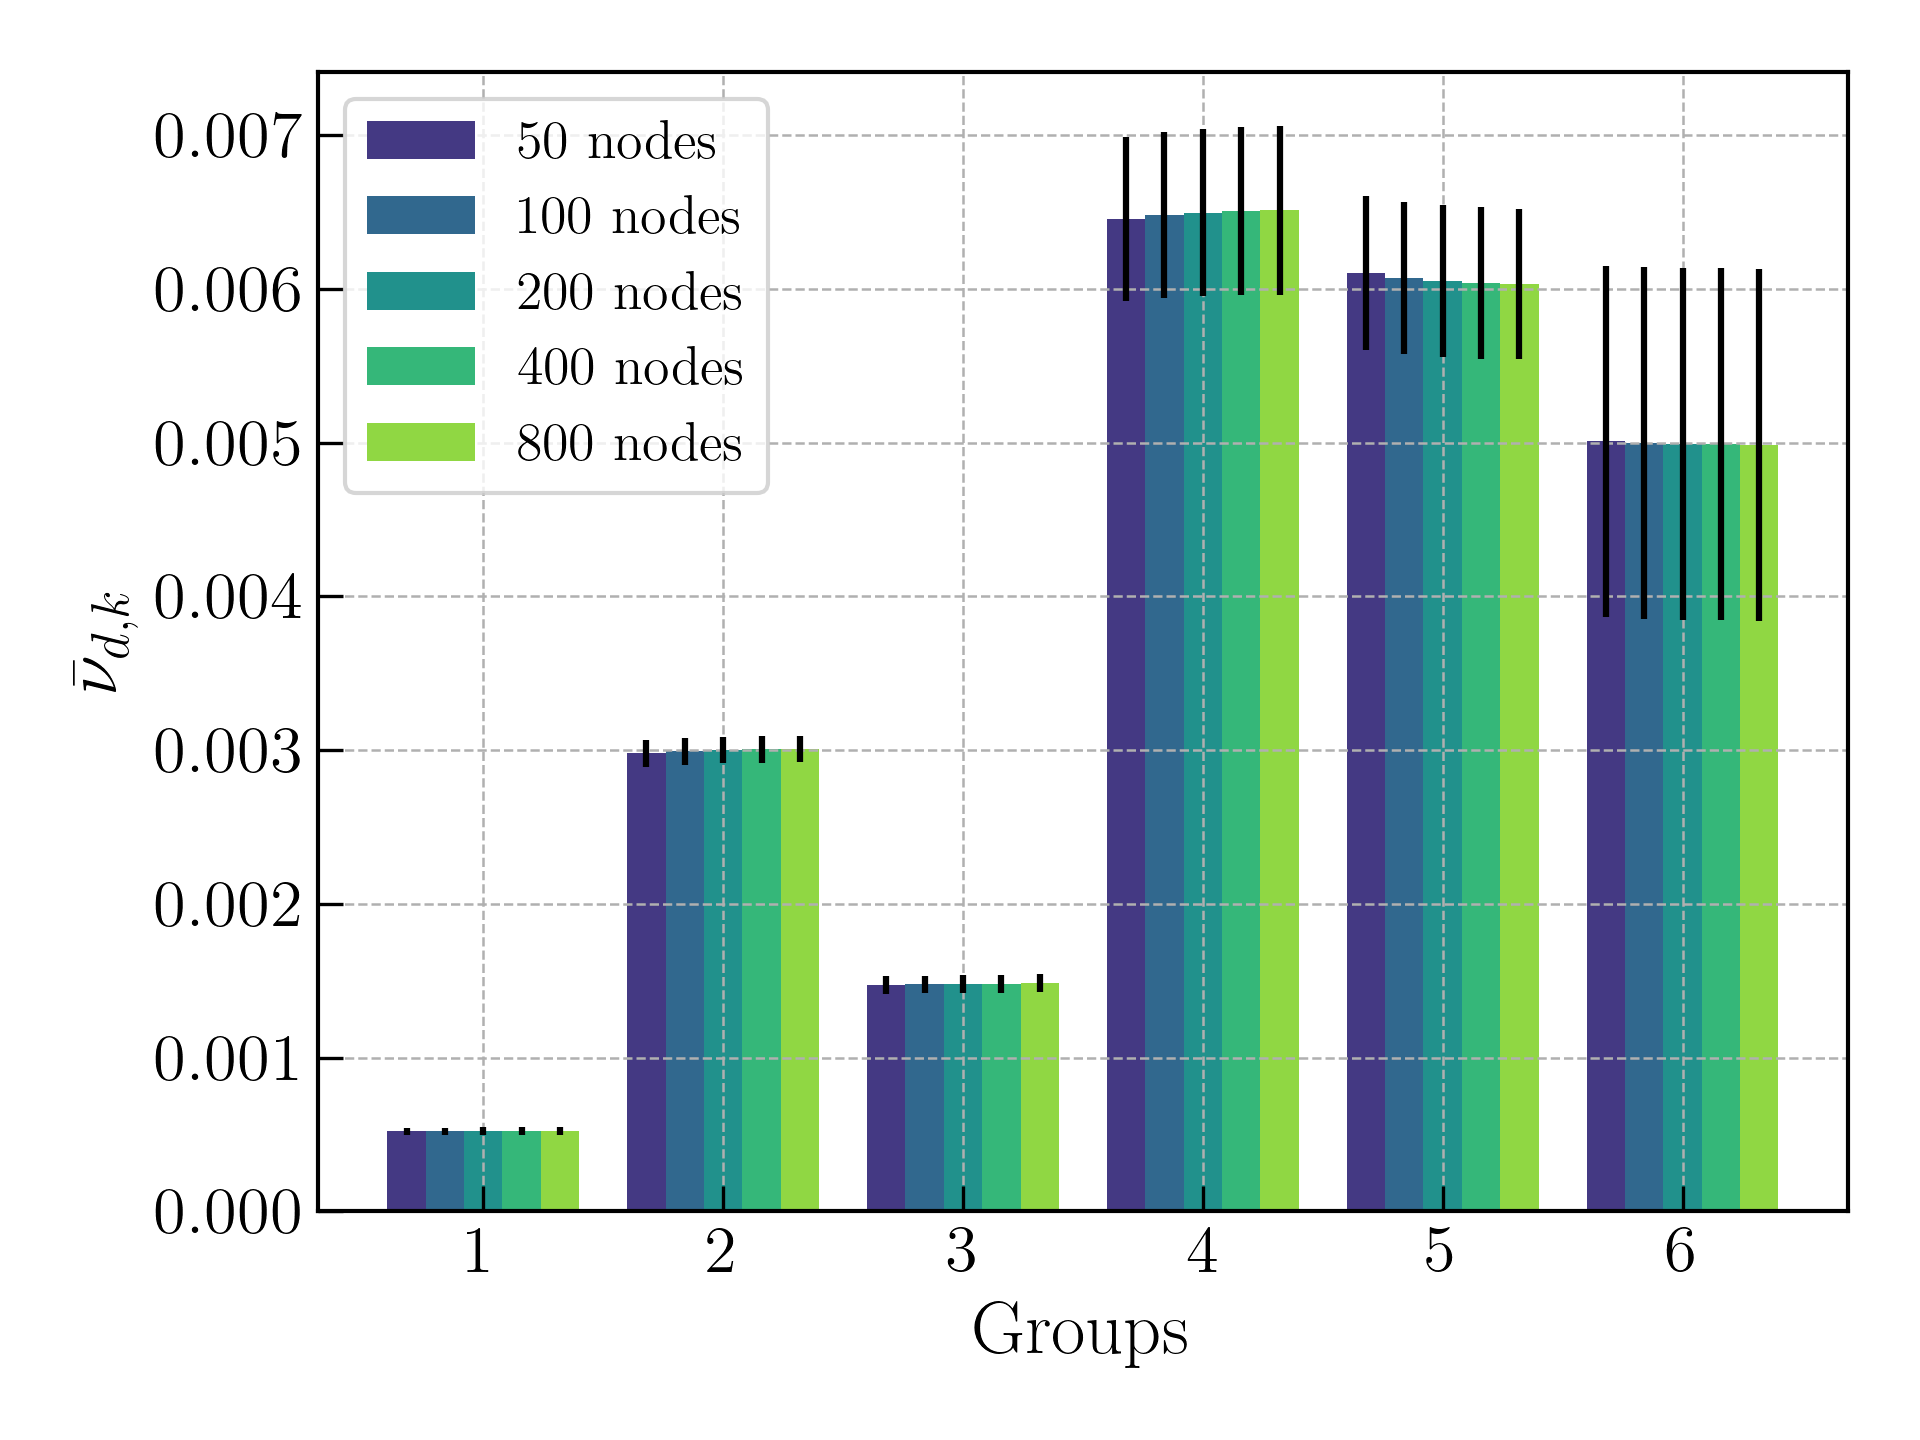
\includegraphics[width=1.0\linewidth]{../images/yields_decay_time_nodes.png} 
            \caption{$\bar{\nu}_{d,k}$ for each \gls{DNP} group $k$ after a thermal saturation irradiation of $^{235}$U using the 0D scaled model.}
        \end{figure} 
    \end{block}
\end{columns}
\textbf{Increasing the number of nodes increases the accuracy of the \gls{DNP} group parameters, with differences in the yields that are within uncertainty bounds.}
\end{frame}
\begin{frame}
\frametitle{Longer measurement times give more accurate results}
\begin{columns}
    \column[t]{0.45\textwidth}
    \begin{block}{Group half-lives:}
        \begin{figure}[!ht]
            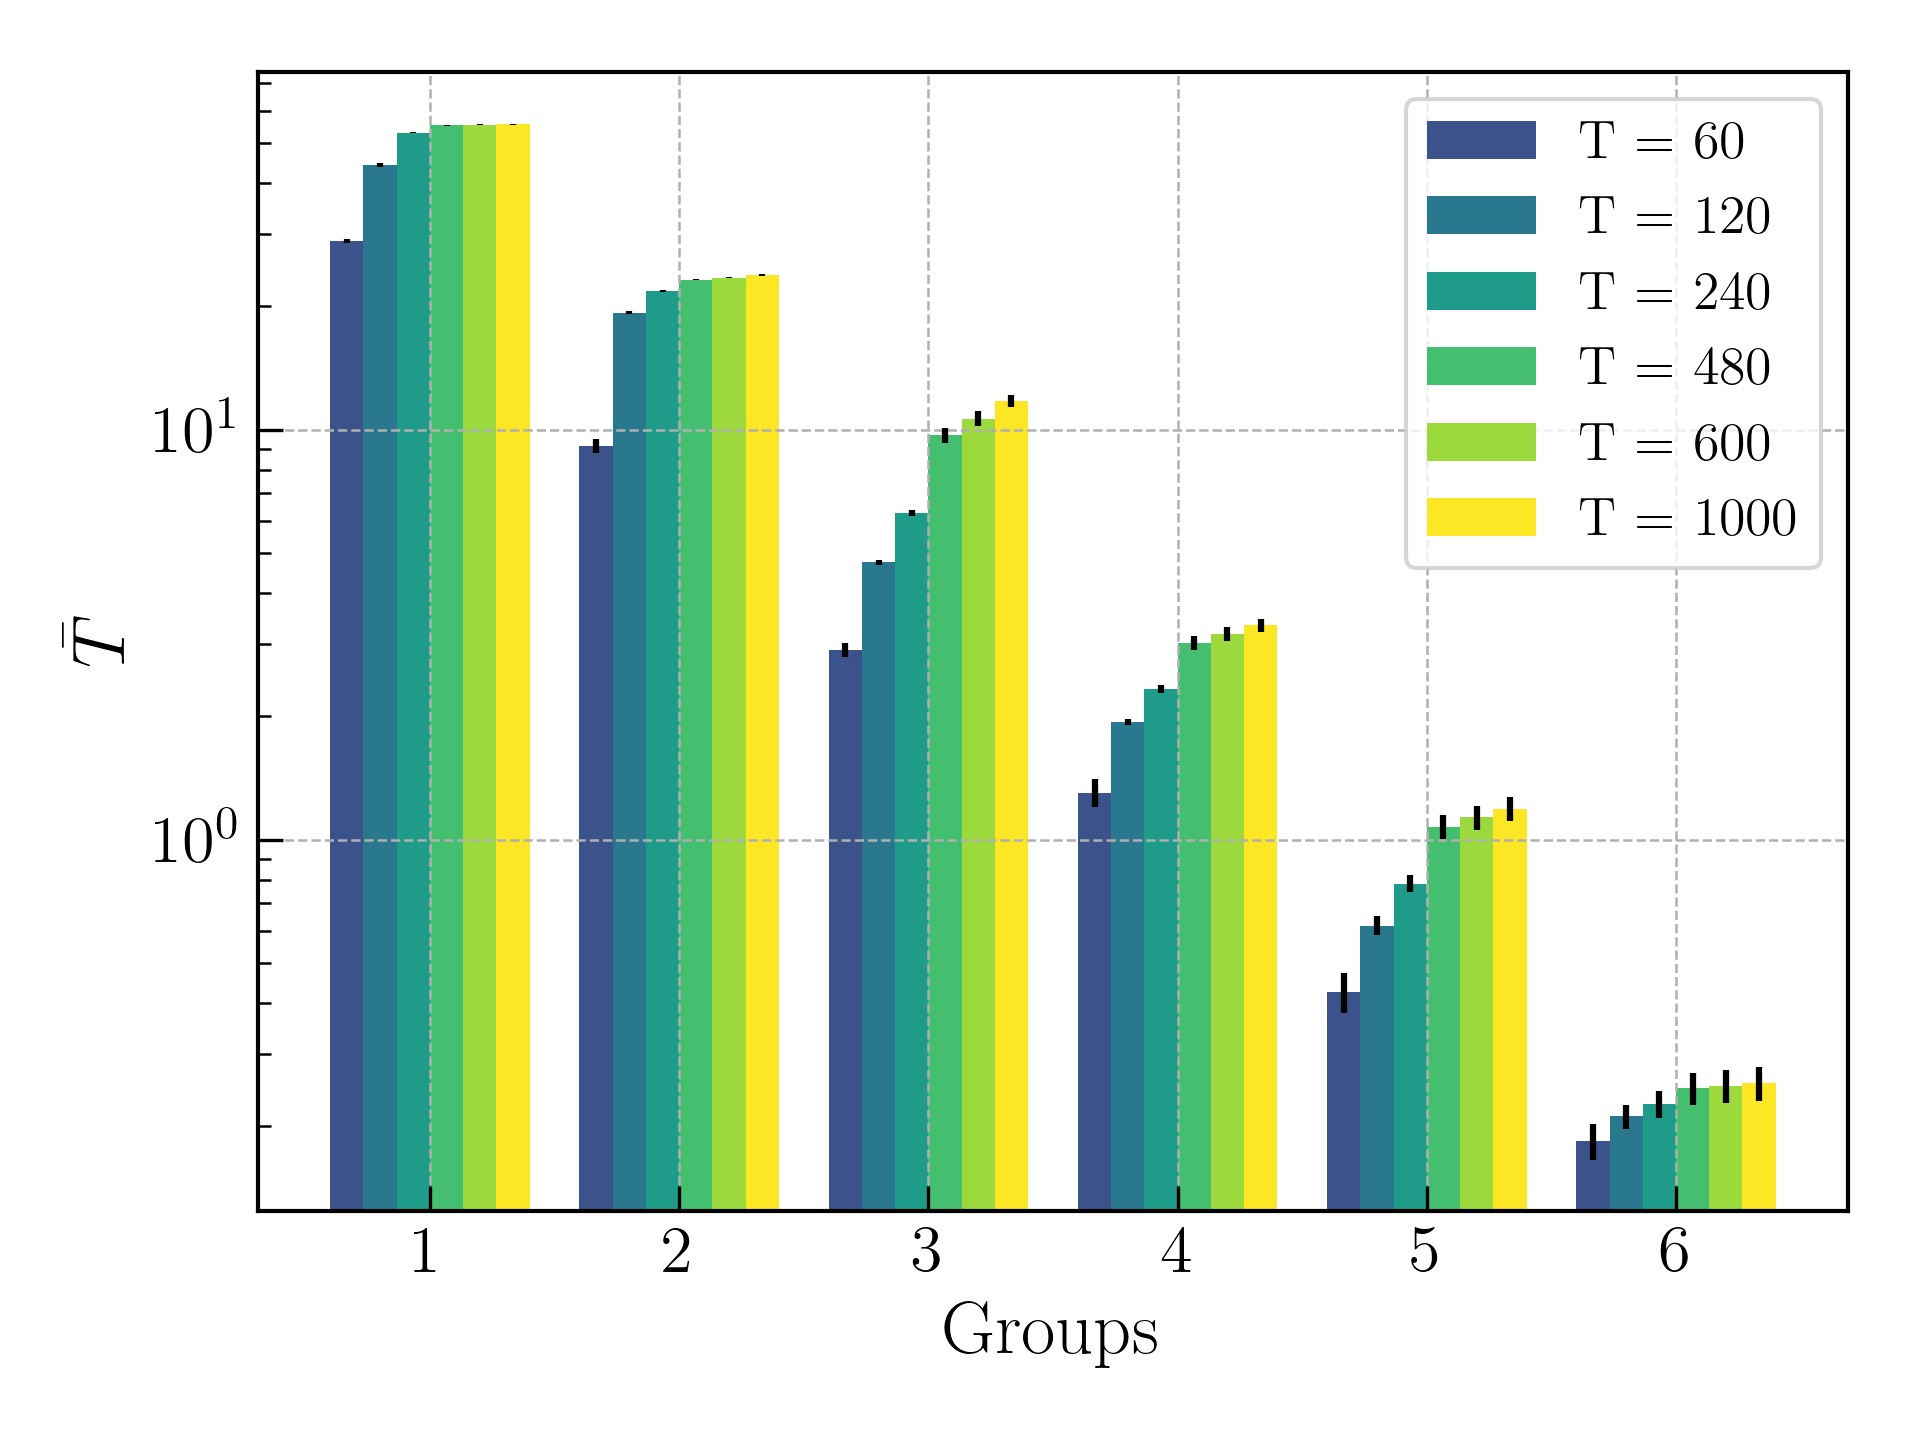
\includegraphics[width=1.0\linewidth]{../images/halflives_total_decay_time.png} 
            \caption{$\tau_k$ for each \gls{DNP} group $k$ after a thermal saturation irradiation of $^{235}$U using the 0D scaled model.}
        \end{figure} 
    \end{block}
    \column[t]{0.45\textwidth}
    \begin{block}{Group yields:}
        \begin{figure}[!ht]
            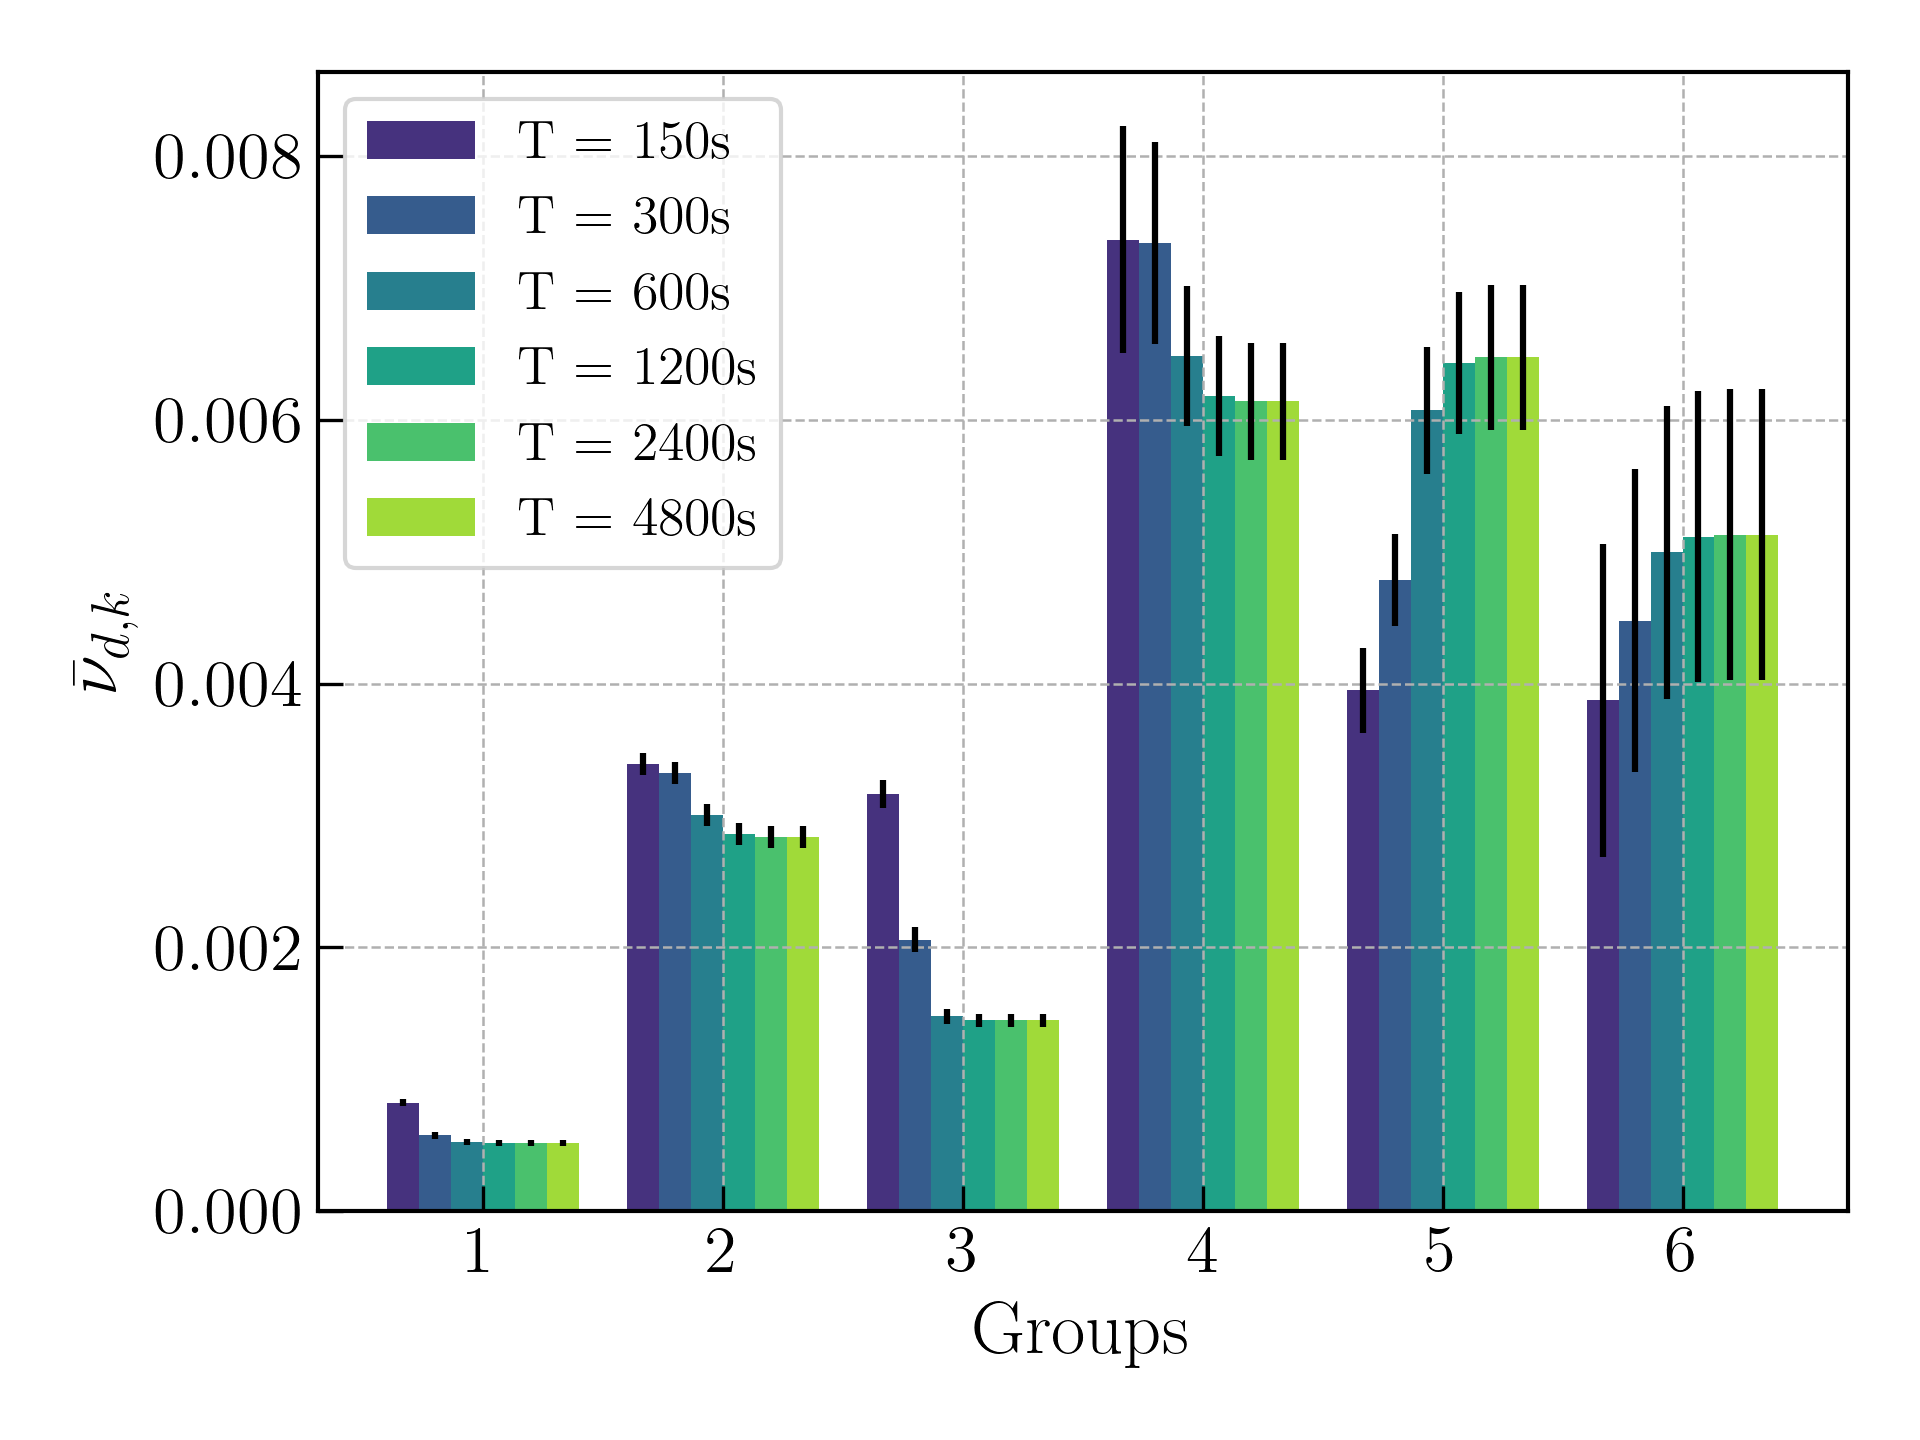
\includegraphics[width=1.0\linewidth]{../images/yields_total_decay_time.png} 
            \caption{$\bar{\nu}_{d,k}$ for each \gls{DNP} group $k$ after a thermal saturation irradiation of $^{235}$U using the 0D scaled model.}
        \end{figure} 
    \end{block}
\end{columns}
\textbf{Longer post-irradiation time results in longer-lived groups with smaller yields in groups one through four and larger yields in groups five and six.}
\end{frame}
\begin{frame}
\frametitle{The density of time nodes does not drive the group parameters}
\begin{columns}
    \column[t]{0.45\textwidth}
    \begin{block}{Group half-lives:}
        \begin{figure}[!ht]
            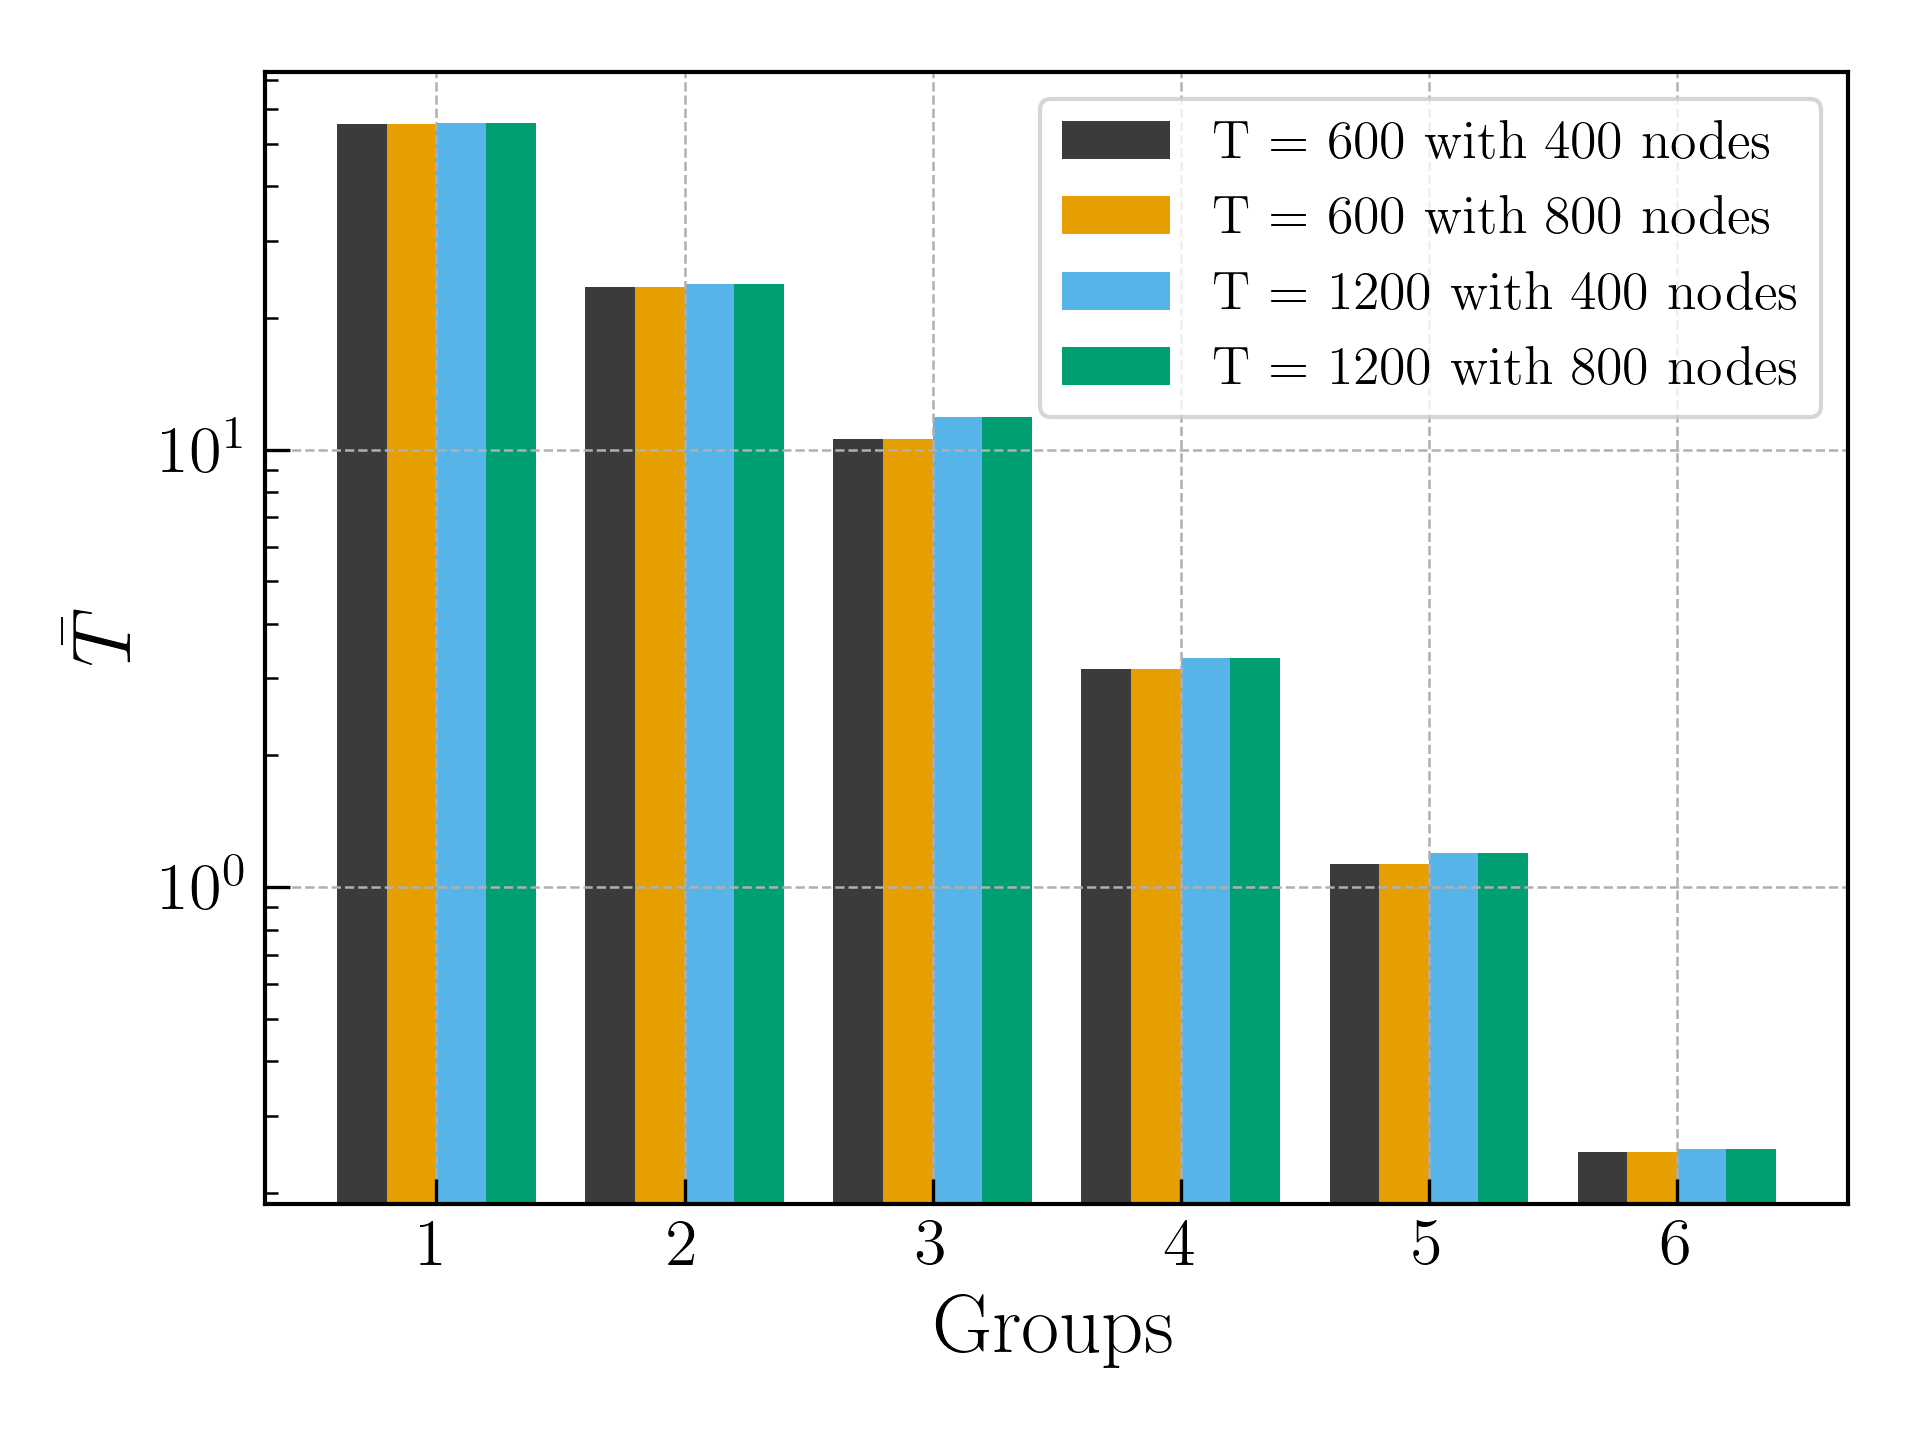
\includegraphics[width=1.0\linewidth]{../images/halflives_detailed_decay.png} 
            \caption{$\tau_k$ for each \gls{DNP} group $k$ after a thermal saturation irradiation of $^{235}$U using the 0D scaled model.}
        \end{figure} 
    \end{block}
    \column[t]{0.45\textwidth}
    \begin{block}{Group yields:}
        \begin{figure}[!ht]
            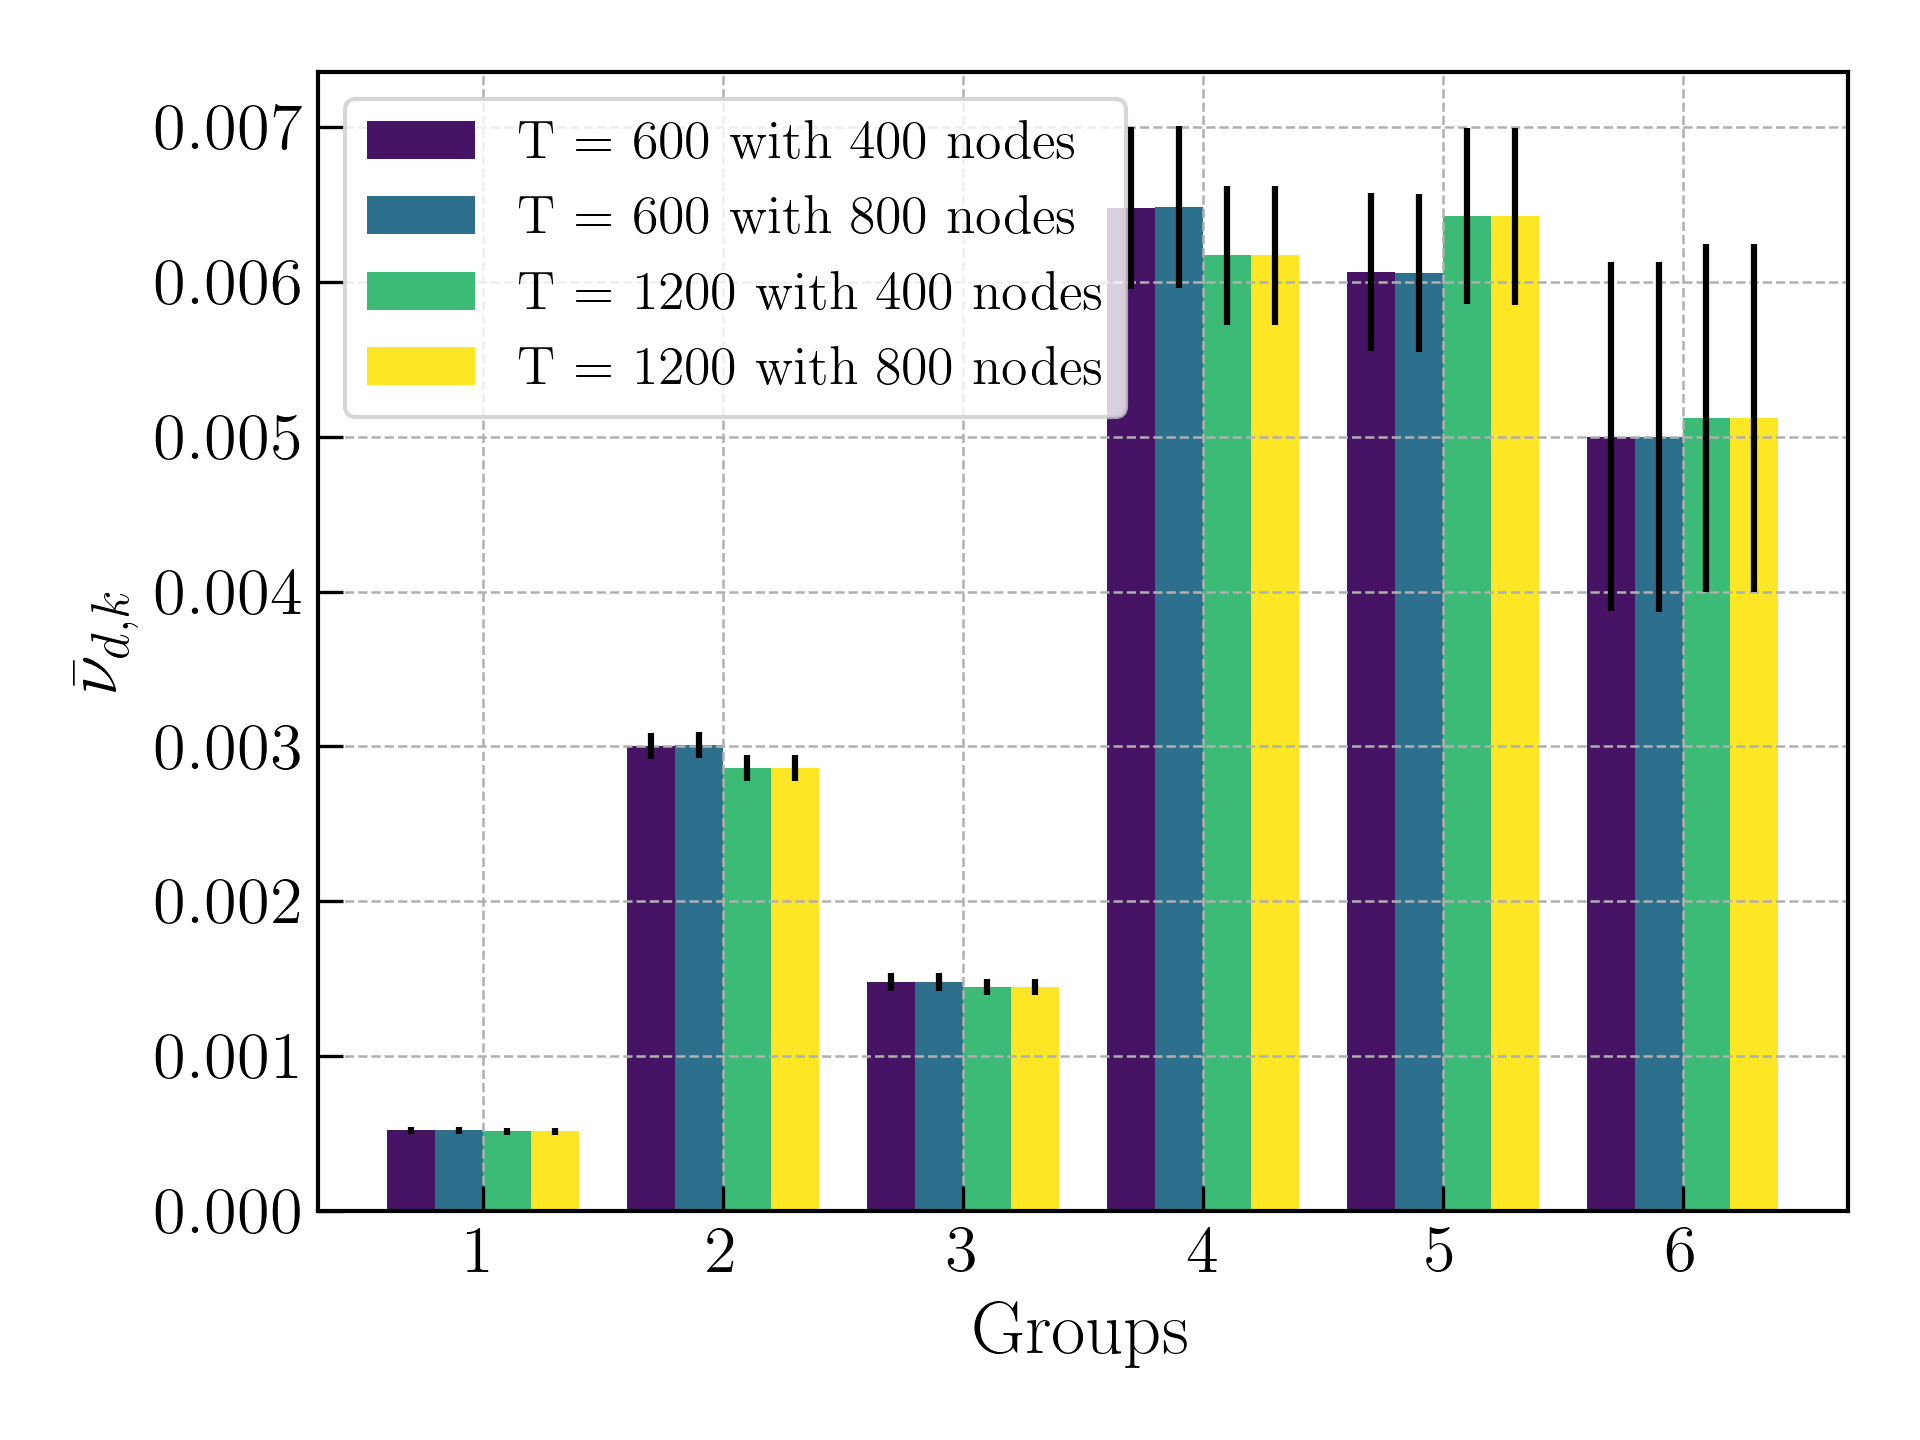
\includegraphics[width=1.0\linewidth]{../images/yields_detailed_decay.png} 
            \caption{$\bar{\nu}_{d,k}$ for each \gls{DNP} group $k$ after a thermal saturation irradiation of $^{235}$U using the 0D scaled model.}
        \end{figure} 
    \end{block}
\end{columns}
\textbf{The number of nodes has a small impact on the \gls{DNP} group parameters, whereas the total decay time causes larger differences.}
\end{frame}
\begin{frame}
  \frametitle{Safety-related transients may disrupt safe reactor operation}
    \begin{block}{Safety-related transients that will be modeled are:}
        \begin{itemize}
            \item \Gls{ULOHS}
            \begin{itemize}
                \item Loss of cooling in the reactor, potentially due to a heat exchanger failure
                \item Modeled in Moltres by setting inlet temperature equal to outlet temperature
            \end{itemize}
            \item \Gls{ULOF}
            \begin{itemize}
                \item Flow rate decreases to zero due to a pump failure
                \item Modeled in Moltres by changing flow field over time to match \gls{MSRE} pump shut-down
            \end{itemize}
            \item \Gls{UTOP}
            \begin{itemize}
                \item Reactivity insertion event, which could be caused by poison removal, fissile addition, or temperature change
                \item Modeled in Moltres by having a step-decrease in the removal cross section, representing control rod withdrawal
            \end{itemize}
            \item \Gls{FSOC}
            \begin{itemize}
                \item Fuel salt temperature decreases, potentially caused by increased heat removal rate
                \item Modeled in Moltres by reducing inlet temperature by 25\%
            \end{itemize}
        \end{itemize}
    \end{block}
\end{frame}



\begin{frame}
  \frametitle{Sabotage may be used as a diversion}
  This framework assumes a hostile actor and an insider with the objective to disrupt operations \cite{protection2011evaluation}.
    \begin{block}{Sabotage-initiated transients that will be modeled are:}
        \begin{itemize}
            \item All safety-related transients as single events
            \item Combined \Gls{UTOP} and \gls{ULOHS}
            \begin{itemize}
                \item This should cause a temperature increase that propagates due to lack of heat sink; reactivity should then decrease due to temperature increase
            \end{itemize}
            \item Combined \Gls{UTOP} and \gls{ULOF}
            \begin{itemize}
                \item This should cause a temperature increase with a peak maximum temperature due to the stationary fuel salt; reactivity should then decrease due to temperature increase
            \end{itemize}
            \item Combined \Gls{UTOP} and \gls{FSOC}
            \begin{itemize}
                \item This should cause a temperature increase that is counteracted by the overcooled inlet fuel salt, leading to the largest reactivity change; temperature is not expected to change dramatically
            \end{itemize}
        \end{itemize}
    \end{block}
\end{frame}




\end{document}
